\chapter{Double Higgs Boson Production Analysis}
\label{chap:DoubleHiggs}

\chapterquote{The supreme art of war is to subdue the enemy without fighting.}%
{Sun Tzu, 544 BC-496 BC}%: Blackwood's Magazine May 1830


Since the Higgs was discovered at the \LHC in 2012\cite{Aad:2012tfa,Chatrchyan:2012ufa}, for the particle physicists, it is crucial to understand the interaction between the Higgs and other particles. Another issue to investigate is whether the discovered Higgs is a Standard Model Higgs. A number of Higgs theories beyond the Standard Model may be tested via the double Higgs production in an electron-positron collider. Studying the double Higgs production allow the measurement of the Higgs trilinear self coupling, \gHHH, and the quartic coupling, \gWWHH,. Monte Carlo studies have shown that the precision of the \gHHH reached by a multi-TeV linear collider, such as the Compact Linear Collider (\CLIC), is superior to the \LHC and the HL-LHC  \cite{Contino:2013gna}.

%The Higgs mechanism and the Higgs boson in the Standard Model have been explained in \Chapter{chap:Theory}. even with 3000$fb^{-1}$ of data

In \ee collisions, there are two main constraints to study the double Higgs production,  \eeToHH. Firstly, the process has a small cross section. With 0.149\,fb at \rootS{1.4} and 0.588\,fb at \rootS{3}, it is challenging to select signal events. Another challenge is that at high centre-of-mass energies, events are often boosted.  Many final-state particles are in the forward region of the detector, where the reconstruction performance is inferior to the barrel region.  Particles can escape detection, causing a degradation in the event reconstruction performance.


In this chapter, a full \CLICILD detector simulation study has been performed for the double Higgs production channel, \eeToHH, via \WW fusion. Event generation and simulation will be discussed first. An overview of the analysis, including lepton finding and jet reconstruction, is presented, followed by an optimised multivariate analysis to distinguish signal from background processes. The optimised event selection is used to derive an estimate of the uncertainty on  \gHHH and \gWWHH measurements at the \CLIC. Part of the results of this analysis has been published in \cite{Abramowicz:2016zbo}.
%The results of the signal selection are interpreted in the context of the Higgs self coupling.

\section{Analysis Straggly Overview}

The study of the double Higgs production via \WW fusion can probe the Higgs trilinear self coupling, \gHHH and quartic coupling, \gWWHH. Leading-order Feynman diagrams for double Higgs production via \WW fusion are shown in \Figure{fig:doubleHiggsFeynman}. The diagram shown in  \Figure{fig:doubleHiggsFeynman1} contains a triple Higgs vertex, which is sensitive to the Higgs trilinear self coupling \gHHH. The diagram in the \Figure{fig:doubleHiggsFeynman2} is sensitive to the quartic coupling \gWWHH. \FIGURE{fig:doubleHiggsFeynman3} and \Figure{fig:doubleHiggsFeynman4} show the Feynman diagrams for irreducible background processes in the study of \gHHH and \gWWHH.


\begin{figure}[!htbp]
  \begin{subfigure}[b]{0.22\textwidth}
    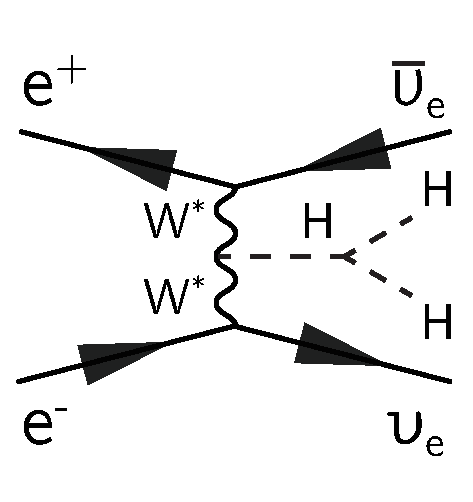
\includegraphics[width=\textwidth]{{{doubleHiggs/Feynman/1}}}
    \caption{}
    \label{fig:doubleHiggsFeynman1}
  \end{subfigure}
  \hfill
  \begin{subfigure}[b]{0.22\textwidth}
    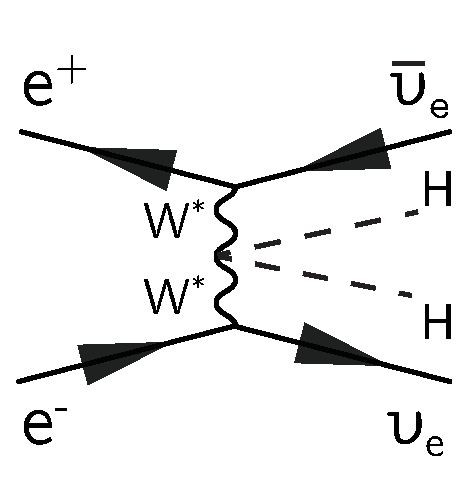
\includegraphics[width=\textwidth]{{{doubleHiggs/Feynman/2}}}
    \caption{}
    \label{fig:doubleHiggsFeynman2}
  \end{subfigure}
  \begin{subfigure}[b]{0.22\textwidth}
    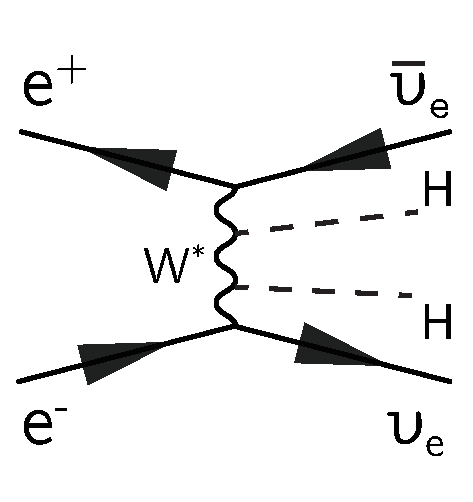
\includegraphics[width=\textwidth]{{{doubleHiggs/Feynman/3}}}
    \caption{}
    \label{fig:doubleHiggsFeynman3}
  \end{subfigure}
  \hfill
  \begin{subfigure}[b]{0.22\textwidth}
    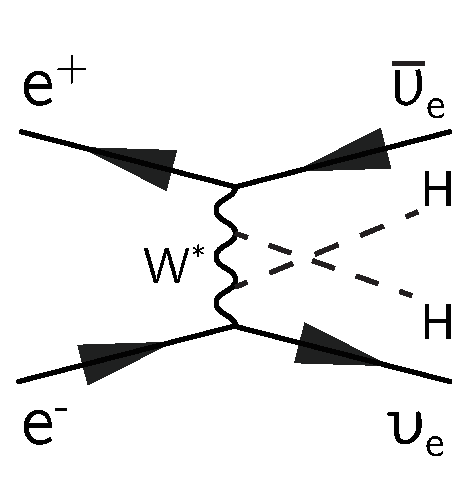
\includegraphics[width=\textwidth]{{{doubleHiggs/Feynman/4}}}
    \caption{}
    \label{fig:doubleHiggsFeynman4}
  \end{subfigure}
\caption
   {The main Feynman diagrams for the leading-order \eeToHH processes at the \CLIC.}
   \label{fig:doubleHiggsFeynman}
\end{figure}

Double Higgs production can be also produced via {\HepProcess{ \Pep \Pem \to \PZ \PHiggs \PHiggs}\xspace}, where \PZ decays to \HepProcess{\Pnu \APnu}. This \HepProcess{\PZ \PHiggs \PHiggs} channel has also been used for study at future \ee colliders, for example, the \ILC at \rootSGeV{500} \cite{Baer:2013cma}. However, for the relevant \CLIC energies of \rootS{1.4} and 3\,TeV, its contribution to the \HepProcess{\PHiggs \PHiggs \Pnu \APnu} final state is small compared to that of the \WW fusion, and can be neglected.

%The cross section of {\HepProcess{ \Pem \Pep \to \PZ \PHiggs \PHiggs}\xspace} is one order of magnitude smaller than \eeToHH via the \WW fusion,  shown in \Figure{fig:theoryHiggsCrossSection},. Therefore, the effect of {\HepProcess{ \Pem \Pep \to \PZ \PHiggs \PHiggs}\xspace} present in \eeToHH channel at \rootS{1.4} and 3\,TeV is negligible.


%However, {\HepProcess{ \Pem \Pep \to \PZ \PHiggs \PHiggs}\xspace} can be easily identified via the recoil mass. Hence {\HepProcess{ \Pem \Pep \to \PZ \PHiggs \PHiggs}\xspace} is not considered in this studied.

From an experimental prospective, the two Higgs in the  \eeToHH decay to a range of particles. Hence the double Higgs production has several distinct final-state topologies. The sub-channel with the largest cross section, \eeToHHbbbb, is studied by the collaborators in the \CERN. In this chapter, the \eeToHHbbWW sub-channel  is investigated. Firstly hadronic decay of the \WW in the \eeToHHbbWW channel is studied, because the hadronic decay has the largest cross section  in the \eeToHHbbWW channel . The hadronic decay sub-channel  does not have   neutrinos in the final state, which allows each \PW to be reconstructed. The semi-leptonic final state of the \WW system in the \eeToHHbbWW is also considered. The presence of the neutrino in the final state makes it  difficult to reconstruct the two Higgs bosons, as some momenta of one Higgs boson is carried by the neutrino. %This channel is discussed briefly and its analysis strategy is adapted from the hadronic decay analysis.
%The double Higgs production, \eeToHH, is divided into two sub-channel: \eeToHHbbWW and \eeToHHbbbb to target the specific kinematic properties if each final state, which provides cross-validation between two sub-channels and an improvement in signal selection when combined.


%However, hadronic decay final state of the \eeToHHbbWW has a very low cross section. The signal selection is challenging and aggressive background rejection methods are deployed.
%The analysis of the \eeToHHbbbb  sub-channel has been studied independently by collaborators. In this thesis, two analyses are combined for the final couplings extractions.
%The    is studied independently by collaborators. However, there is collaboration between the two studies. The two analyses are combined on the final couplings extractions.

%Combining with the low cross section, results for these two final states are not reported. The analysis can be easily (and have been) adapted for the semi-leptonic and leptonic final states.

The process, \eeToHHbbWWHadFull, results in a six quark final state with missing momentum. The high number of quarks requires an efficient jet reconstruction and a jet pairing algorithm to select the signal events. The two \Pbottom quarks in the final state can be identified statistically with \Pbottom jet tagging. %Since the final state does not contain leptons, event-level lepton finding - typically for energetic isolated leptons -  would improve the signal selection efficiency.

A fast simulation study of the double Higgs production has already been performed using the \CLICILD detector model for \rootS{1.4} and 3\,TeV\cite{Linssen:2012hp}. In this chapter a full \CLICILD detector simulation study is presented. Firstly, suitable signal and background channels are identified. In order to select the signal events, events with identified isolated lepton are vetoed.  Vertex information is used to identify \Pbottom quark jets. The \PFOs in an event are then clustered into jets depending on the number of quarks in the final states. The jets are then used as inputs for pre-selection and multivariate analysis. The event reconstruction was performed using the Marlin framework and reconstruction package in \ilcsoft v01-16. More details on the reconstruction software can be found in \Chapter{chap:Reconstruction}.



% The \eeToHHbbWW hadronic decay will be presented first, followed by the semi-leptonic sub-channel analysis.




\section{Monte Carlo sample generation}


% TODO
% Understand beamsstrahlung and EPA
For this simulation study, the first step is to generate Monte Carlo samples. A full list of generated samples with their cross sections can be found in \Table{tab:doubleHiggsMCSamples}. The software used  is described in \Section{sec:pandoraMC}.

At high centre-of-mass energies, in addition to considering electron-electron interactions, electron-photon and photon-photon interactions are important as their interactions become significant. These photons are produced due to the high electric field generated by the colliding beams. Processes involving real photons from beamsstrahlung (BS) and ``quasi-real'' photons are generated separately. For the ``quasi-real'' photon initiated processes, the Equivalent Photon Approximation (EPA) has been used \cite{lyth:jpa00215525}.

%Background samples considered in this analysis are listed in Table \ref{tab:doubleHiggsMCSamples}. The signal channel is \eeToHHbbWWFull where both \PW 's decay hadronically.
%W's decay hadronically? Does this make sense from a physics point of view?
%The analysis is performed with \CLICILD detector concept at \rootS{1.4} and 3\,TeV, and the semi-leptonic channel. Unless specified, the

Background processes with multiple quarks and missing momentum in the finial states are challenging to reject, as the topologies are similar to that of the signal events. Two example background processes are \eeTo{ \Pquark \Pquark \Pquark \Pquark \Pnu \APnu} and \HepProcess{\Pepm\Pphoton \to \Pnu \Pquark \Pquark \Pquark \Pquark}. For the same reason, single Higgs boson production, such as \eeTo{\Pquark \Pquark \PHiggs \Pnu \APnu}, has a similar final state to the signal events and it is also difficult to reject.

Some processes are not considered in this analysis because they either have very different event topologies to the signal, or they have very small cross sections. For example,  \HepProcess{\Egamma   \to \Pquark \Pquark \PHiggs \Plepton} is neglected  as the cross section is very small, even at \rootS{3}.

%For example, six-quark final states were not simulated due to constraints of the simulating software.
As the background processes are generated according to the final states. The final states of background processes could happen via Higgs production, which would result in double counting of Higgs events with signal sample.  Therefore to separate Higgs production from other processes, all background processes are generated with a Higgs boson mass of 14\,TeV to ensure a negligible Higgs contribution. Processes involving Higgs production are simulated with a Higgs boson mass of 126\,GeV.

The cross section of the signal, \eeToHHbbWW, is scaled according to values listed in \cite{Dittmaier:2012vm}, as the default Higgs branching ratios in the generator software are less accurate than the values listed in \cite{Dittmaier:2012vm}.

%Multi-quark final state background samples could, in principle, contain higgs production. Therefore, they are generated with a Higgs mass of 14\,TeV. This will

% ATTN need to rewrite
The simulation and reconstruction chain is described in \Chapter{chap:Reconstruction}. For some background processes, events are generated requiring the invariant mass of the total momenta of all quarks above 50\,GeV or 120\,GeV, because the invariant masses of the visible momenta of signal events are mostly above 150\,GeV.

%   For electron-photon interaction with $\Pquark\Pquark\Pquark\Pquark\Pnu$ final state at \rootS(1.4), events are simulated requiring invariant mass of quarks above 120\,GeV.

% These generator level cuts requires  limits are necessary to generate a large amount of background samples in a feasible timeframe, without losing significant signal samples.

Finally, the beam induced background \ggHad is simulated and overlayed on all events. Details can be found in \Section{sec:pandoraggHad}.
% according to the integration time of each subdetector

\begin{table}[!tbp]\centering
% TODO fix lumi correction for e gamma, gamma e
% TODO change some of sample cross section for  electron-photon interaction with four quarks and a neutrino final state

%{
\begin{tabular}{lr}
\hline \hline
Channel  &  $\sigma(\rootS{1.4})$ / fb   \\
\hline
\eeToHH & 0.149 \\
\hline
\eeToHHbbWWFull,hadronic & 0.018  \\
\eeToHHbbbbFull & 0.047 \\
\eeToHHotherFull & 0.085 \\
\hline
\eeTo{\qlight \qlight \PHiggs \Pnu \APnu}  & 0.86 \\
\eeTo{\Pcharm \APcharm \PHiggs \Pnu \APnu}  & 0.36 \\
\eeTo{\Pbottom \APbottom \PHiggs \Pnu \APnu}  & 0.31 \\

\eeTo{ \Pquark \Pquark \Pquark \Pquark}   &   1245.1\\
\eeTo{ \Pquark \Pquark \Pquark \Pquark \Plepton \Plepton}& 62.1* \\
\eeTo{ \Pquark \Pquark \Pquark \Pquark \Plepton \Pnu}& 110.4*\\
\eeTo{ \Pquark \Pquark \Pquark \Pquark \Pnu \APnu} & 23.2* \\

\eeTo{ \Pquark \Pquark} &  4009.5\\
\eeTo{ \Pquark \Pquark \Plepton \Pnu} &  4309.7\\
\eeTo{ \Pquark \Pquark \Pl \Pl} &  2725.8 \\
\eeTo{ \Pquark \Pquark \Pnu \Pnu} & 787.7  \\
\hline
\egamma{\Pepm}{\Pphoton}{\BS}{\Pepm \Pquark \Pquark \Pquark \Pquark} & 2317  \\
%\egamma{\Pem}{\Pphoton}{BS}{\Pem \Pquark \Pquark \Pquark \Pquark} & 1160.7  \\
%\egamma{\Pep}{\Pphoton}{BS}{\Pep \Pquark \Pquark \Pquark \Pquark} & 1156.3 \\
\egamma{\Pepm}{\Pphoton}{\EPA}{\Pepm \Pquark \Pquark \Pquark \Pquark} & 574 \\
%\egamma{\Pem}{\Pphoton}{EPA}{\Pem \Pquark \Pquark \Pquark \Pquark} & 287.1 \\
%\egamma{\Pep}{\Pphoton}{EPA}{\Pep \Pquark \Pquark \Pquark \Pquark}  & 286.9 \\
\egamma{\Pepm}{\Pphoton}{\BS}{\Pnu \Pquark \Pquark \Pquark \Pquark}& 159.1\myDagger \\
%\egamma{\Pem}{\Pphoton}{BS}{\Pnu \Pquark \Pquark \Pquark \Pquark}& 79.8\myDagger \\
%\egamma{\Pep}{\Pphoton}{BS}{\APnu \Pquark \Pquark \Pquark \Pquark}& 79.3\myDagger \\
\egamma{\Pepm}{\Pphoton}{\EPA}{\Pnu \Pquark \Pquark \Pquark \Pquark}& 34.7\myDagger  \\
%\egamma{\Pem}{\Pphoton}{EPA}{\Pnu \Pquark \Pquark \Pquark \Pquark}& 17.4\myDagger  \\
%\egamma{\Pep}{\Pphoton}{EPA}{\APnu \Pquark \Pquark \Pquark \Pquark}& 17.3\myDagger  \\
\egamma{\Pepm}{\Pphoton}{\BS}{\Pquark \Pquark \PHiggs \Pnu} & 31.5* \\
%\egamma{\Pem}{\Pphoton}{BS}{\Pquark \Pquark \PHiggs \Pnu} & 15.8* \\
%\egamma{\Pep}{\Pphoton}{BS}{\Pquark \Pquark \PHiggs \Pnu} & 15.7* \\
\egamma{\Pepm}{\Pphoton}{\EPA}{\Pquark \Pquark \PHiggs \Pnu} & 6.78* \\
%\egamma{\Pem}{\Pphoton}{EPA}{\Pquark \Pquark \PHiggs \Pnu} & 3.39* \\
%\egamma{\Pep}{\Pphoton}{EPA}{\Pquark \Pquark \PHiggs \Pnu} & 3.39*   \\
\hline
\gammagamma{\Pphoton}{\BS}{\Pphoton}{\BS}{ \Pquark \Pquark \Pquark \Pquark}& 21406.2*  \\
\gammagamma{\Pphoton}{\BS}{\Pphoton}{\EPA}{ \Pquark \Pquark \Pquark \Pquark}& 4018.7* \\
\gammagamma{\Pphoton}{\EPA}{\Pphoton}{\BS}{ \Pquark \Pquark \Pquark \Pquark}& 4034.8* \\
\gammagamma{\Pphoton}{\EPA}{\Pphoton}{\EPA}{ \Pquark \Pquark \Pquark \Pquark}& 753.0* \\
\hline \hline
\end{tabular}

\caption[Signal and background samples with the corresponding cross sections at \rootS{1.4}.]
{List of signal and background samples used in the double Higgs analysis with the corresponding cross sections at \rootS{1.4}. \Pquark can be \Pup, \Pdown, \Pstrange, \Pbottom or \Ptop. Unless specified, \Pquark, \Plepton and \Pnu represent either particles or the corresponding anti-particles. \Pphoton(BS) represents a real photon from beamstrahlung (BS). \Pphoton(EPA) represents a ``quasi-real'' photon, simulated with the Equivalent Photon Approximation. For processes labeled with * and $\myDagger$, events are generated with the invariant mass of the total momenta of all quarks above 50 and 120\,GeV, respectively.}
\label{tab:doubleHiggsMCSamples}
\end{table}
%Simulated \PW has invariant mass of 80.385\,GeV.

\section{Lepton identification}
\label{sec:doubleHiggsLepton}

For the signal channel, \eeToHHbbWWHad, there is no primary lepton in the final state, whilst many background  processes, such as \HepProcess{\Pquark \Pquark \Pquark \Pquark \Plepton \Pnu}, contain primary leptons in final states. Hence, efficiently rejecting events with primary leptons is an important step in the event selection. Primary leptons deposit energies in the tracking detector. The start of the energy deposition is typically very close to the interaction point. The primary leptons often have energies above 10\,GeV and are  isolated from other particles. Whilst electrons and muons are stable enough to deposit energies in the calorimeters, tau leptons are very short lived. With a typical decay lifetime of 290\,fs\cite{Abreu:1991jn,Agashe:2014kda}, it decays before reaching the vertex detector. Therefore, only decay products of the tau leptons can be reconstructed.


%New processors have been developed and existing processors have been optimised for signal selection and background rejection.
%The reconstruction is done via Marlin in \ilcsoft v01-16. The latest functioning flavour tagging processor exist in \ilcsoft v01-16. Thus newer versions of  \ilcsoft can not be used in this analysis.



\subsection{Electron and muon identification}
\label{sec:doubleHiggsLeptonID}

Two approaches to electron and muon identification were utilised, which are described below. The performance is summarised in \Table{tab:doubleHiggsIsoLepPerformance}.

%Two Marlin reconstruction for processors for light lepton(\Pe, \Pmu) tagging are used and optimised. As it is important to identify primary light leptons to help to select signal events, two additional light lepton tagging processors are developed and optimised.

 %described followed by their performances. As the signal is very rare comparing to the background, it is necessary to develop high performance isolated lepton finder to veto events with leptons and improve the signal selection efficiency. An existing lepton finder is optimised in \Section{sec:doubleHiggsIsolatedLeptonFinder} and a separate lepton finder is developed by the author in \Section{sec:doubleHiggsBonoLeptonFinder}.

\subsubsection{\IsolatedLeptonFinderProcessor}
\label{sec:doubleHiggsIsolatedLeptonFinder}
The \IsolatedLeptonFinderProcessor reconstruction package is used and optimised. This processor identifies high energy electrons and muons that are isolated from other particles. The algorithm parameters wer optimised using the signal channel and the \eeTo{ \Pquark \Pquark \Pquark \Pquark \Plepton \Pnu} channel, which is a multi-quark final state containing a primary lepton.

%Electron induced electromagnetic showers are mostly contained in the \ECAL. The primary electrons and muons from the electron-positron interaction leaves primary tracks in the tracking detector, which start typically less than 0.05\,mm from the interaction point. The isolation criteria requires the lepton to be spatially separated from other high energy particles.

Optimal values of the \IsolatedLeptonFinderProcessor are listed in \Table{tab:doubleHiggsIsolatedLeptonFinder}. $E$ is the energy of the lepton. $E_{\ECAL}$ is the energy of the lepton deposited in the \ECAL in GeV. $E_{cone}$ is the total energy within a cone of an opening angle of $\cos^{-1}(0.995)$ around the lepton, in GeV. $d_0$, $z_0$, and $r_0$ are the Euclidean distance in mm of the lepton track starting point to the interaction point in $x$-$y$ plane, in $z$ direction, and in $x$-$y$-$z$ three dimensional space, respectively.

\begin{table}[!htbp]
\begin{tabular}{lr}
\hline
\hline
\IsolatedLeptonFinderProcessor  & Selection \\
\hline
High Energy &  $E > 15$\,GeV  \\
\Pepm ID & $\frac{E_{\ECAL}}{E} > 0.9$ \\
\Pmupm ID &  $ 0.25> \frac{E_{ECAL}}{E} > 0.05$\\
Primary Track  & $d_0 < 0.02\,mm, z_0 < 0.03\,mm, r_0 < 0.04\,mm$ \\
Isolation & $E_{cone}^2 \leqslant 5.7 \times E - 50$ \\
\hline
\hline

\end{tabular}
\caption
{Optimised parameters of \IsolatedLeptonFinderProcessor}
\label{tab:doubleHiggsIsolatedLeptonFinder}
\end{table}

\subsubsection{\BonoLeptonFinder}
\label{sec:doubleHiggsBonoLeptonFinder}

A complimentary electron finder, \BonoLeptonFinder, is developed to further identify isolated electrons and muons. Compared to the \IsolatedLeptonFinderProcessor, the main difference is that the \BonoLeptonFinder utilises particle ID information provided by the \pandora to identify leptons.

%\IsolatedLeptonFinderProcessor has strict criterion to find high-energy isolated leptons to avoid mistakes. However, since the signal cross section is low in this analysis, it would be beneficial to reject more events with leptons identified to improve the signal to background ratio. Hence another isolated lepton finder is developed. The main feature of the \BonoLeptonFinder is that it utilises calorimetric information provided by \pandora.


The processor uses two sets of cuts to identify isolated leptons. If a PFO passes either set of cuts, it will be identified by the processor. The first set of cuts uses the particle ID information from \pandora, demanding a \pandora electron or muon with high \pT and the associated track depositing energy close to the interaction point. The identified lepton should either have a very high transverse momentum or be isolated. The second set of cuts uses \ECAL energy fraction, which for a PFO is the energy deposited in the \ECAL divided by the total energy, to determine the lepton ID. The rest of the cuts are very similar to the first cuts. The second set cuts have stricter isolation criterion to reduce fake rate.
%Not sure the last sentence above makes sense

\TABLE{tab:doubleHiggsBonoLeptonFinder} lists the  selection cuts for \BonoLeptonFinder. Same variables used in the \IsolatedLeptonFinderProcessor and the \BonoLeptonFinder are defined in the same way. \pT is the transverse momentum in GeV. $E_{cone1}$ and $E_{cone2}$ are the total energy of PFOs within a cone of an opening angle of $\cos^{-1}(0.995)$ and $\cos^{-1}(0.99)$ respectively around the lepton in GeV.


\begin{table}[!htbp]
\begin{tabular}{lr}
\hline
\hline
\BonoLeptonFinder  & Selection \\
\hline
High Energy &  $E > 10$\,GeV  \\
\Pepm ID & \pandora reconstructed \& $\frac{E_{\ECAL}}{E} > 0.95$ \\
\Pmupm ID &  \pandora reconstructed\\
Primary Track & $r_0 < 0.015$\,mm \\
a) High Transverse Momentum  &  $\pT > 40$\,GeV  \\
b) Isolation & $E \geqslant 23 \times \sqrt{E_{cone1}} + 5$ \\
\hline
High Energy  &  $E > 10$\,GeV  \\
\Pepm ID & $\frac{E_{\ECAL}}{E} > 0.95$ \\
\Pmupm ID & $0.2 > \frac{E_{\ECAL}}{E} > 0.05$ \\
Primary Track & $r_0 < 0.5$\,mm \\
a) High Transverse Momentum &  $\pT > 40$\,GeV  \\
b) Isolation & $ E \geqslant 28 \times \sqrt{E_{cone2}} + 30$ \\
\hline
\hline

\end{tabular}
\caption[Optimised parameters  of \BonoLeptonFinder.]
{Optimised parameters  of \BonoLeptonFinder. A PFO needs to pass either set of cuts to be identified as a lepton. Within a set of cuts, the PFO needs to satisfy either condition a) or b) to be identified as a lepton.}
\label{tab:doubleHiggsBonoLeptonFinder}
\end{table}


\begin{comment}
\subsubsection{Comparison: \IsolatedLeptonFinderProcessor versus \BonoLeptonFinder}

The two processors share similar criterion for light lepton identification. The main difference is that the \BonoLeptonFinder uses particle identification from \pandora, which takes into account extra calorimetric information to determine the particle ID than simple \ECAL energy fraction. \BonoLeptonFinder also allows high \pT light leptons to be identified in a non-isolated environment.
%aggressive nature of the \BonoLeptonFinder. %The performance of two processors on the signal and selected background samples is shown in \Table{tab:doubleHiggsIsoLepPerformance}.
\end{comment}

\subsection{Tau lepton identification}

Tau lepton has a short lifetime and decays before reaching the vertex detector. It can only be identified through the reconstruction of its decay products. The leptonic decay of tau lepton can be identified using the isolated lepton finder processors described above. Therefore in this section, tau identification will focus on the hadronic decays.

The existing \TauFinderProcessor  \cite{LCD-Note-2010-009} reconstruction package has been optimised. In addition, a package, \BonoTauFinder, is developed to provide additional tau lepton identification.

%To improve signal selection, a tau lepton identifier is developed by the author in \Section{sec:doubleHiggsBonoTauFinder}.



\subsubsection{\TauFinderProcessor}

The \TauFinderProcessor works by identifying tau lepton decay products, and requiring the decay products to be isolated from other PFOs. To find the decay products, the algorithm starts with the highest energy track selected as a seed for the cone clustering algorithm  (see  \Section{sec:pandoraConeCluster}). All tracks above 10\,GeV are iterated as seeds. A cone with opening angle 0.03 rad with respect to the seed is formed and the PFOs within the cone are required to be consistent with the signature of a tau hadronic decay. The signature includes no more than 3 charged particles in the cone, invariant mass less than 2\,GeV, and few than 10 \PFOs in the cone. The cone is also required to be isolated from other particles. To reduce fake rate, low momentum (less than 1\,GeV) and very forward particles ($\absOf{\cos\left(\theta_Z\right)} > 1.1$) do not participate in the tau finding, as they more likely come from \ggHad background.


The optimised parameters are listed in \Table{tab:doubleHiggsTauFinderProcessor}. Variables are defined in the same way as in previous sections. $\theta_Z$ is the polar angle with respect to the beam axis. $N_{X^+}$ and $N_{tau}$ are the number of charged particles and the number of \PFOs respectively in the tau cone. $m_{tau}$ is the invariant mass of the sum of the PFOs in the tau candidate in GeV. $E_{cone}$ is the total energy of \PFOs within a cone of an opening angle between 0.03 and 0.33\,rad  around tau seed in GeV.

\begin{table}[!htbp]
\begin{tabular}{lr}
\hline
\hline
\TauFinderProcessor  & Selection \\
\hline
Veto \ggHad  &  $\pT < 1$\,GeV, $\absOf{\cos\left(\theta_Z\right)} > 1.1$\,rad  \\
Seed particle & $\pT > 10$ \\
Tau candidate cone opening angle & 0.03\,rad \\
Tau candidate rejection & $N_{X^+} > 3$, $N_{tau} > 10$, $m_{tau} > 2$\,rad   \\
Isolation &  $ E_{cone} < 3$\,GeV\\
\hline
\hline
\end{tabular}
\caption
{Optimised parameters of \TauFinderProcessor.}
\label{tab:doubleHiggsTauFinderProcessor}
\end{table}

\subsubsection{\BonoTauFinder}
\label{sec:doubleHiggsBonoTauFinder}

The \BonoTauFinder works in a similar way as the \TauFinderProcessor. It identifies high momentum particles as tau seeds. Particles are iteratively added to a cone in the order of the ascending opening angle to the seed. The cone is called search cone, which contains tau decay products. After each particle addition, the temporary search cone is then considered as a temporary  tau candidate and tested for isolation and consistency  with a tau hadronic decay signature. The temporary tau candidate only needs to pass one of the isolation conditions to be identified as a tau candidate. There are multiple isolation conditions for tau 1-prong decay and 3-prong decay, reflecting different topologies of tau decay final states. The isolation criterion typically demand few particles around the search cone and the total \pT in the search cone to be greater than a threshold.

The iterative particle addition procedure stops when the cone opening angle is larger than a threshold. If multiple temporary tau candidates of the same tau seed pass the selection, the one with smallest opening angle is chosen to form the final tau candidate. To reduce fake tau decay products from \ggHad background, particles with energies less than 1\,GeV do not participate.


%tau hypothesis singular or tau hypotheses plural?


\TABLE{tab:doubleHiggsTauFinderProcessor} lists the optimised parameters  for \BonoTauFinder. Variables are defined in the same way as those in previous sections: $\theta_S$ is the opening angle of the search cone in rad; $cone1$ and $cone2$ are defined as a cone of an opening angle of $\cos^{-1}(0.95)$, and $\cos^{-1}(0.99)$ respectively around the tau seed; $r_0$ is the Euclidean distance in mm of the   tau seed associated track starting point to the interaction point in $x$-$y$-$z$ three dimensional space.

\begin{table}[!htbp]
\begin{tabular}{lr}
\hline
\hline
\BonoTauFinder  & Selection \\
\hline
Veto \ggHad&  $E < 1$\,GeV\\
Seed particle & $\pT > 5$\,GeV \\
Maximum search cone opening angle & $\theta_S \leqslant \cos^{-1}(0.999)$\,GeV\\
Tau candidate rejection & $N_{X^+} \neq 1,3$, $m_{PFO} > 3$\,GeV   \\
Isolation 1& $N_{cone1} = 0$, $ \pT_{cone} \geqslant 10$\,GeV\\
Isolation 2& $N_{X^+} = 1$, $N_{cone1} = 1$, $r_0 > 0.01$\,mm\\
Isolation 3& \multicolumn{1}{R{0.4\textwidth}}{{$N_{X^+} = 3$, $N_{cone1} = 1$, $ \pT_{cone} \geqslant 10$\,GeV, $\theta_S < \cos^{-1}(0.9995)$}}\\
Isolation 4& \multicolumn{1}{R{0.4\textwidth}}{$N_{X^+} = 1$, $N_{cone2} = 0$, $r_0 > 0.01$\,mm, $ \pT_{cone} \geqslant 10$\,GeV}\\
Isolation 5& \multicolumn{1}{R{0.4\textwidth}}{{$N_{X^+} = 3$, $N_{cone2} = 0$, $ \pT_{cone} \geqslant 10$\,GeV, $\theta_S < \cos^{-1}(0.9995)$}}\\
\hline
\hline

\end{tabular}
\caption
{Optimised parameters of \BonoTauFinder}
\label{tab:doubleHiggsBonoTauFinderProcessor}
\end{table}

Compared to the \TauFinderProcessor algorithm, the main difference is that the \BonoTauFinder has an iterative approach to build up a tau candidate, which allows a dynamic tau search cone size. The \BonoTauFinder also has smaller cut values on minimum \pT and invariant mass, but stricter isolation criterions.
%I've reworded the first sentence in this para - does it make sense?
%looser cut - is this the accepted term? if not, maybe replaced the word looser with something else

\subsection{Very forward electron identification}
\label{sec:doubleHiggsForwardElectron}

At the high centre-of-mass energy at the \CLIC, particles are often boosted.  It is important to identify leptons in the forward calorimeters to aid the signal selection because  certain background channels, for example photon-electron interactions, can have energetic primary  electrons in  the forward calorimeters, the \LumiCAL and/or the \BeamCAL.

It is challenging to identify electrons in these forward calorimeters.  Most particles in these forward calorimeters are from the beam induced background. Nevertheless, sufficiently high energy electrons can be efficiently identified in the \BeamCAL   and \LumiCAL \cite{sailer2012radiation}.
\begin{comment}
The high charge density in the bunches will induce strong electromagnetic fields causing deflection of the
beam particles and the radiation of
beamstrahlung
. In addition, the beamstrahlung photons will interact
with the beam particles and produce electron–positron and quark–anti-quark pairs.  While the photonic
component will be radiated practically along the outgoing beam axis, a noticeable fraction of leptonic
and hadronic pairs will hit the BeamCal calorimeter in the forward region.
\end{comment}

The reconstruction of electrons in the forward calorimeters uses  a parametrisation approach.  By parameterising the  particle ID efficiency using MC particles, the equivalent performance to the full detector simulation approach can be achieved \cite{Sailer:2017onh,Lukic:forwardElectron} .

%For the \CLICILD detector concept, energies deposited in the \LumiCAL and the \BeamCAL are not reconstructed in simulation. This is because the thousands of beam induced background particles per bunch crossing requires expensive computational resources. However, previous studies \cite{Sailer:2017onh,Lukic:forwardElectron} using parameterise the particle ID efficiency using MC particles give equivalent performance to the full detector simulation approach.


%The current simulation software could not handle the simulation in a feasible time. Therefore, the adopted approach is to parameterise the background particle energy deposition leading to electron tagging algorithms.
%I changed 'and leads to' to 'leading to'. Is that what you meant? The original text was mixing tenses

For the \BeamCAL, an existing electron tagging algorithm was developed using \rootS{3} collision environment by comparing the simulated electron and background energy distributions \cite{Sailer:2017onh}. An indicative performance plot of 500\,GeV electron tagging efficiency as a function of polar angle is shown in \Figure{fig:doubleHiggsForwardBCAL}. An electron is tagged if the energy is significantly larger than the expected background energy distributions integrated over 40 bunch crossing.

This parametric tagging approach  most likely underestimates efficiencies due to the coarse binning of energies. I.e. a 650\,GeV particle is treated the same as a 600\,GeV particle, as the tagging efficiency for electrons with energy 500 to 1500\,GeV are binned in histograms at an interval of 100\,GeV. Also there is no tagging efficiency for electrons with energy below 500\,GeV or about 1500\,GeV.


%A C++ code library has been developed and used in this analysis.

The input of the \BeamCAL electron tagging algorithm is the four momenta of the MC electron. Since the algorithm assumes collisions at \rootS{3}, for the \rootS{1.4} user case, the momenta of the MC electron is scaled down by a factor of $\frac{3}{1.4}$.



For the \LumiCAL,  \Figure{fig:doubleHiggsForwardCAL} shows the \LumiCAL  electron tagging efficiency as a function of the electron energy for polar angle $\theta = 50\,mrad$ where events are overlaid with background energy deposition integrated over 100 bunch crossings \cite{Lukic:forwardElectron}. In this analysis, the \LumiCAL electron tagging efficiency, $\varepsilon$, is parameterised as

%Assuming that the \LumiCAL electron tagging efficiency in this analysis is the same as in \Figure{fig:doubleHiggsForwardCAL} for all polar angles and for \rootS{1.4} and 3\,TeV,
%The \LumiCAL electron tagging in this analysis is based on the performance plot in \Figure{fig:doubleHiggsForwardCAL}.

%the \HepProcess{\PHiggs \to \Pmu \Pmu} analysis in \cite{Milutinovic-Dumbelovic:2014uta,Grefe:2012rt} has developed an algorithm for electron tagging in the \LumiCAL with similar logic to the algorithm for the \BeamCAL.
% as this is the only study available for comparison.


\begin{equation}
\varepsilon=
\begin{cases}
  0, & \text{if}\ E < 50\,GeV,\\
  0.99 \times \frac{(erf(E - 100) + 1 )}{2}, & \text{otherwise},
\end{cases}
\end{equation}
where $E$ is the energy of the electron and $erf$ is the error function. For each MC electron in the \LumiCAL, a random number between 0 and 1 is generated. If the random number is less than \varepsilon the MC electron is tagged.

%(see \Table{tab:detectorForwardILDvsCLICILD} for detector coverage)
Due to lack of tracking ability in the forward region, energy depositions from electrons or photons can not be differentiated in forward calorimeters. Therefore, both photons and electrons are tagged by the algorithms above.

\begin{figure}[!tbp]
  \begin{subfigure}[b]{0.45\textwidth}
    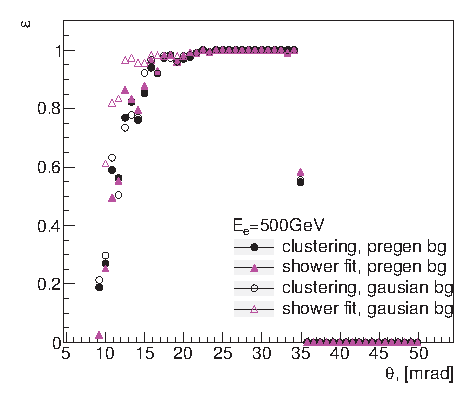
\includegraphics[width=\textwidth]{{{doubleHiggs/forward/ForwardBCAL}}}
    \caption{}
    \label{fig:doubleHiggsForwardBCAL}
  \end{subfigure}
  \hfill
  \begin{subfigure}[b]{0.45\textwidth}
    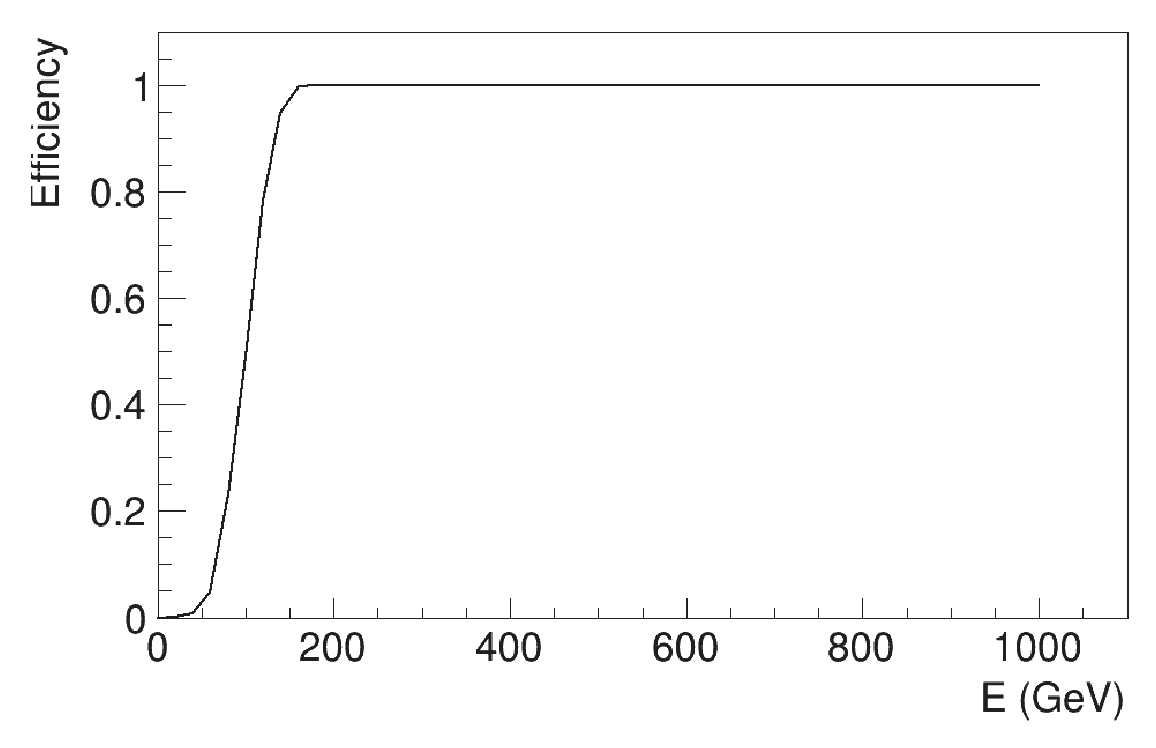
\includegraphics[width=\textwidth]{{{doubleHiggs/forward/ForwardLCAL}}}
    \caption{}
    \label{fig:doubleHiggsForwardLCAL}
  \end{subfigure}
\caption[\BeamCAL and \LumiCAL electron tagging efficiency.]%
   {\FIGURE{fig:doubleHiggsForwardBCAL} shows  500\,GeV electron tagging efficiency in the \BeamCAL as a function of polar angle, with different methods to model backgrounds: pregenerated and Gaussian,  and two methods to identify electrons:  clustering algorithm and  shower fitting algorithm, taken from \cite{Sailer:2017onh}. \FIGURE{fig:doubleHiggsForwardLCAL} shows the  electron tagging efficiency in the \LumiCAL as a function of the electron energy, for polar angle $\theta = 50\,mrad$, taken from \cite{Lukic:forwardElectron}. }
   \label{fig:doubleHiggsForwardCAL}
\end{figure}

%appear indistinguishable to the \BeamCAL and \LumiCAL and both photons and electrons are tagged by the above algorithms.


 %Due to the lack of tracking in these region, electrons and photons would have the same electromagnetic shower profile, with the given calorimeter resolution. MC photons and electrons are checked if they fall in the LCal or the BCal, and checked against the known detection efficiency.


%With the increase of the centre-of-mass energy, more  As discussed before, veto events with leptons help the signal selection. Hence the goal is to identify leptons in the forward region.

%These forward calorimeters were not simulated due to computational limitation.
% For \rootS(3), the BeamCal detection efficiency is provided by a software package \cite{}. For \rootS(1.4), the same software for the BeamCal is used, by scaling the energy of the MC particle by a factor of $\frac{3}{1.4}$. For the LumiCal, the identification efficiency is defined as


\subsection{Lepton identification performance}

The performances of the different lepton finding processors for signal events and the selected background processes are shown in \Table{tab:doubleHiggsIsoLepPerformance}. Numbers in the table  represent the fractions of events  where no leptons are identified by the individual lepton finder.  \BonoLeptonFinder and \BonoTauFinder reject more background events than the \IsolatedLeptonFinderProcessor and \TauFinderProcessor. By combining the processors, 86.6\% of the signal events remain and 16.8\% of the \HepProcess{\Pep \Pem \to \Pquark\Pquark\Pquark\Pquark\Plepton\Pnu} events survive after rejecting events where leptons are identified.
%Second sentence: can you say "" becase this would read better

The forward lepton finders are most effective at rejecting background events with primary leptons in the forward region. \TABLE{tab:doubleHiggsIsoLepPerformance} shows the performance of the processors with the signal events and the  \egamma{\Pem}{\Pphoton}{BS}{\Pem \Pquark \Pquark \Pquark \Pquark} background events. 53.6\% of the \egamma{\Pem}{\Pphoton}{BS}{\Pem \Pquark \Pquark \Pquark \Pquark} background events survive after rejecting events with leptons identified by the forward lepton finder. The full list of fraction of events  after rejecting events with leptons identified by any lepton finders for individual channel can be found in \Table{tab:doubleHiggs1.4TeVPreslection}.

\begin{table}[!tbp]
\begin{tabular}{lrrr}
\hline
\hline
Efficiency (1.4\,TeV)  &  Signal & \HepProcess{\Pep \Pem \to \Pquark\Pquark\Pquark\Pquark\Plepton\Pnu} & \egamma{\Pem}{\Pphoton}{\BS}{\Pem \Pquark \Pquark \Pquark \Pquark} \\
\hline
\IsolatedLeptonFinderProcessor & 99.3\% & 50.3\%  & 87.3\% \\
\BonoLeptonFinder & 99.1\% & 39.9\%  & 83.7\%\\
\TauFinderProcessor & 97.5\% & 52.3\%  & 90.4\% \\
\BonoTauFinder & 89.7\% & 38.5\%  &  78.5\% \\
Forward Finder Processors & 98.9\% & 95.1\%  & 53.6\% \\
\hline
Combined & 86.6\% & 16.8\%  &  30.8\% \\
\hline
\hline

\end{tabular}
\caption{The performances of  lepton finders on the signal events and selected background events at \rootS{1.4}.  Numbers represent the fractions of events where no leptons are identified by the individual lepton finder.}
\label{tab:doubleHiggsIsoLepPerformance}
\end{table}


The lepton finding processors are optimised with events at \rootS{1.4}, and checked with events at \rootS{3}.  It was found that the same set of parameters for lepton identifiers works well under \rootS{1.4} and 3\,TeV. The performances of the lepton finders with the signal and selected background events at \rootS{3} are shown in \Table{tab:doubleHiggs3TeVIsoLepPerformance}.

%Would this read better if you explained why 1.4 is better rather than why 3 is worse? Better should be the focus, no?
When comparing the lepton finding performances at \rootS{1.4} and \rootS{3}, the performance for \rootS{1.4} is better. This is because at \rootS{3}, particles are often boosted and spatial separation between particles is smaller. Therefore particles are less isolated from each other. The higher centre-of-mass at \rootS{3} also affects on the performance of the forward lepton finder. Whilst at \rootS{1.4}, the forward finder only rejects 5\% of the \HepProcess{\Pep \Pem \to \Pquark\Pquark\Pquark\Pquark\Plepton\Pnu} background events and 1\% of the signal events, at \rootS{3} it rejects 19\% of events from the same background process and 4\% of the signal events, as more leptons are boosted into the forward region.


\begin{table}[!tbp]
\begin{tabular}{lrrr}
\hline
\hline
Efficiency (3\,TeV)  &  Signal  & \HepProcess{\Pep \Pem \to \Pquark\Pquark\Pquark\Pquark\Plepton\Pnu}  & \egamma{\Pem}{\Pphoton}{\BS}{\Pem \Pquark \Pquark \Pquark \Pquark}  \\
\hline
\IsolatedLeptonFinderProcessor & 99.5\% & 66.8\% & 88.8\%  \\
\BonoLeptonFinder & 99.0\% & 52.5\%  & 82.2\%\\
\TauFinderProcessor & 97.7\% & 79.5\%  & 76.7\%\\
\BonoTauFinder & 86.3\% & 60.3\%  & 92.6\% \\
Forward Finder Processors & 95.9\% & 80.7\%  & 55.4\%  \\
\hline
Combined & 81.0\% & 23.3\% &  33.4\% \\
\hline
\hline

\end{tabular}
\caption{The performances of  lepton finders on the signal events and selected background events at \rootS{3}.  Numbers represent the fractions of events where no leptons are identified by the individual lepton finder.}
\label{tab:doubleHiggs3TeVIsoLepPerformance}
\end{table}


\begin{comment}
\begin{table}[!tbp]
\begin{tabular}{lrr}
\hline
\hline
Selection / Efficiency (1.4\,TeV)  &  Signal & \egamma{\Pem}{\Pphoton}{BS}{\Pem \Pquark \Pquark \Pquark \Pquark}  \\
\hline
Combined light lepton finder & 87.6\% & 67.5\%  \\
Forward Finder Processors & 98.9\% & 53.6\%  \\
\hline
Combined & 86.6\% & 30.8\%  \\
\hline
\hline

\end{tabular}
\caption{Very forward electron and photon finder performance on the signal and selected background events at \rootS{1.4}.}
\label{tab:doubleHiggsForwardPerformance}
\end{table}


\subsection{Other lepton identification processors}


Other isolated lepton identification processors have been tested, including IsolatedLeptonTagging and TauJetClustering. They either performed poorly comparing to the processors above, or became redundant after using the processors above. Therefore, these lepton identification processors are not used in this analysis.
%ATTN: does calibration/optimisation work better than tuning parameters?
\end{comment}

\section{Jet reconstruction}

Another important aspect of this analysis is to pair jets to reconstruct the physical bosons. The signal channel, \eeToHHbbWWHad, results in a six quark final state.  In this section, the optimisation of the jet reconstruction is discussed.



% A useful technique for the analysis is to reconstruct the multi-jet final state using jet algorithms. This allows discriminative variables to be calculated. A brief discussion about jet algorithms and its relevance for the \CLIC and this analysis are provided.

\subsection{Jet reconstruction optimisation}
\label{sec:doubleHiggsJetOptimisation}

Jet reconstruction algorithms cluster particles into jets. For this analysis, longitudinal invariant, \kt, jet algorithm is chosen for the jet clustering, as discussed in \Section{sec:pandoraJetAlg}. The free parameter for \kt algorithm is the $R$ parameter, which controls the radius of the jet. Another choice affecting the jet reconstruction is the choice of the \PFO collection, which incorporates different level of timing and \pT cuts to reduce the beam induce background (see \Section{sec:pandoraggHad}).
%Both parameters are optimised for \rootS{1.4} and \rootS{3}.

The value of the $R$ parameter and the \PFO collection are chosen to optimise the invariant mass and mass resolution of \PHiggs and \PW. To choose the optimal parameters, \eeToHHbbWWHad events  are processed through \kt jet algorithm  in the 6-jet exclusive mode. The six jets are paired using the MC truth information (see \Section{sec:pandoraMCtruthLink}) by examining the decay chain of MC particles. Four invariant mass distributions are obtained: two Higgs masses ($m_{\Hbb}$ and $m_{\HWW}$) and two \PW masses ($m_{\PW}$ and $m_{\W*}$). Here \W* indicates the off-mass-shell \PW boson.

%The metric for optimising the $R$ parameter, and the \PFO collection, is the invariant mass and mass resolution of \PHiggs and \PW. An optimised jet reconstruction is chosen such that invariant masses of \PHiggs and \PW are close to their true masses, and invariant mass widths are small.

%For the jet reconstruction optimisation, only signal events are used and jets are paired to using MC truth information (see \Section{sec:pandoraMCtruthLink}).

%The sample for the optimisation is \eeToHH.

%The signal channel, hadronic decay of , is used for the jet reconstruction optimisation. The signal
%The six jets are paired up using  MC truth information to the corresponding Higgs and \PW boson.
%I'm not sure this last sentence is worded correctly. Doesn't make sense to me but I'm not a physicist!

%An example of $m_{\Hbb}$ invariant mass distribution is shown in .  Although the underlying mass distribution of particles like $m_{\PW}$ is a Breit-Wigner distribution, the overall mass distribution is Gaussian like, as the overall mass distribution is a convolution of a narrow \PW Breit-Wigner distribution and a wide Gaussian distribution for the detector resolution. The $m_{\Hbb}$  mass distribution is gaussian like but with asymmetrical width, due to \Pbottom quarks decaying to neutrinos, leading to a loss of detectable particles.
%\paragraph{Mass resolution fit}
Three invariant mass distributions are considered:  $m_{\Hbb}$, $m_{\HWW}$, and $m_{\PW}$. The optimal jet reconstruction should produce a sharp mass peak around the simulated particle masses (see \Section{sec:pandoraCLICsimMass}). For example, \Figure{fig:doubleHiggsFitMCMass} shows the $m_{\Hbb}$ invariant mass distribution for $R = 1.3$ using the loose \PFO collection for samples at \rootS{3}. An analytical functional form is fitted to quantitatively describe the shape. The fitting function is a Gaussian-like function. Free parameters are used in the fitting function to fit the tail distribution. The fitting function takes the form of
\begin{equation}
f(m)=A e^{- \frac{(m - \mu)^2}{g}}
\end{equation}
\begin{equation}
g=
\begin{cases}
2\sigma_L + \alpha_L(m - \mu), & \text{if}\ m < \mu,\\
2\sigma_R + \alpha_R(m - \mu), & \text{if}\ m \geqslant \mu,
\end{cases}
\end{equation}
where: $\mu$ is the fitted mass peak position; $\sigma_L$ and $\sigma_R$ allow an asymmetrical width of the distribution; $\alpha_L$ and  $\alpha_R$  fit the tail of the distribution; and $A$ is the normalisation factor.


\begin{figure}[!htbp]
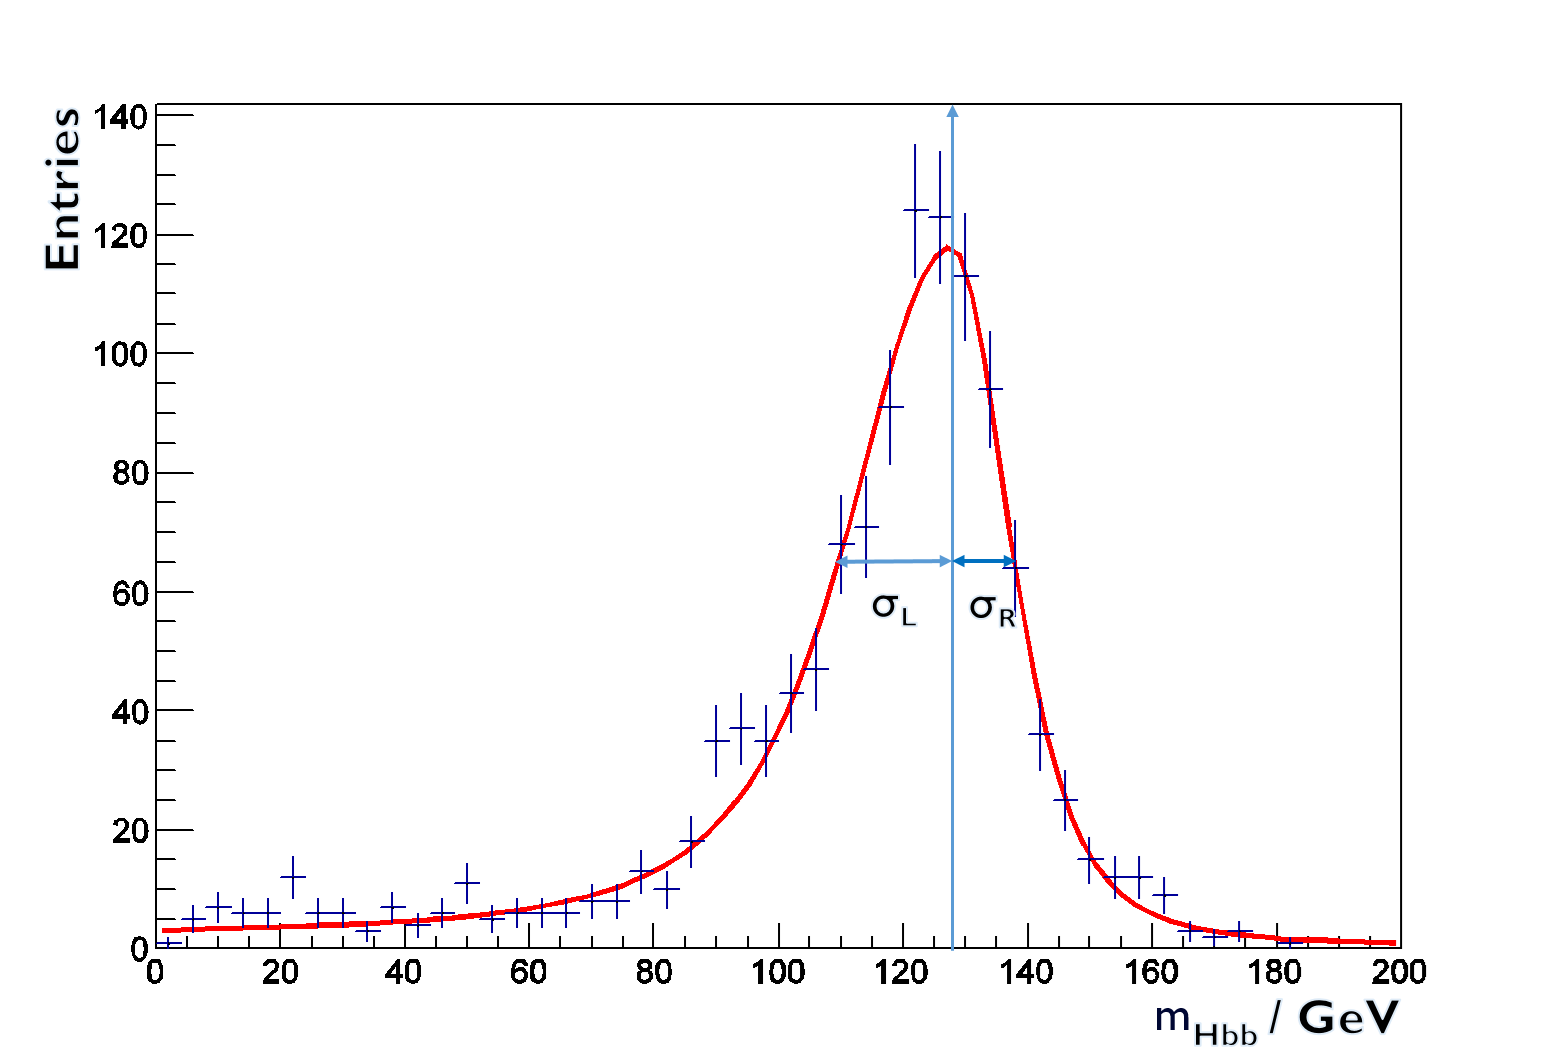
\includegraphics[width=\largefigwidth]{doubleHiggs/MCmassFit2}
\caption[Example MC mass fit for jet optimisation in double Higgs analysis]%
   {A typical example of  $m_{\Hbb}$  mass distribution with the superimposed fitting function in red. The arrow shows the fitted mean peak position.}
   \label{fig:doubleHiggsFitMCMass}
\end{figure}

%\paragraph{Optimal $R$ and \PFO collection}

%The mass fit is performed for $m_{\Hbb}$, $m_{\HWW}$, and $m_{\PW}$ distributions.  The optimal jet reconstruction should have the mass peak close to the particle's simulated mass and a narrow peak width.
The overall relative width is defined as $\left(\sigma_L  + \sigma_R\right)/M$. A smaller width indicates better a mass resolution. The fitted \Hbb, \HWW, and \PW masses are studied for $R$ values between 0.5 and 1.3, at interval of 0.1, and with three \PFO collections: loose, normal, and tight.


\FIGURE{fig:doubleHiggs1.4TeVMassFit} shows the variation of the mass peak position and the relative width as a function of $R$ and \PFO collections, for $m_{\Hbb}$, $m_{\HWW}$, and $m_{\PW}$. The mass peak position, $\mu$, increases as $R$ increases. This is because more particles are included in jets with increasing jet radius. For the relative width, the values for \Hbb  increase with increasing jet radius, but the values for \HWW decrease  with increasing jet radius. This is due to a compensating effect. The invariant mass for \HWW is formed from four jets, which prefers a large jet radius. The invariant mass for \HWW is obtained from two jets, which favours a small jet radius.

The choice of \PFO collection impacts number of \PFOs in the event. The loose \PFO selection has the most \PFOs in the event and, therefore, the largest invariant mass and worst mass resolution.

Based on the results summarised in \FIGURE{fig:doubleHiggs1.4TeVMassFit}, it was decided to use  $R = 0.7$  with the \normalPFO for this analysis. This choice  gives good fitted mass peak positions for \Hbb, \HWW and \PW. The extracted fitted parameters of optimal jet reconstructions are summarised in \Table{tab:doubleHiggsFitParameters}.

\begin{figure}[!tbp]
  \begin{subfigure}[b]{0.45\textwidth}
    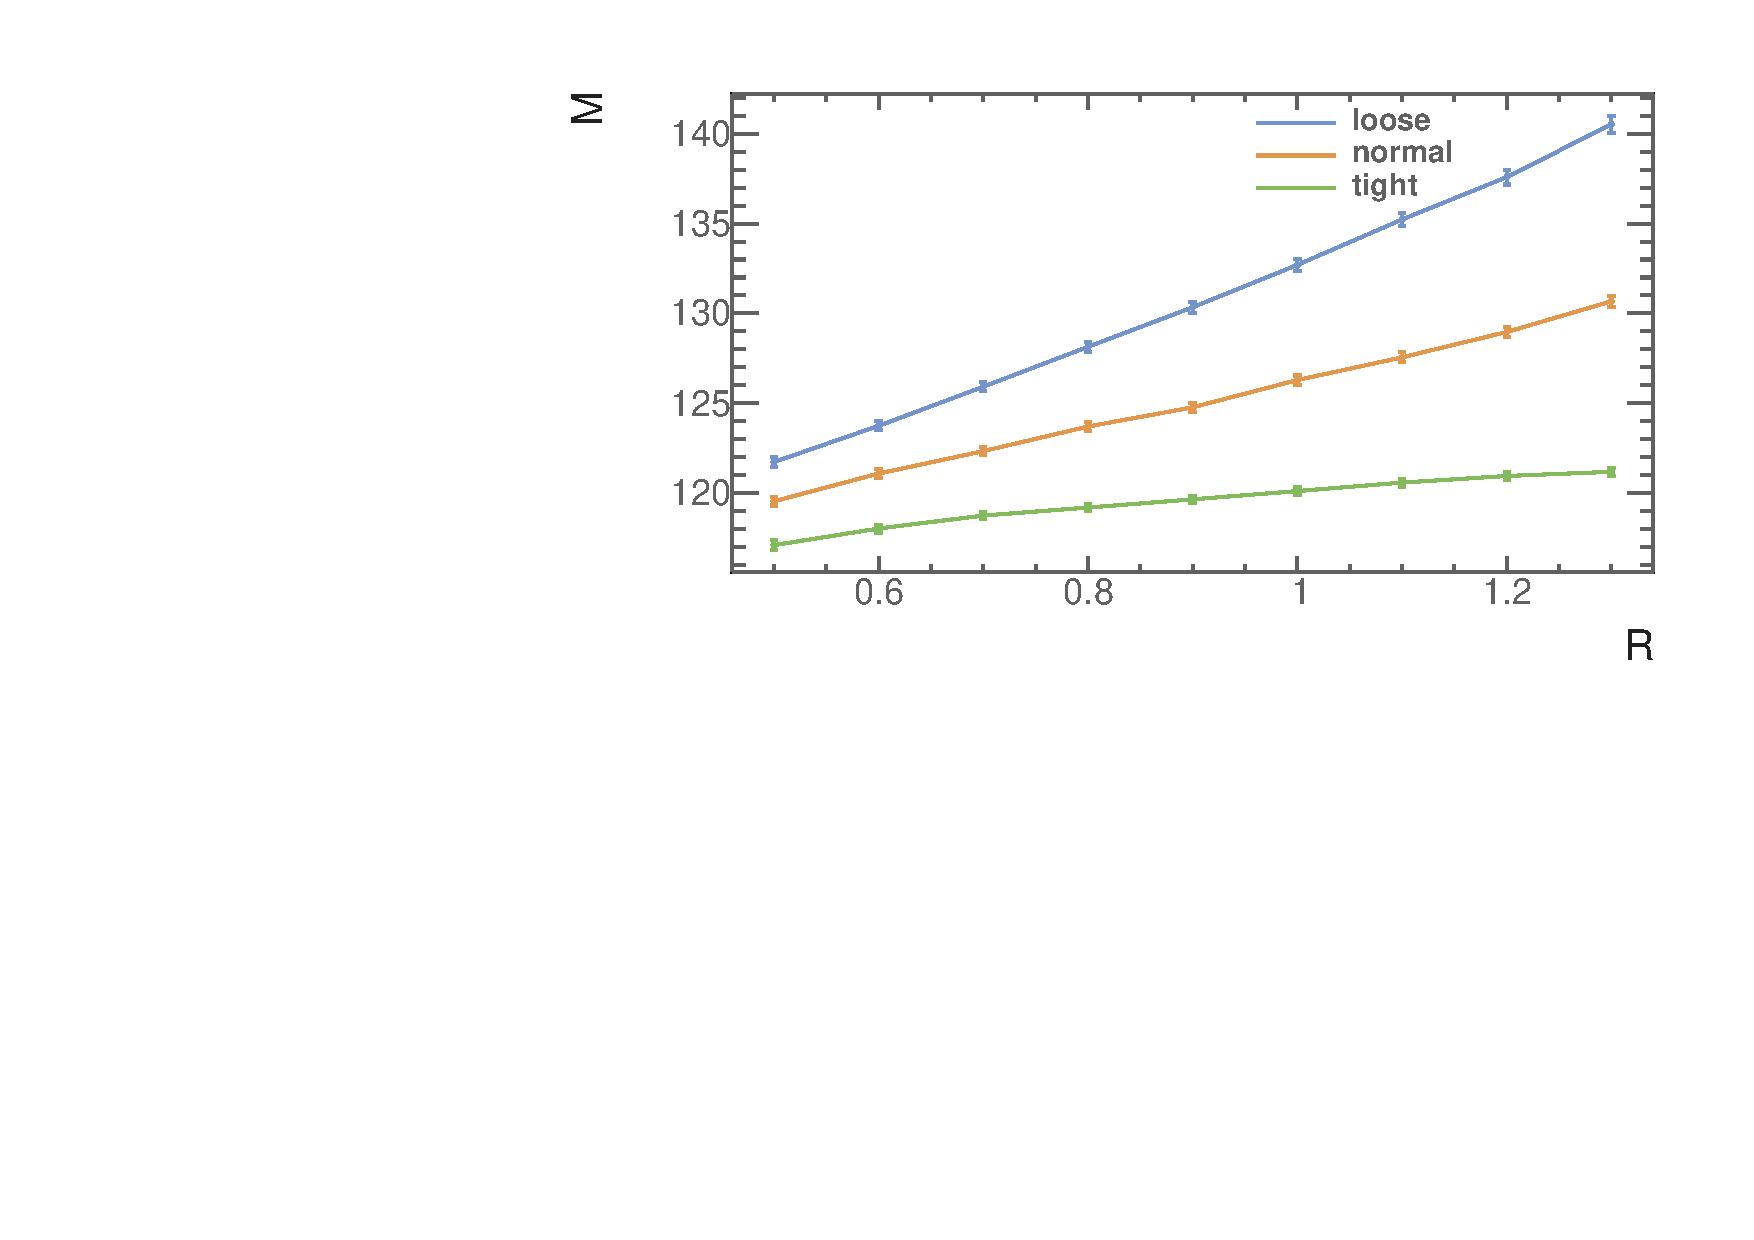
\includegraphics[width=\textwidth]{{doubleHiggs/resolution/ILD_1.4TeV_Higgs1_M_R}.pdf}
    \caption{}
    \label{fig:doubleHiggs1.4Higgs1M}
  \end{subfigure}
  \begin{subfigure}[b]{0.45\textwidth}
    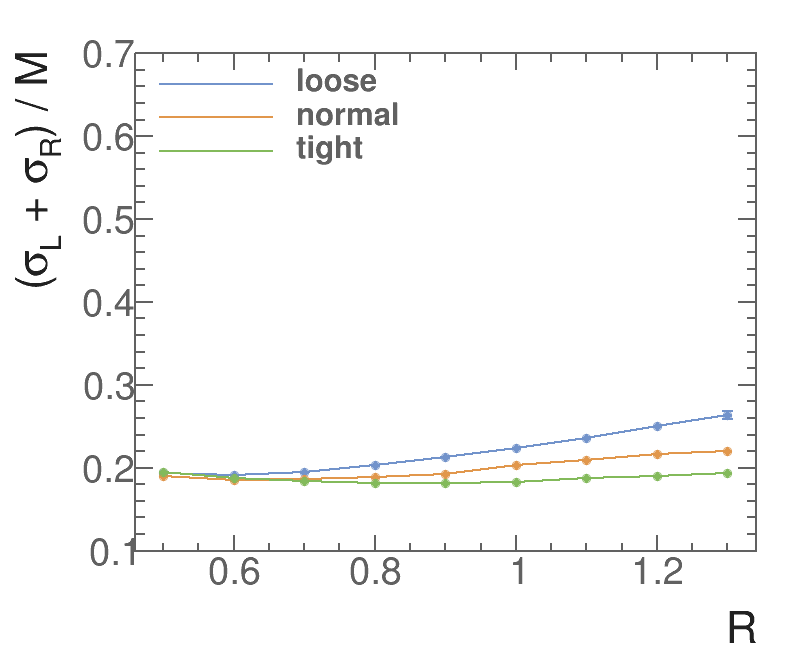
\includegraphics[width=\textwidth]{{doubleHiggs/resolution/ILD_1.4TeV_Higgs1_SigmaL_add_SigmaR_divide_M_testR}.pdf}
    \caption{}
    \label{fig:doubleHiggs1.4Higgs1Sigma}
  \end{subfigure}
  \begin{subfigure}[b]{0.45\textwidth}
    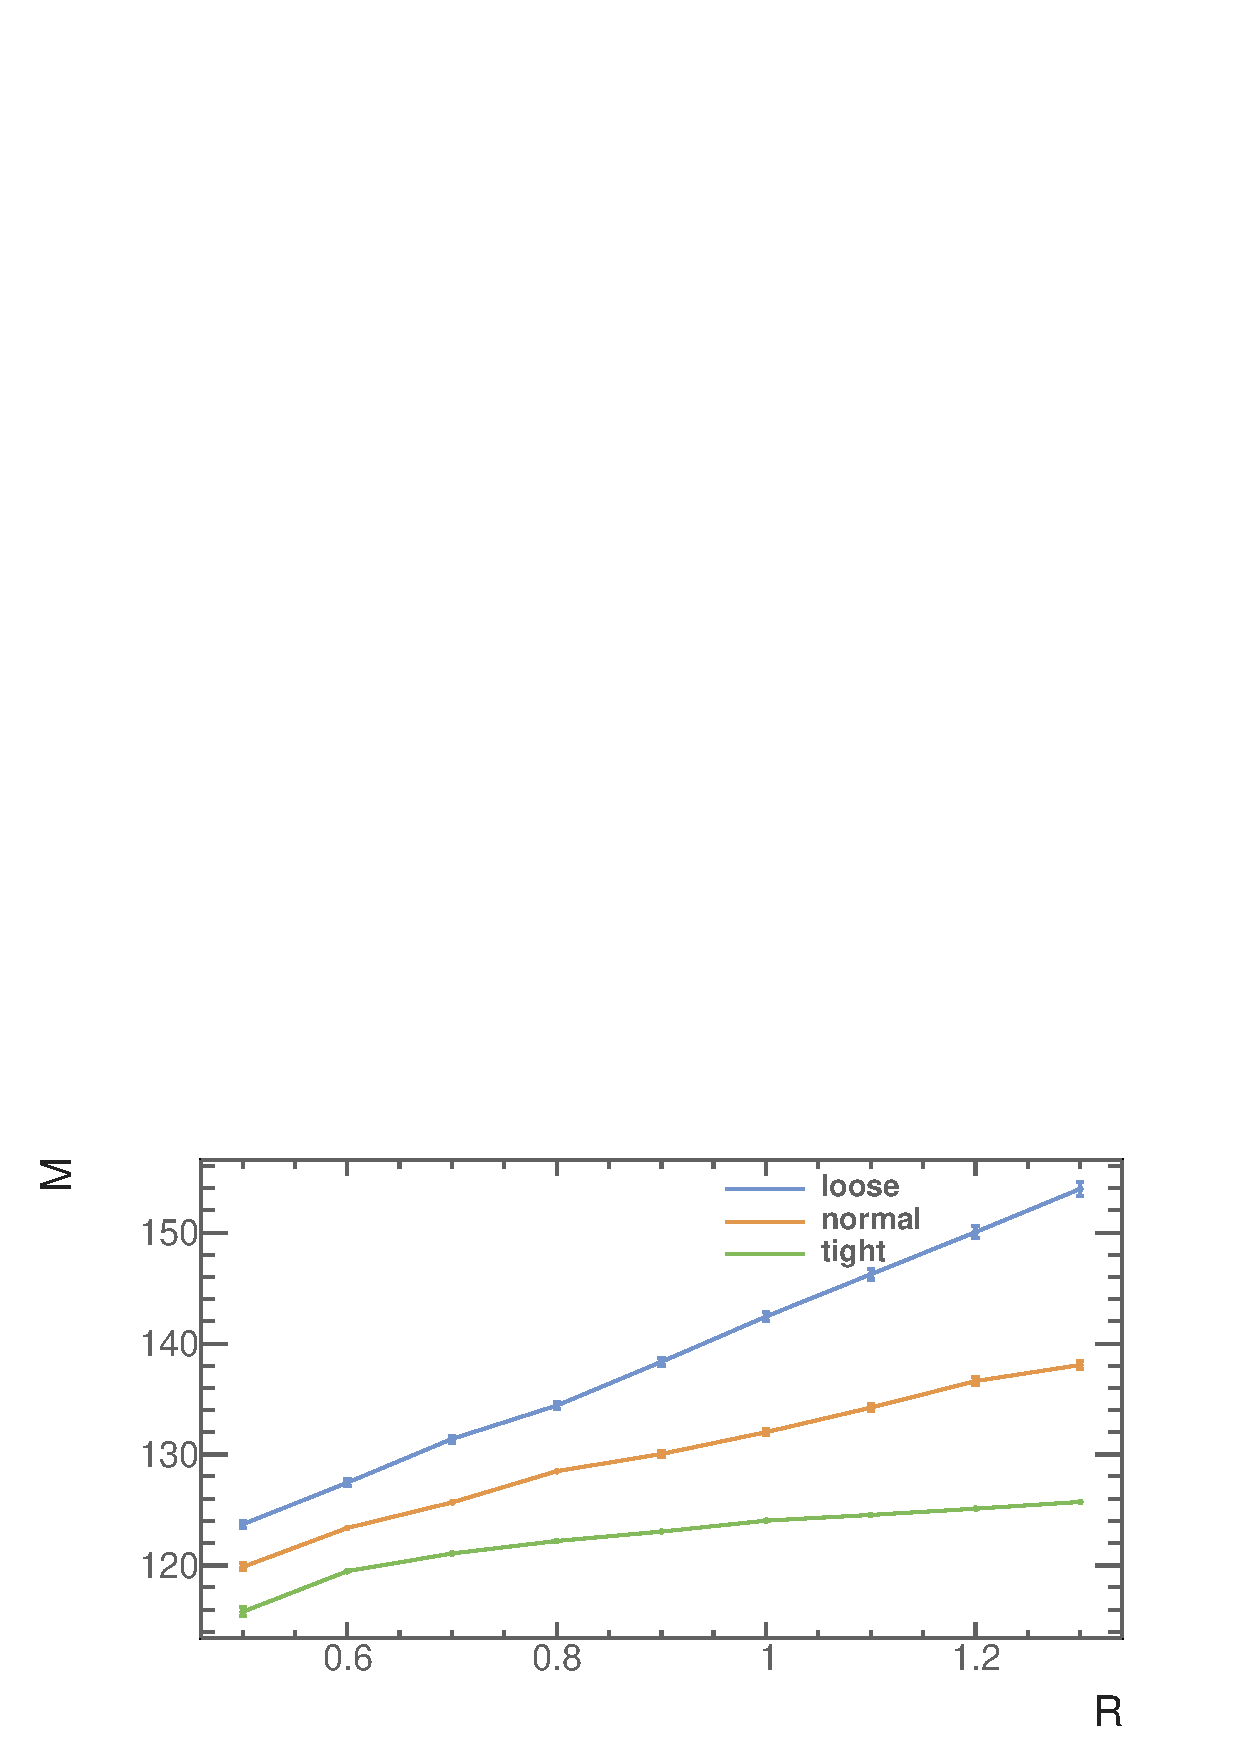
\includegraphics[width=\textwidth]{{doubleHiggs/resolution/ILD_1.4TeV_Higgs2_M_R}.pdf}
    \caption{}
    \label{fig:doubleHiggs1.4Higgs2M}
  \end{subfigure}
  \begin{subfigure}[b]{0.45\textwidth}
    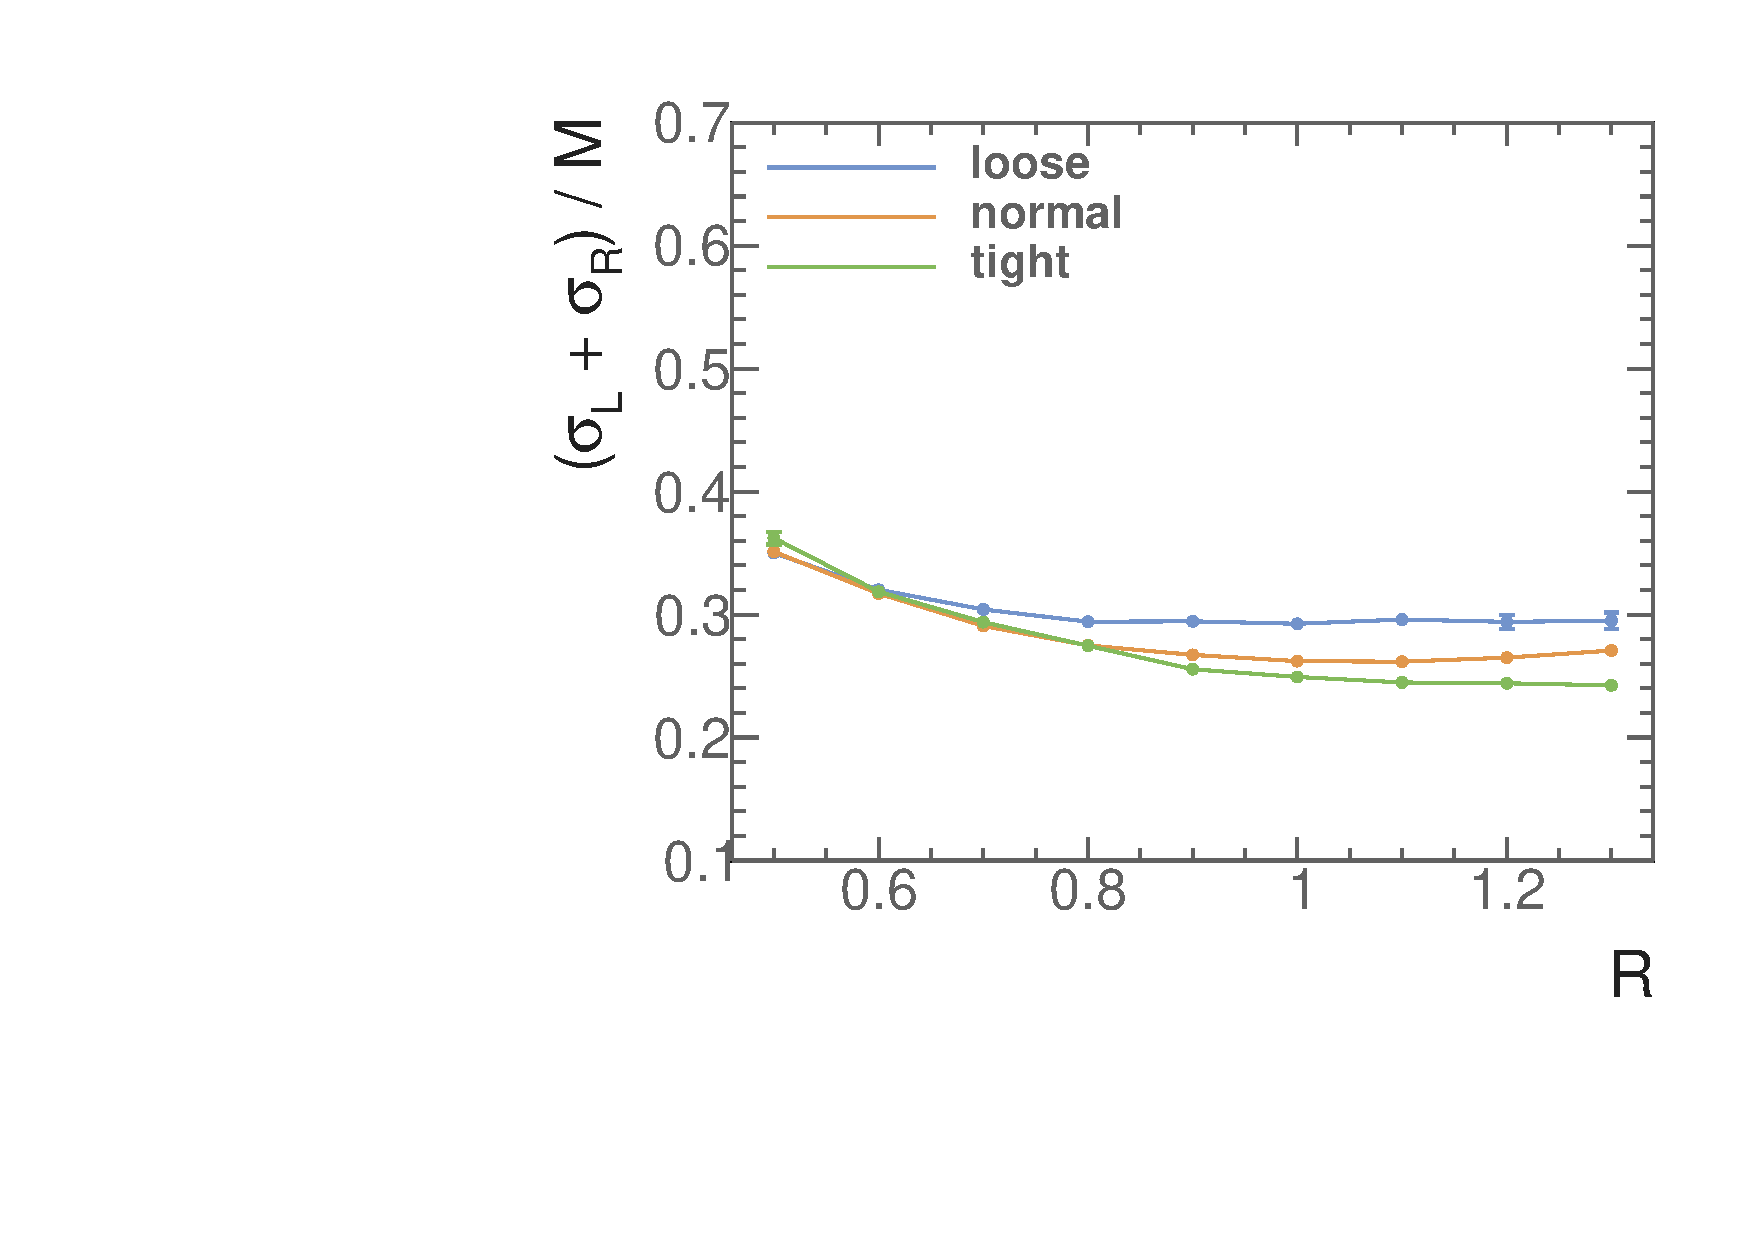
\includegraphics[width=\textwidth]{{doubleHiggs/resolution/ILD_1.4TeV_Higgs2_SigmaL_add_SigmaR_divide_M_testR}.pdf}
    \caption{}
    \label{fig:doubleHiggs1.4Higgs2Sigma}
  \end{subfigure}
  \begin{subfigure}[b]{0.45\textwidth}
    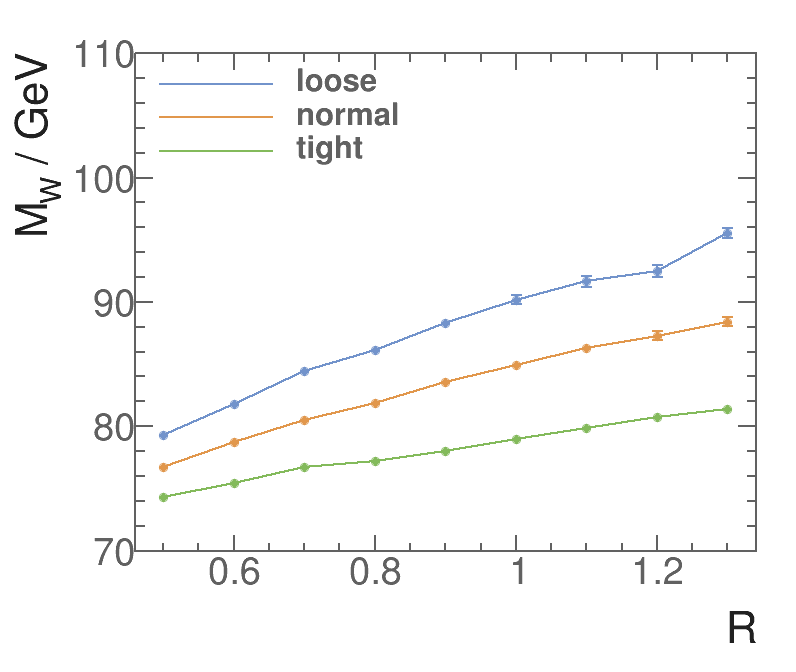
\includegraphics[width=\textwidth]{{doubleHiggs/resolution/ILD_1.4TeV_W_M_testR}.pdf}
    \caption{}
    \label{fig:doubleHiggs1.4WM}
  \end{subfigure}
  \begin{subfigure}[b]{0.45\textwidth}
    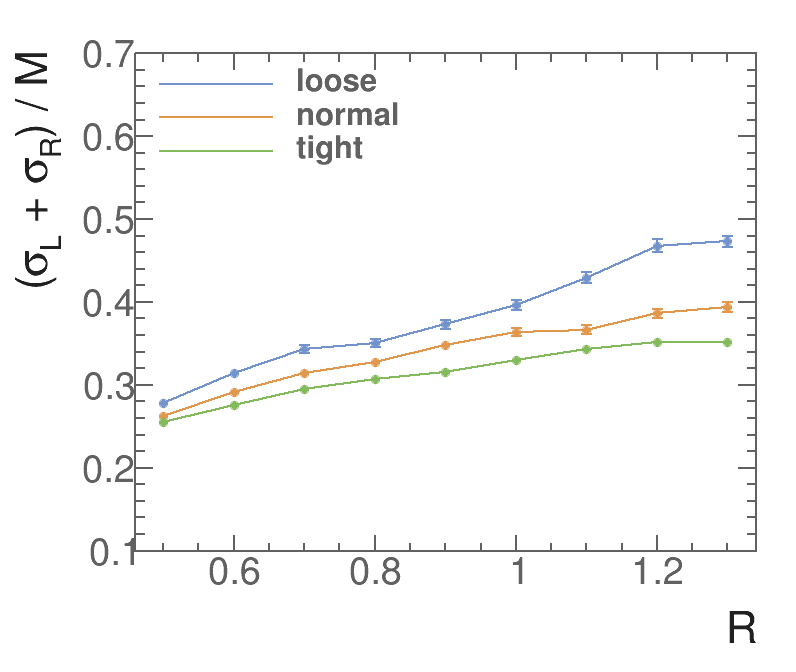
\includegraphics[width=\textwidth]{{doubleHiggs/resolution/ILD_1.4TeV_W_SigmaL_add_SigmaR_divide_M_testR}.pdf}
    \caption{}
    \label{fig:doubleHiggs1.4WSigma}
  \end{subfigure}
\caption[Fitted mass, and resolution of \Hbb, \HWW and \PW at \rootS{1.4}]%
   {Distributions of a) fitted mass peak positions of \Hbb, b) relative mass peak width of \Hbb, c) fitted mass peak positions of \HWW, and f) relative mass peak width of \HWW, e) fitted mass peak positions of \PW, b) relative mass peak width of \PW. All plots show the variation of the fitted masses and mass resolutions as a function of $R$ for  loose, normal and tight selected \PFO collections at \rootS{1.4}.}
   \label{fig:doubleHiggs1.4TeVMassFit}
\end{figure}

\begin{table}[!htbp]
\begin{tabular}{lrr}
\hline
\hline
Fitted jet parameters  &  \rootS{1.4}   &  \rootS{3}  \\
\hline
$\mu_{\Hbb}$ & $122.3_{\pm0.2}$  & $119.1_{\pm0.3}$  \\
$\sigma_{L,\Hbb}$ & $15.2_{\pm0.2}$  & $15.0_{\pm0.3}$  \\
$\sigma_{R,\Hbb}$ & $7.55_{\pm0.16}$ & $8.4_{\pm0.2}$  \\
\hline
$\mu_{\HWW}$ & $125.7_{\pm0.2}$  & $123.0_{\pm0.3}$  \\
$\sigma_{L,\HWW}$ & $29.4_{\pm0.3}$  & $36.6_{\pm0.6}$  \\
$\sigma_{R,\HWW}$ & $7.18_{\pm0.17}$ & $7.4_{\pm0.2}$  \\
\hline
$\mu_{\PW}$ & $80.5_{\pm0.2}$ & $78.1_{\pm0.3}$ \\
$\sigma_{L,\PW}$ & $16.2_{\pm0.3}$ & $13.1_{\pm0.4}$  \\
$\sigma_{R,\PW}$ & $9.03_{\pm0.16}$  &  $9.5_{\pm0.2}$  \\
\hline
\hline
\end{tabular}
\caption
[The fitted mass parameters of optimal jet reconstruction at \rootS{1.4}] %
{The fitted mass  parameters for  \rootS{1.4}  analysis: $R = 0.7$ using the \normalPFO, and for  \rootS{3} analysis: $R = 0.7$ using the \tightPFO.}
\label{tab:doubleHiggsFitParameters}
\end{table}

For the jet reconstruction optimisation at \rootS{3},  \FIGURE{fig:doubleHiggs3TeVMassFit} shows the variation of fitted mass peak positions and  the relative mass resolutions for \Hbb, \HWW, and \PW as function of $R$ and \PFO collections. The relative mass resolution of \PW worsen quickly with increasing $R$. The fitted mass peak positions also increases quicker with the increase of $R$, compared with the fitted positions at \rootS{3}. This is due to at higher centre-of-mass, more beam induced background particles are produced. The background particles, if included in the jets, will increase the invariant masses of the fitted physical bosons. There,  $R = 0.7$  with the \tightPFO is chosen for the \rootS{3} analysis. With chosen parameters, the excellent mass resolutions compensate for the invariant masses slightly smaller than simulated values. The extracted fitted parameters of optimal jet reconstructions at \rootS{3} are summarised in \Table{tab:doubleHiggsFitParameters}.


%This choice  gives good fitted mass peak positions for \Hbb, \HWW and \PW. The extracted fitted parameters of optimal jet reconstructions are summarised in \Table{tab:doubleHiggsFitParameters}.
%The relative mass resolution of \PW worsen with increasing $R$, hence optimal choice favours a small $R$ and \tightPFO. The optimal jet reconstruction parameters is  \tightPFO with $R = 0.7$. The excellent mass resolution with the optimal choice compensates for the invariant masses being slightly smaller than simulated values. The fitted mass peak positions and mass resolutions  1of the chosen jet reconstruction are listed in \Table{tab:doubleHiggs3TeVFitParameters}


\begin{figure}[!tbp]
  \begin{subfigure}[b]{0.45\textwidth}
    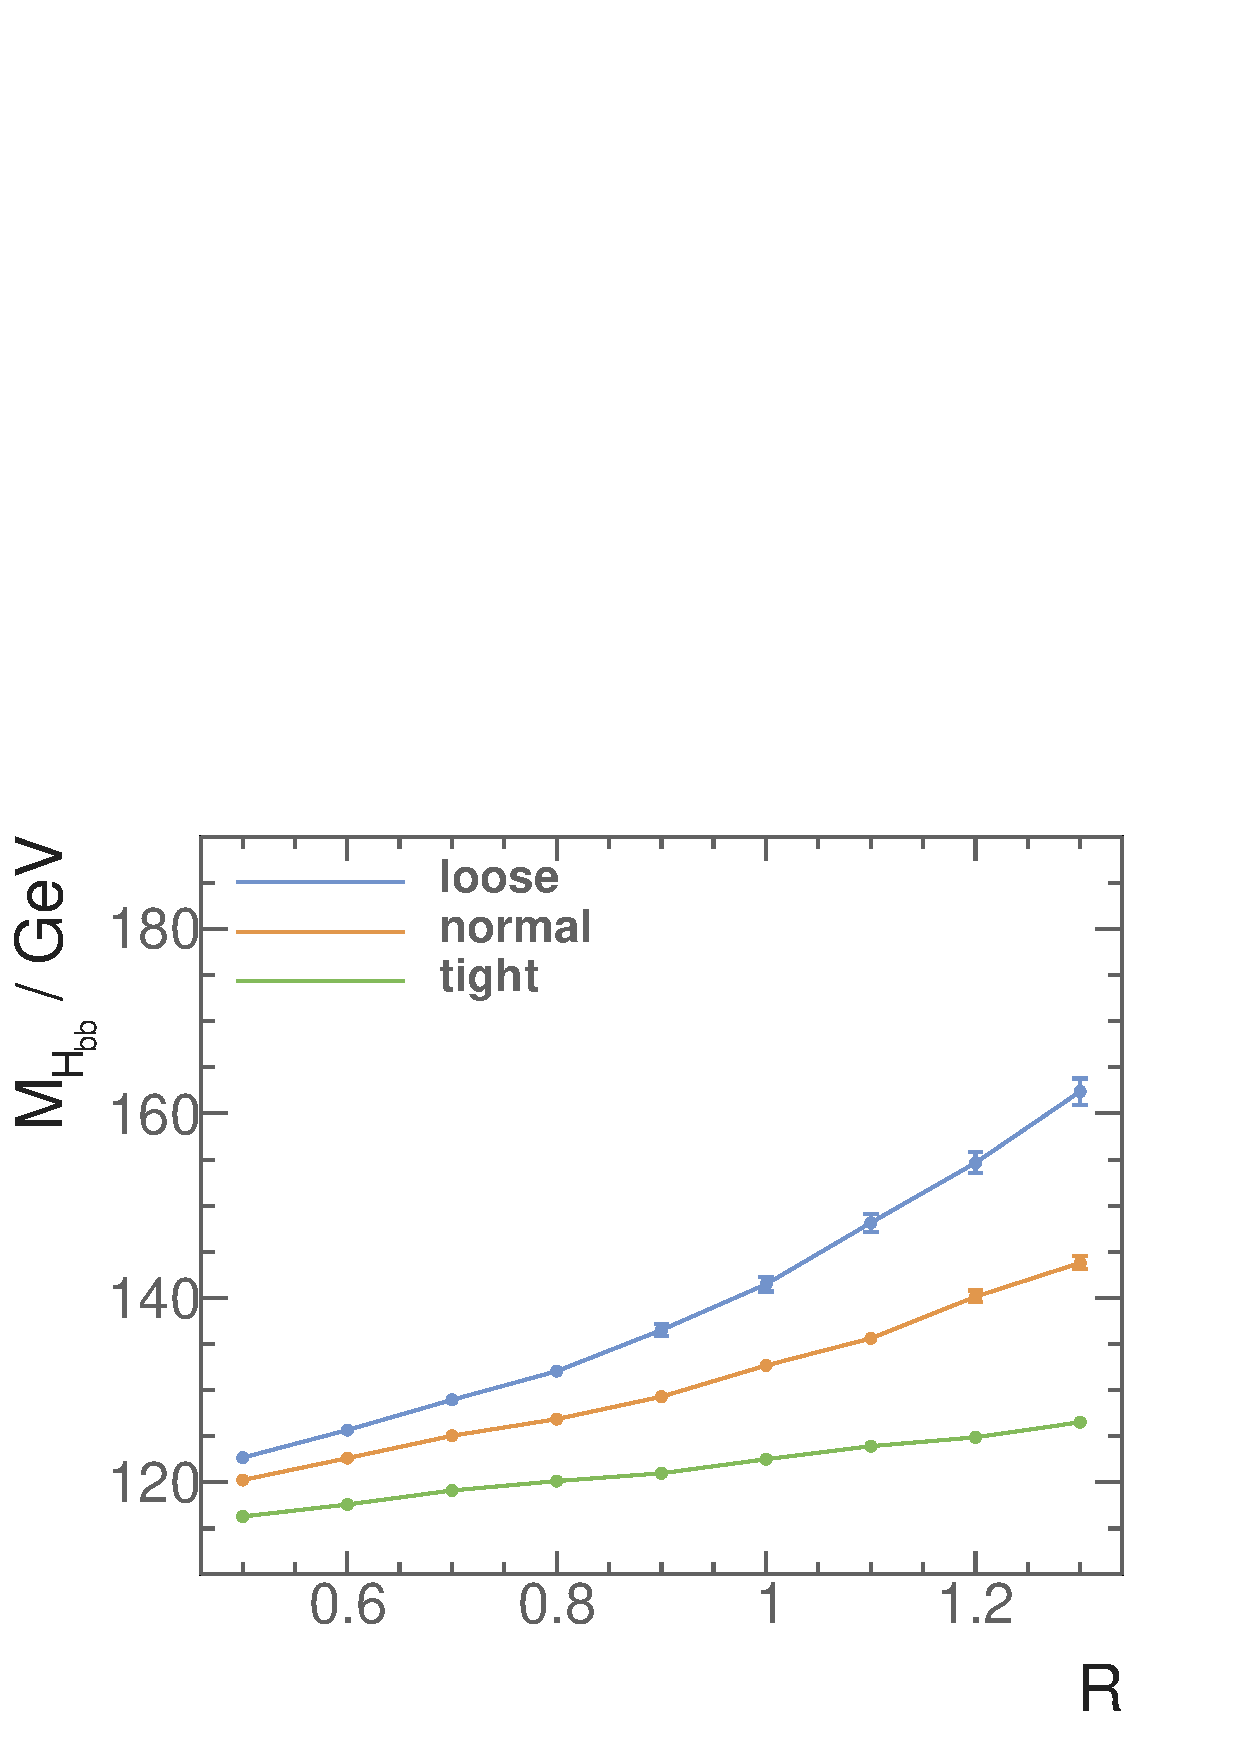
\includegraphics[width=\textwidth]{{doubleHiggs/resolution/ILD_3TeV_Higgs1_M_R}.pdf}
    \caption{}
    \label{fig:doubleHiggs3Higgs1M}
  \end{subfigure}
  \begin{subfigure}[b]{0.45\textwidth}
    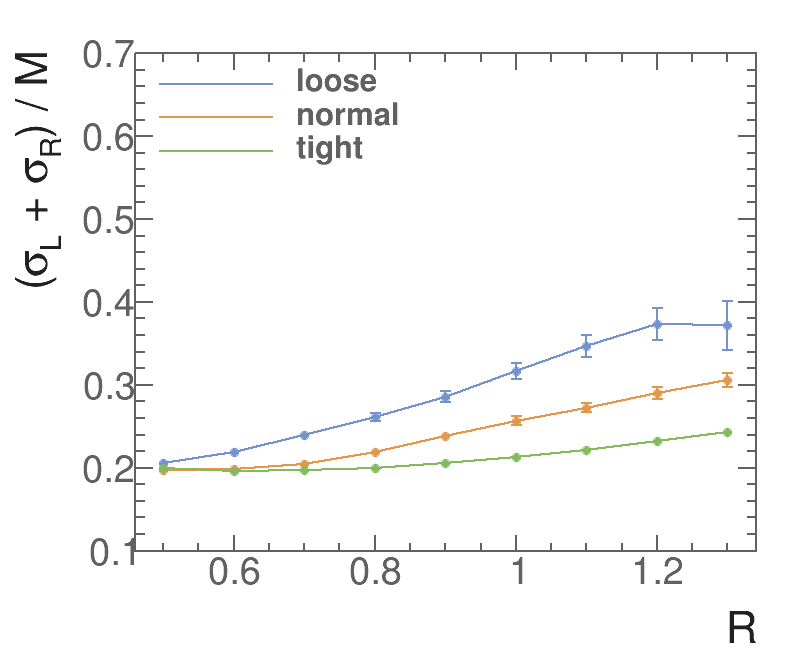
\includegraphics[width=\textwidth]{{doubleHiggs/resolution/ILD_3TeV_Higgs1_SigmaL_add_SigmaR_divide_M_testR}.pdf}
    \caption{}
    \label{fig:doubleHiggs3Higgs1Sigma}
  \end{subfigure}
  \begin{subfigure}[b]{0.45\textwidth}
    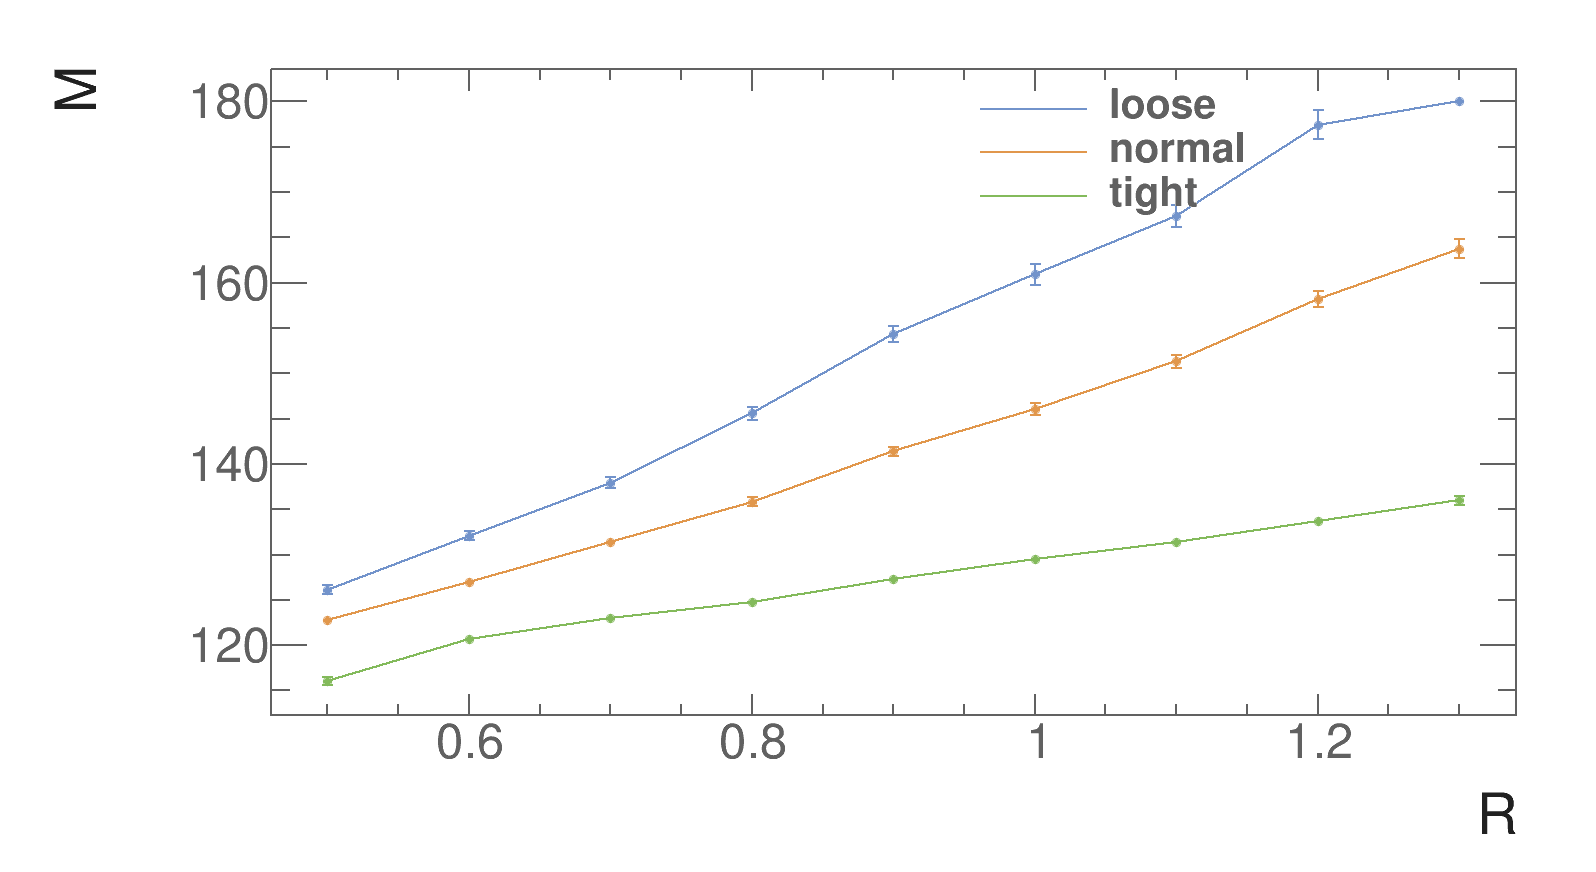
\includegraphics[width=\textwidth]{{doubleHiggs/resolution/ILD_3TeV_Higgs2_M_R}.pdf}
    \caption{}
    \label{fig:doubleHiggs3Higgs2M}
  \end{subfigure}
  \begin{subfigure}[b]{0.45\textwidth}
    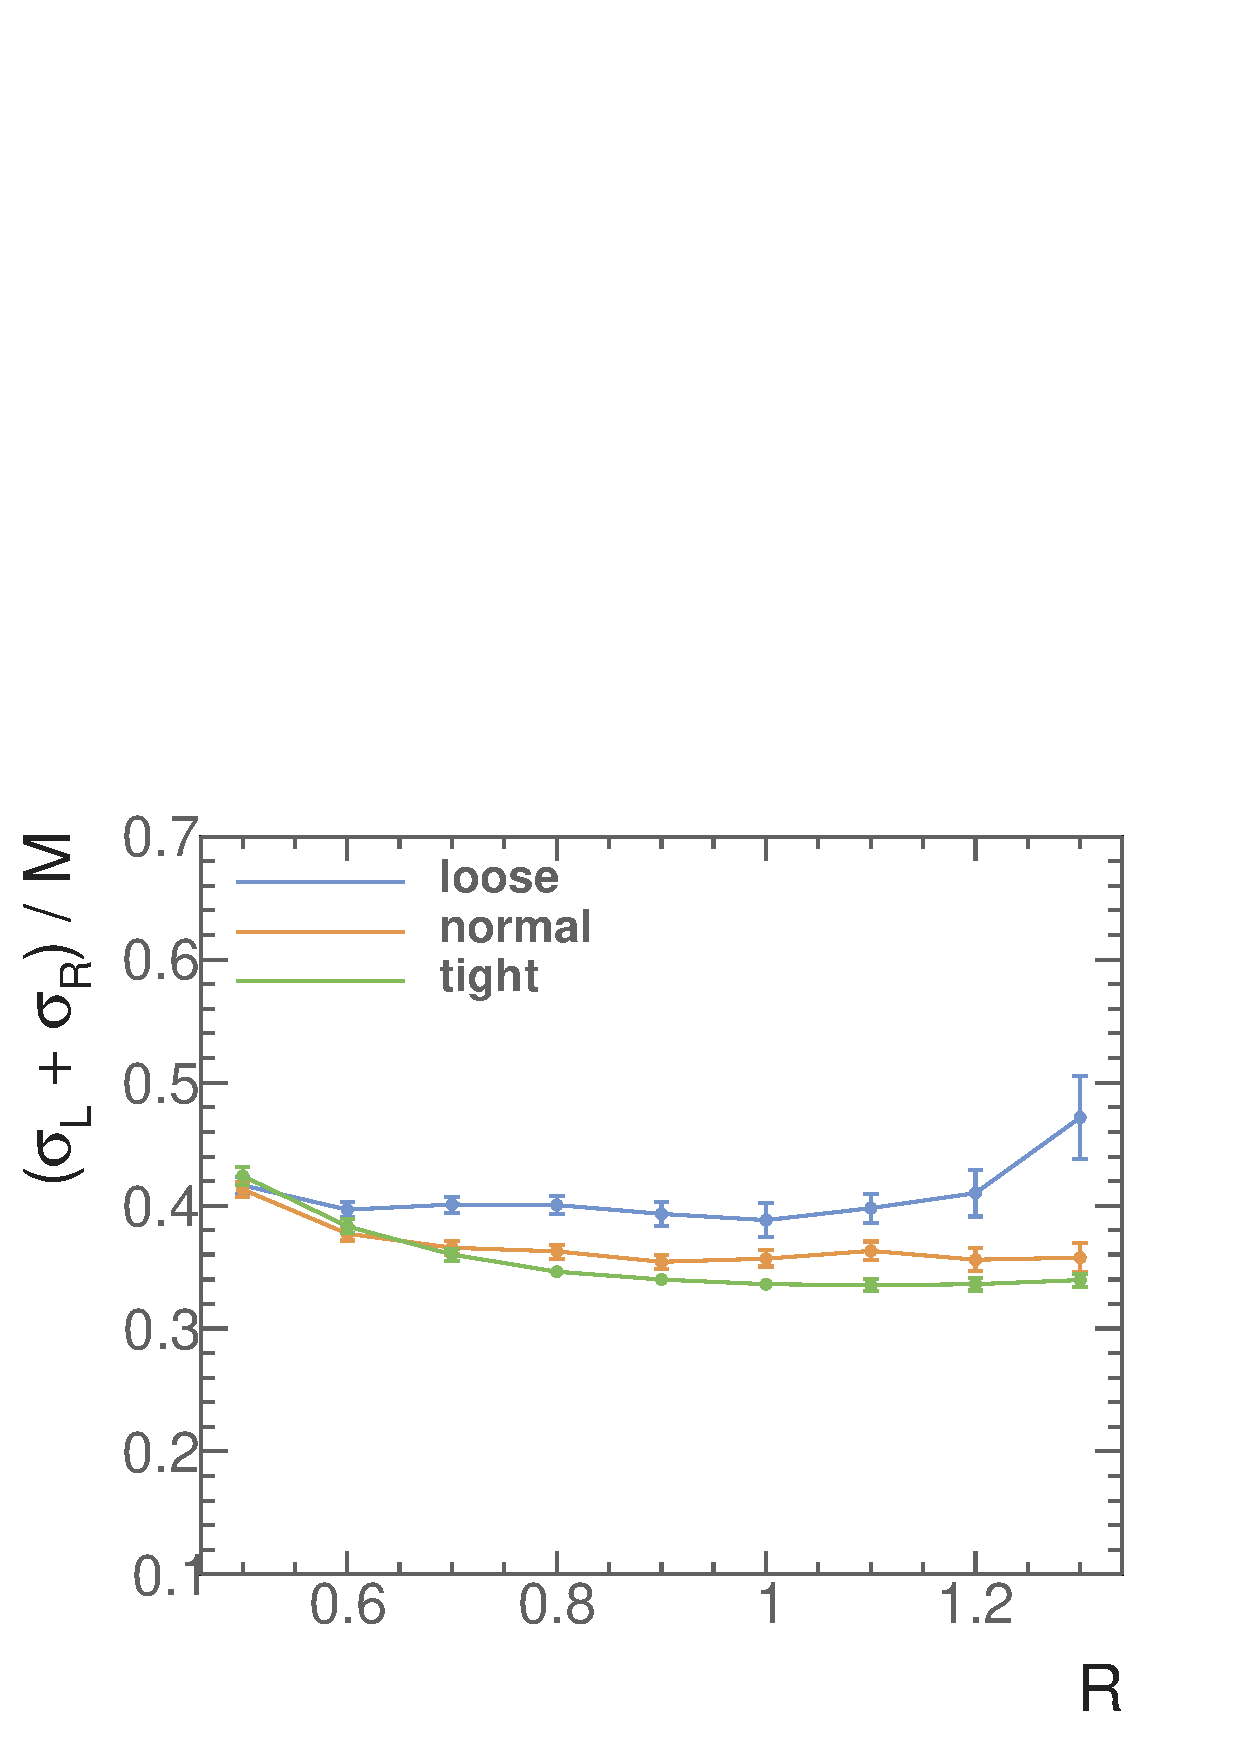
\includegraphics[width=\textwidth]{{doubleHiggs/resolution/ILD_3TeV_Higgs2_SigmaL_add_SigmaR_divide_M_testR}.pdf}
    \caption{}
    \label{fig:doubleHiggs3Higgs2Sigma}
  \end{subfigure}
  \begin{subfigure}[b]{0.45\textwidth}
    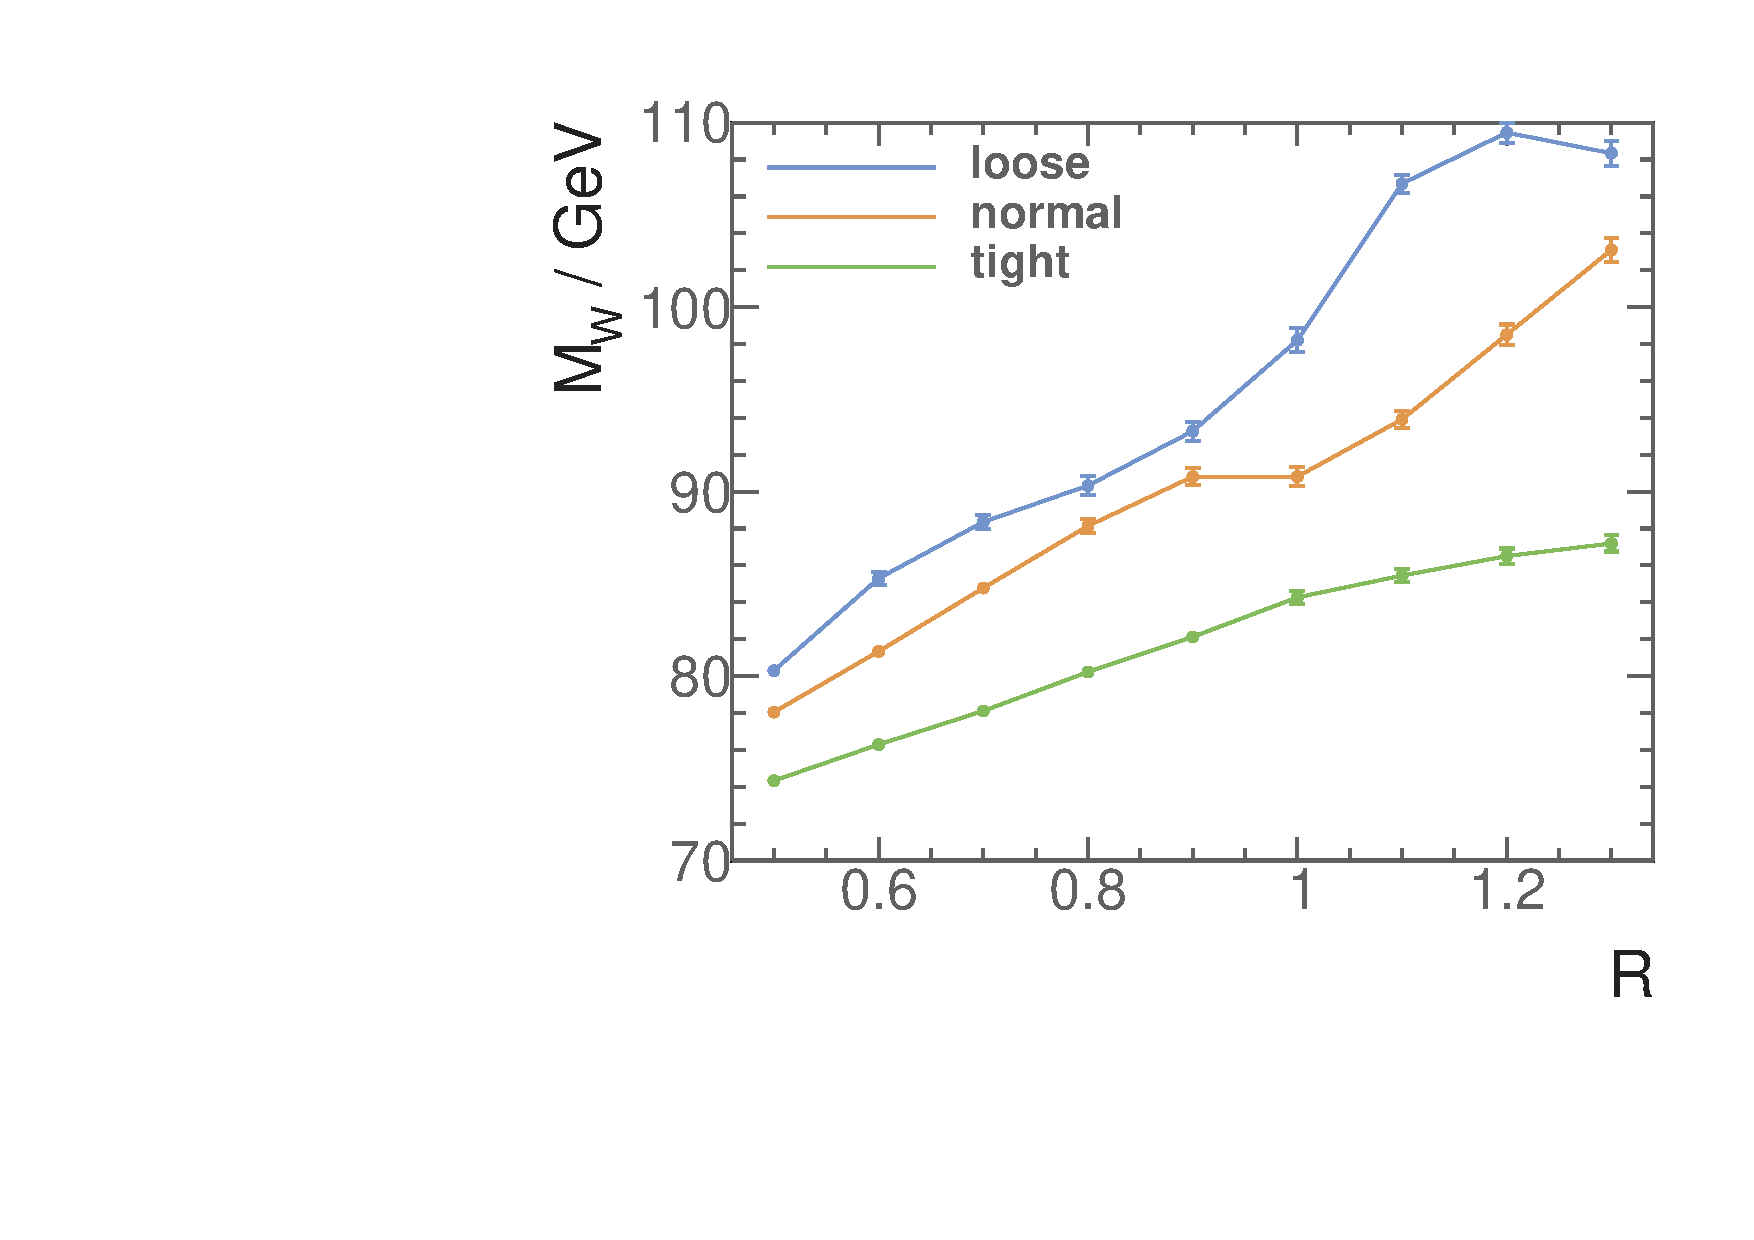
\includegraphics[width=\textwidth]{{doubleHiggs/resolution/ILD_3TeV_W_M_testR}.pdf}
    \caption{}
    \label{fig:doubleHiggs3WM}
  \end{subfigure}
  \begin{subfigure}[b]{0.45\textwidth}
    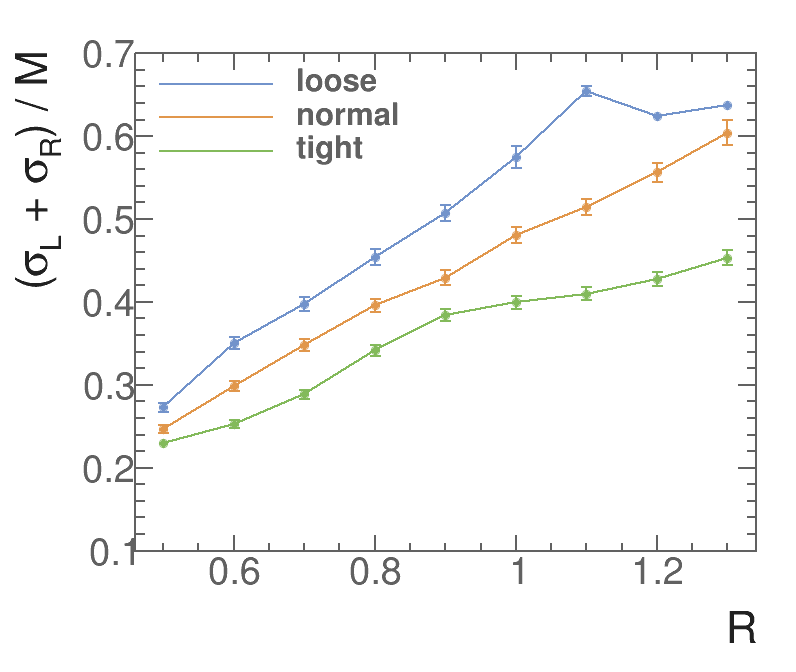
\includegraphics[width=\textwidth]{{doubleHiggs/resolution/ILD_3TeV_W_SigmaL_add_SigmaR_divide_M_testR}.pdf}
    \caption{}
    \label{fig:doubleHiggs3WSigma}
  \end{subfigure}
\caption[Fitted mass peak positions and relative mass resolution of \Hbb, \HWW and \PW at \rootS{3}.]%
{Distributions of a) fitted mass peak positions of \Hbb, b) relative mass peak width of \Hbb, c) fitted mass peak positions of \HWW, d) relative mass peak width of \HWW, e) fitted mass peak positions of \PW, and f) relative mass peak width of \PW. All plots show the variation of fitted masses and mass resolutions as a function of $R$ for  loose, normal and tight selected \PFO collections at \rootS{3}.}
   \label{fig:doubleHiggs3TeVMassFit}
\end{figure}

\section{Jet flavour tagging}
\label{sec:doubleHiggsFlavourTagging}

As the signal channel, \eeToHHbbWWHad,  has two \Pbottom quarks in the final state, identifying jets originated from \Pbottom quarks is an important part of the event selection. To establish the likelihood of a \Pbottom jet (b-jet tag value), \lcfiplus \cite{Suehara:2015ura} software package is used.

%Another useful analysis technique is to identify jets from \Pbottom and \Pcharm quarks. These jets have signatory topologies. A combination of vertex finding and multivariate analysis is used to identify \Pbottom and \Pcharm jets.

The flavour tagging processor, \lcfiplus \cite{Suehara:2015ura} is based on the LCFIVertex package \cite{Bailey:2009ui}, which was used in the simulation studies for the \ILCloi \cite{Abe:2010aa,Aihara:2009ad} and the \CLICcdr \cite{Linssen:2012hp}.  \lcfiplus is modular and can be used in any order. However here it will be described in the order that is used in this analysis.

%The current software is built for a future \ee collider.

The inputs are \PFOs, after jet clustering using $R = 0.7$ and the \normalPFO. The vertex finding algorithms in the \lcfiplus perform vertex fitting and identify primary and secondary vertices. There is a ``V0'' particle rejection step.  A ``V0'' particle is a  neutral particle that decays into pairs of charged particles. The topology of the ``V0'' particles can be  similar to the decay of \Pbottom or \Pcharm quarks. Hence it is important to remove the ``V0' particles to improve the b-quark and c-quark flavour tagging (see \Section{sec:pandoraPandoraTrack} for a similar V0 rejection).

Once the primary and secondary vertices are found, \PFOs are re-clustered into jets. This jet re-clustering scheme ensures that the secondary vertices and the muons which is identified from semi-leptonic decay of the quarks, fall into the same jet. Therefore, the topology of the jet is consistent with the  hadronic decay of heavy quarks. The jet re-clustering scheme are Durham and Durham modified algorithms (see \Section{sec:pandoraJetDurham}).

The next step is to refine vertices to improve the \Pbottom jet severation from the \Pcharm jet.  Additional information is applied to improve the vertex reconstruction. Since the existence of two close by vertices is strongly correlated to a \Pbottom jet, the vertices refining step will reconstruct as many secondary vertices correctly as possible.

The last step is to gather the information about vertices and jets, and deploy a multivariate analysis. The multivariate classier used, Boosted Decision Tree,  is implemented in the TMVA software package \cite{Hocker:2007ht}. A number of flavour sensitive variables are calculated. The jets are is divided into four subsets: jets with zero, one, two properly reconstructed vertices, or a single-track pseudo-vertex. For each subset, a jet can either be classified to a \Pbottom jet, a \Pcharm jet, or a light flavour quark jet (\Pup, \Pdown or \Pstrange). The multiclass classifier's response is normalised across different subsets.
%, and they will be referred in the subsequent physics analysis as the tag value.

%The samples for training the multiclass classifier are \HepProcess{\Pep \Pem \to \PZ \APnu \Pnu} at \rootS{1.4}, where \PZ decays to \HepProcess{\Pbottom\APbottom}, \HepProcess{\Pcharm\APcharm}, or \HepProcess{\Pup\APup/\Pdown\APdown/\Pstrange\APstrange}.

The events to train the multiclass classifier are \HepProcess{\Pep \Pem \to \PZ \APnu \Pnu} event at \rootS{1.4}, where \PZ decays to \HepProcess{\Pbottom\APbottom}, \HepProcess{\Pcharm\APcharm}, or \HepProcess{\Pup\APup/\Pdown\APdown/\Pstrange\APstrange}. The selection efficiency of b jets and c jets with the training samples is shown in \Figure{fig:doubleHiggs1.4Btag}. The normalised distribution of the highest b-jet tag value for the signal events is shown in \Figure{fig:doubleHiggsBtagSignalPerformance}.

%To apply trained  multiclass classifier in the \lcfiplus processor, all the \PFOs in the initial reconstructed jet are fed into the processor. The jet re-clustering step in the \lcfiplus is set to find six jets. For each jet, values for the likelihood of a b-jet and a c-jet are obtained.
%At the training stage, the  jet re-clustering step is set to find two jets.  he outputs for a jet is three values, corresponding to the likelihood of the jet being a b-jet, a c-jet, or a light flavour quark jet.


For the \rootS{3}, the flavour tagging processor is re-trained in the same way as in the \rootS{1.4} analysis. The training events are from the same channel but at \rootS{3}. The performance of the flavour tagging  with training samples is shown in \Figure{fig:doubleHiggsBtag3TeV}. Compared to the performance at \rootS{1.4}, the performance is slightly worse, because at high centre-of-mass, particles at more collimated and more difficult to separate. Therefore, the vertex identification and the flavour tagging performance are worse.
%high energy or high energies?

\begin{figure}[!htbp]
 \begin{subfigure}[b]{0.45\textwidth}
    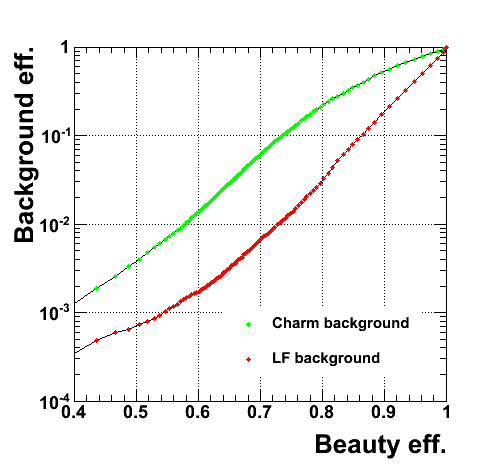
\includegraphics[width=\textwidth]{{doubleHiggs/eval-lcfiweights_R0_7_2jets-test}.pdf}
    \caption{\rootS{1.4}}
    \label{fig:doubleHiggsBtag3TeV}
  \end{subfigure}
 \begin{subfigure}[b]{0.45\textwidth}
    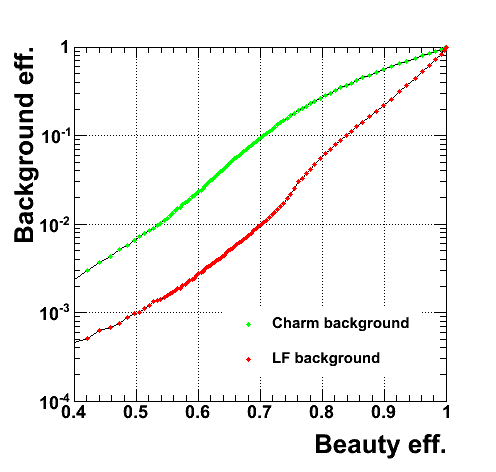
\includegraphics[width=\textwidth]{{doubleHiggs/eval-lcfiweights_tR0_7_3000_2jets-test}.pdf}
    \caption{\rootS{3}}
   \label{fig:doubleHiggs1.4Btag}
  \end{subfigure}
\caption
   {Performance of b-jet tagging with training samples at a) \rootS{1.4}, b) \rootS{3}.}
   \label{fig:doubleHiggsBtag}
\end{figure}


\begin{figure}[!htbp]
    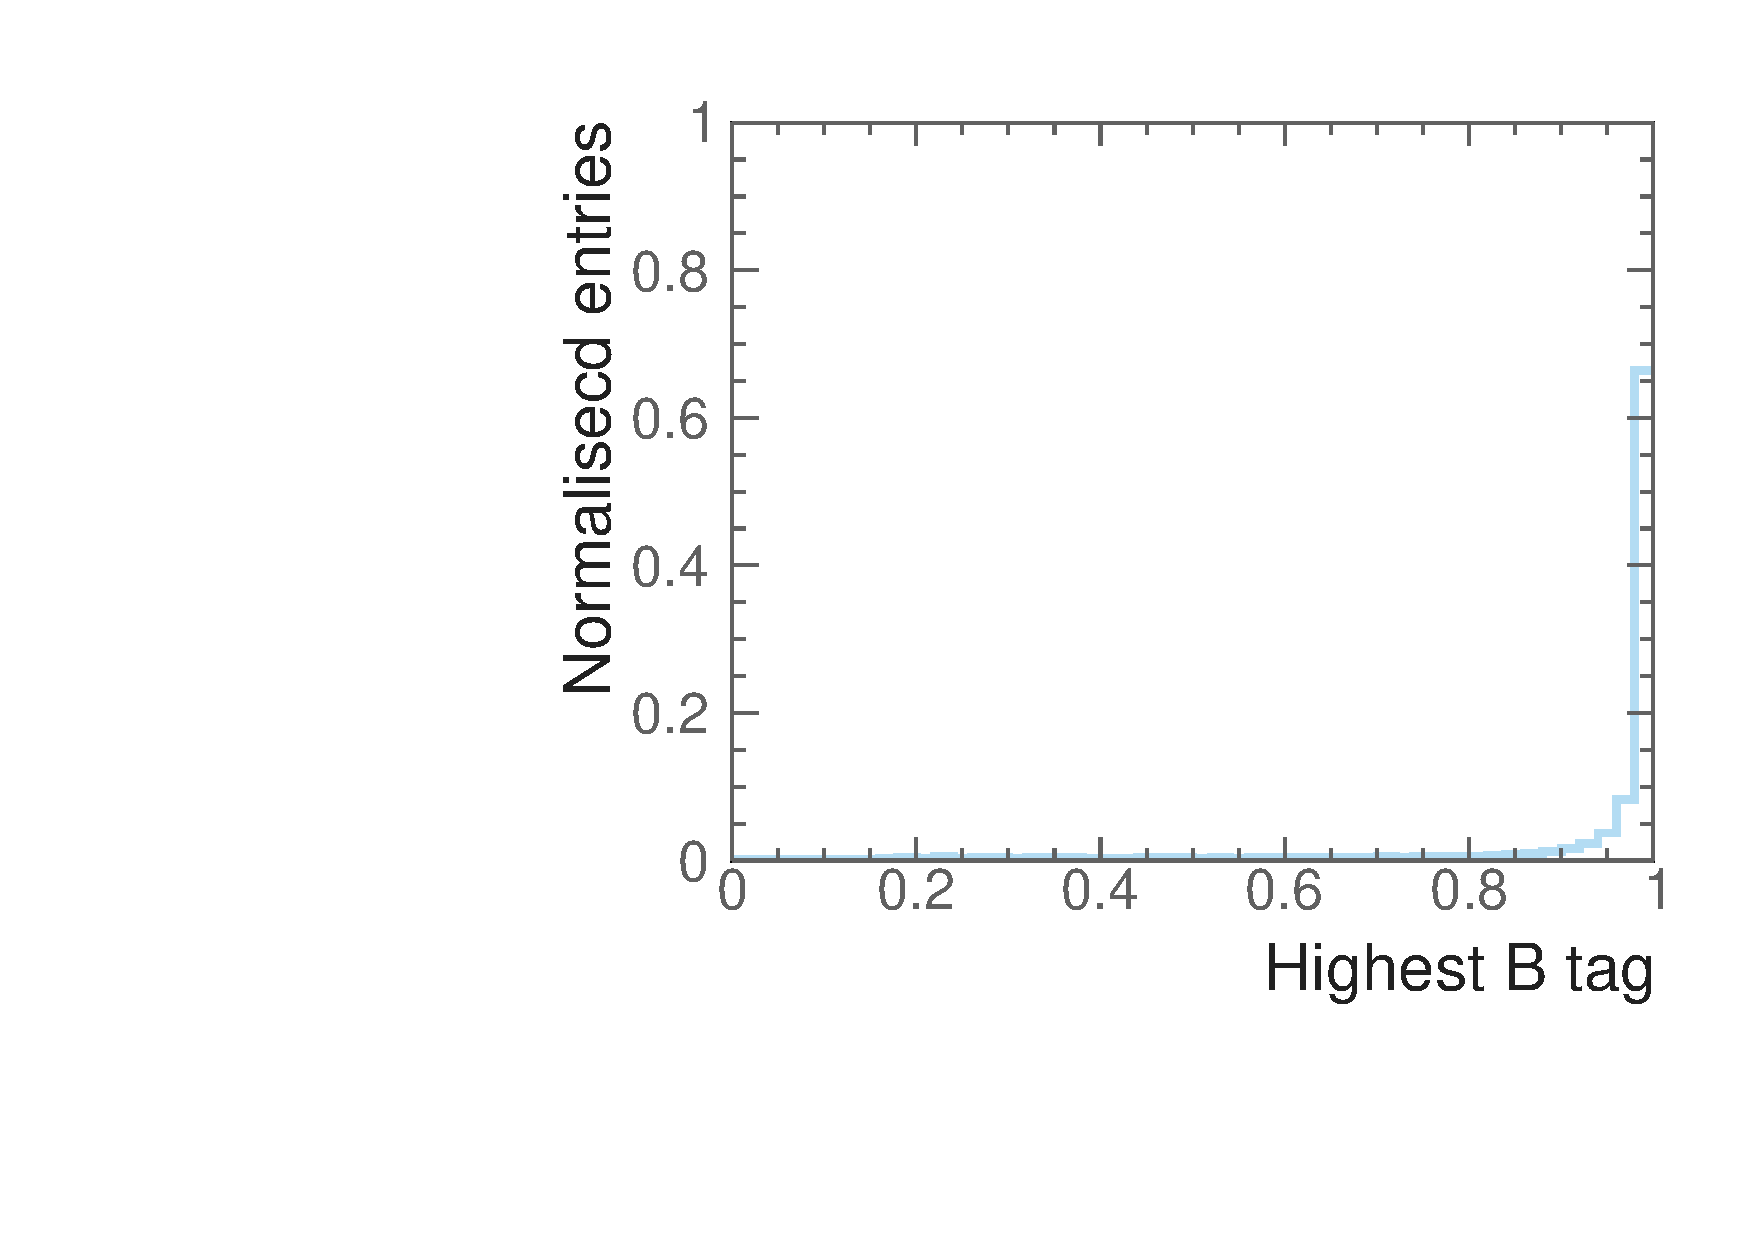
\includegraphics[width=0.45\textwidth]{{doubleHiggs/jetPairing/nR0_7_6jet_btag2_bTag1_TMVA20170223R0_7_qq_btag2_prepare}.pdf}
\caption
   {The normalised distribution of the highest b-jet tag value for the signal events  at \rootS{1.4}}
   \label{fig:doubleHiggsBtagSignalPerformance}
\end{figure}
%The flavour tagging is performed after the initial jet reconstruction, and all the \PFOs in the reconstructed jets are input into the \lcfiplus flavour tagging processor. Therefore, the classifier in the \lcfiplus processor is trained for a specific \PFO collection and a specific jet reconstruction algorithm. The outputs of the processor for a jet are three values, corresponding to the likelihood of the jet being a \Pbottom jet, a \Pcharm jet, or a light flavour quark jet.

%The flavour tagging is performed after the initial jet reconstruction using optimal jet reconstruction parameters.  \PFOs in the reconstructed jets are the inputs to the flavour tagging processor. \lcfiplus processor includes a multiclass classifier which needs to be trained.


\subsection{Mutually exclusive cuts for \eeToHHbbWW and \eeToHHbbbb}
\label{sec:doubleHiggsMutualExclusive}

Two \eeToHH final states with largest branching fractions are \eeToHHbbbb (31.5\%) and \eeToHHbbWW (25.9\%). Two final states have different topologies and are subject of two analysis strategies. The \eeToHHbbWW final state is the subject of this thesis.  The study of the \eeToHHbbbb final state is the subject of an independent analysis. A set of cuts are designed to separate  samples, for both signal and background events, into two mutually exclusive sets for  two independent analyses. This ensures there are no correlations between two analyses.

%This eases the difficulty of combining sub-channels as correlations between sub-channels need not to be considered where samples are mutually exclusive.
%With the jet clustering and b-jet tagging information,

The most distinctive difference between the two sub-channels is the different number of jets and the different number of b-jets in the final state. Variables relating to the number of b-jets and number of overall jets are suitable for separating two sub-channels.

 \FIGURE{fig:doubleHiggsMutualPreselection} shows the sum of b-jet tag values, when the event is clustered into four jets, as a function of $-\log\parenths{\y{34}}$ for the hadronic \WW decay in \eeToHHbbWW and \eeToHHbbbb. \y{} parameter is a measure of number of jets. As expected,  two sub-channels can be clearly separated in this two dimensional phase space. A rectangular cut will separate the phase space into two spaces, donated as $S$ and $\neg{S}$. The hadronic \WW decay in \eeToHHbbWW events should  be contained in  $S$, and the \eeToHHbbbb events should be contained in $\neg{S}$.

To maximise the separation of two sub-channels, a set of cuts are found by maximising the product of the fraction of the sub-channel events in each space:
\begin{equation}
\varepsilon = \frac{N_{\text{\eeToHHbbWW, hadronic}} \in S} {N_{\text{\eeToHHbbWW, hadronic}}} \times \frac{N_{\eeToHHbbbb} \in \neg{S}} {N_{\eeToHHbbbb}} ,
\end{equation}
where $N \in S$ indicates number of events in the phase space $S$.

Several variables are tested to maximise $\varepsilon$. The best cuts found defining $S$ is $\sumBtag{4} < 2.3, \,-\log\parenths{\y{34}} < 3.7$. With the cuts, 86\% of  the hadronic \WW decay in \eeToHHbbWW events are in $S$ and 78\% of the \eeToHHbbbb events are in $\neg{S}$. The full list of fraction of events after passing mutually exclusive cuts for individual background channel can be found in \Table{tab:doubleHiggs1.4TeVPreslection}.


\begin{figure}[!tbp]
  \begin{subfigure}[b]{0.45\textwidth}
    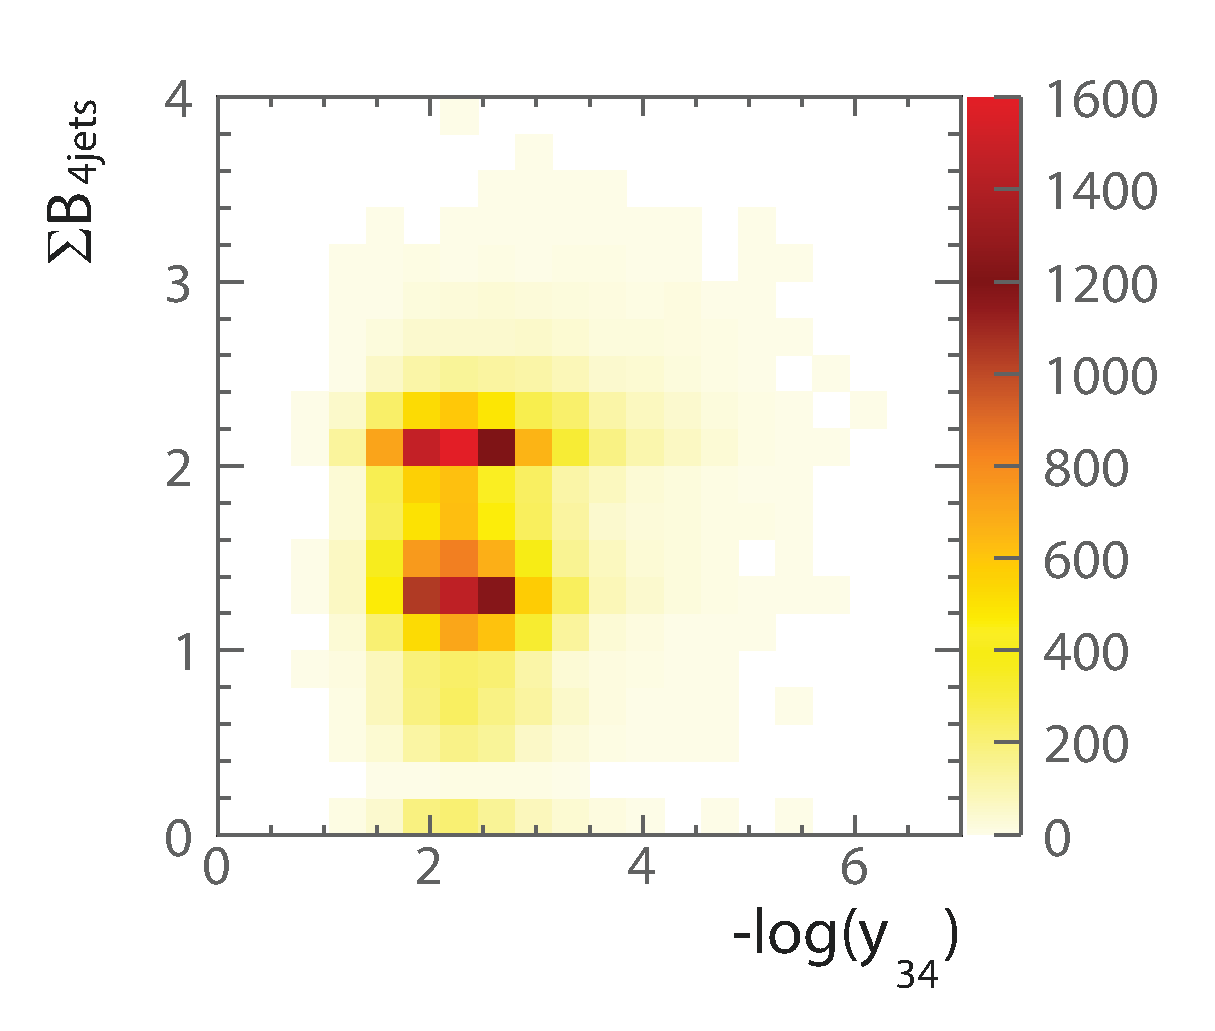
\includegraphics[width=\textwidth]{doubleHiggs/preSel/mutual6022bbWW2}
    \caption{\eeToHHbbWW, hadronic}
    \label{fig:doubleHiggs1.4MutualbbWW}
  \end{subfigure}
    \begin{subfigure}[b]{0.45\textwidth}
    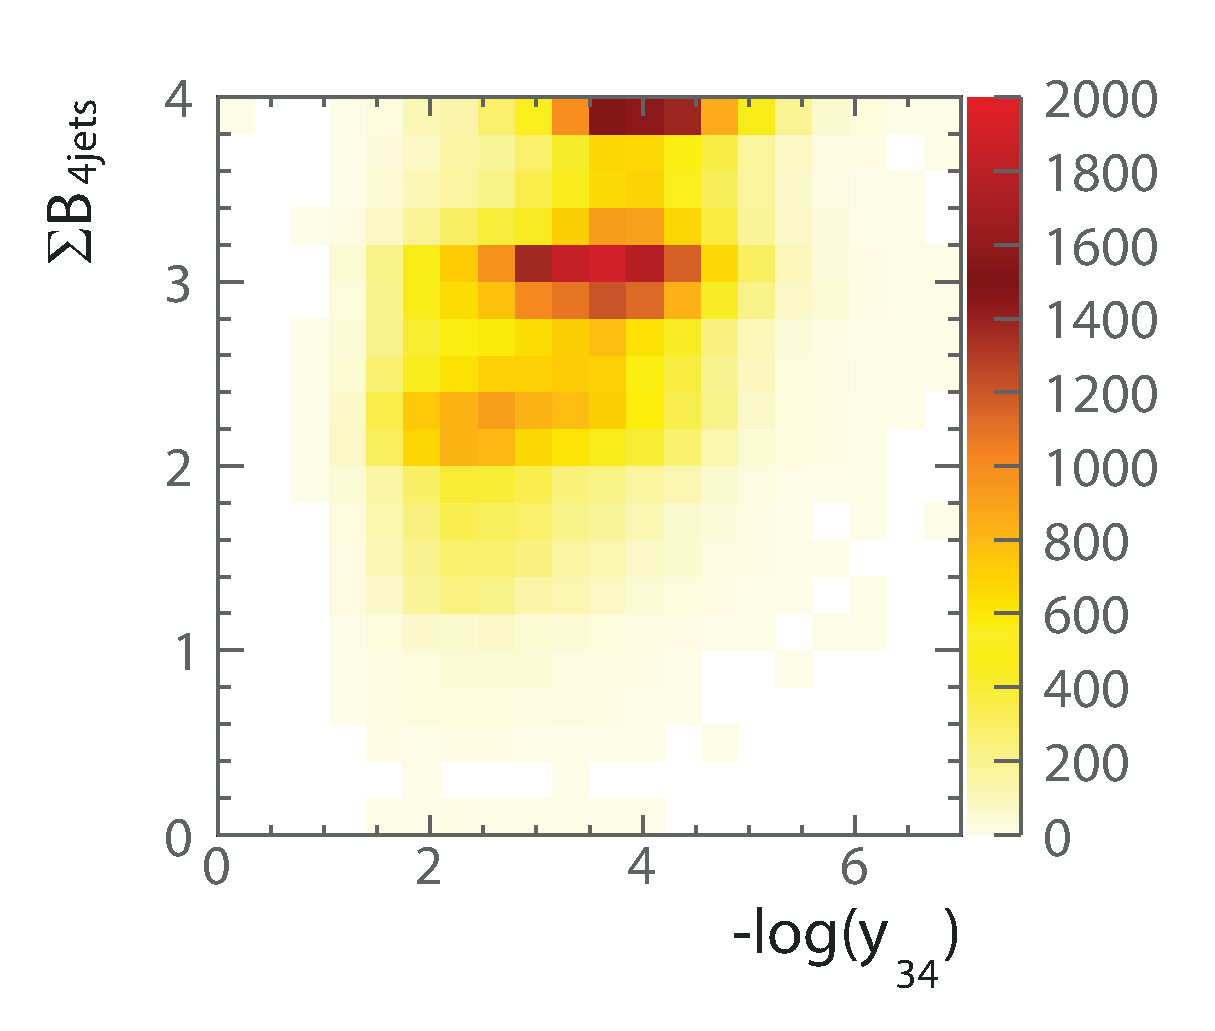
\includegraphics[width=\textwidth]{doubleHiggs/preSel/mutual6022bbbb2}
    \caption{\eeToHHbbbb}
    \label{fig:doubleHiggs1.4Mutualbbbb}
  \end{subfigure}
\caption[Sum of b-jet tag values as a function of $-\log\parenths{\y{34}}$ at \rootS{1.4}]%
   {Sum of b-jet tag values, when the event is clustered into four jets, as a function of $-\log\parenths{\y{34}}$ at \rootS{1.4}, shown for hadronic \WW decay of \eeToHHbbWW and \eeToHHbbbb sub-channel. }
   \label{fig:doubleHiggsMutualPreselection}
\end{figure}


\section{Jet pairing}

Having optimised the jet reconstruction, and obtained the six jets from the jet re-clustering step in the \lcfiplus processor, the next step is to group jets according to signal event topology.
Jets are paired up such that there are two jets for \HepProcess{\PHiggs \to \Pbottom \APbottom}, two jets for hadronic decay of a \PW, two jets  for hadronic decay  of a \W*, and the two $\PW{s}$ forming a  \PHiggs boson.

Six jets are associated to \Hbb, \PW and \W*. There are 90 possible permutations. The best permutation is obtained by minimising a $\chi^2$  based on expected masses and mass widthes:

%off-mass-shell and off the mass shell? Is the "the" pertinent? Should they both be hyphenated?

%The jet pairing scheme provides reconstructed invariant masses of \Hbb, \HWW, and \PW. The jet pairing metric states:
\begin{equation}
	\chi^2 = \left(\frac{m_{ij}-\mu_{\Hbb}}{\sigma_{\Hbb}^{\prime}}\right)^2 + \left(\frac{m_{klmn}-\mu_{\HWW}}{\sigma_{\HWW}^{\prime}}\right)^2  + \left(\frac{m_{kl}-\mu_{\PW}}{\sigma_{\PW}^{\prime}}\right)^2,
%\label{eqn:eq_chi2_HHWWbb}
\end{equation}

\begin{equation}
	\sigma_{\Hbb}^{\prime}=
    \begin{cases}
      \sigma_{L,\Hbb}, & \text{if}\ m_{ij} < \mu_{\Hbb}, \\
     \sigma_{R,\Hbb}, & \text{otherwise}, \\
   \end{cases}
   \,\text{etc.}
\end{equation}

\begin{comment}
\begin{equation}
	\sigma_{\HWW}^{\prime}=
    \begin{cases}
      \sigma_{L,\HWW}, & \text{if}\ m_{klmn} < \mu_{\HWW}\\
     \sigma_{R,\HWW}, & \text{otherwise} \\
   \end{cases}
\end{equation}


\begin{equation}
	\sigma_{\PW}^{\prime}=
    \begin{cases}
      \sigma_{L,\PW}, & \text{if}\ m_{kl} < \mu_{\PW}\\
     \sigma_{R,\PW}, & \text{otherwise} \\
   \end{cases}
\end{equation}
\end{comment}
where the indices $i$ to $l$ indicate the one of the six jets, $\mu$ and $\sigma$ are the fitted invariant mass and the fitted width from \Table{tab:doubleHiggsFitParameters}. The asymmetrical structure of the fitting function is reflected in the jet pairing $\chi^2$. The jet pairing is only considered when at least one of the jets associated to the \Hbb decay with a b-jet tag > 0.2. Of these combinations of jets, the jet pairing giving smallest  $\chi^2$ is selected. The normalised distribution of $m_{\Hbb}$ after jet pairing, for the signal channel, \eeToHHbbWW and the sum of all background channels can be seen in \Figure{fig:doubleHiggsJetPairing}. For the signal channel, the distribution peaks around the expected mass of $m_{\Hbb}$. It can also be seen from the figures that around 1\% of the signal events have no solutions for the jet pairing, as no jet has a b-jet tag > 0.2. The full list of fraction of events after jet pairing selection can be found in \Table{tab:doubleHiggs1.4TeVPreslection}.


\begin{figure}[!htbp]
 \begin{subfigure}[b]{0.45\textwidth}
    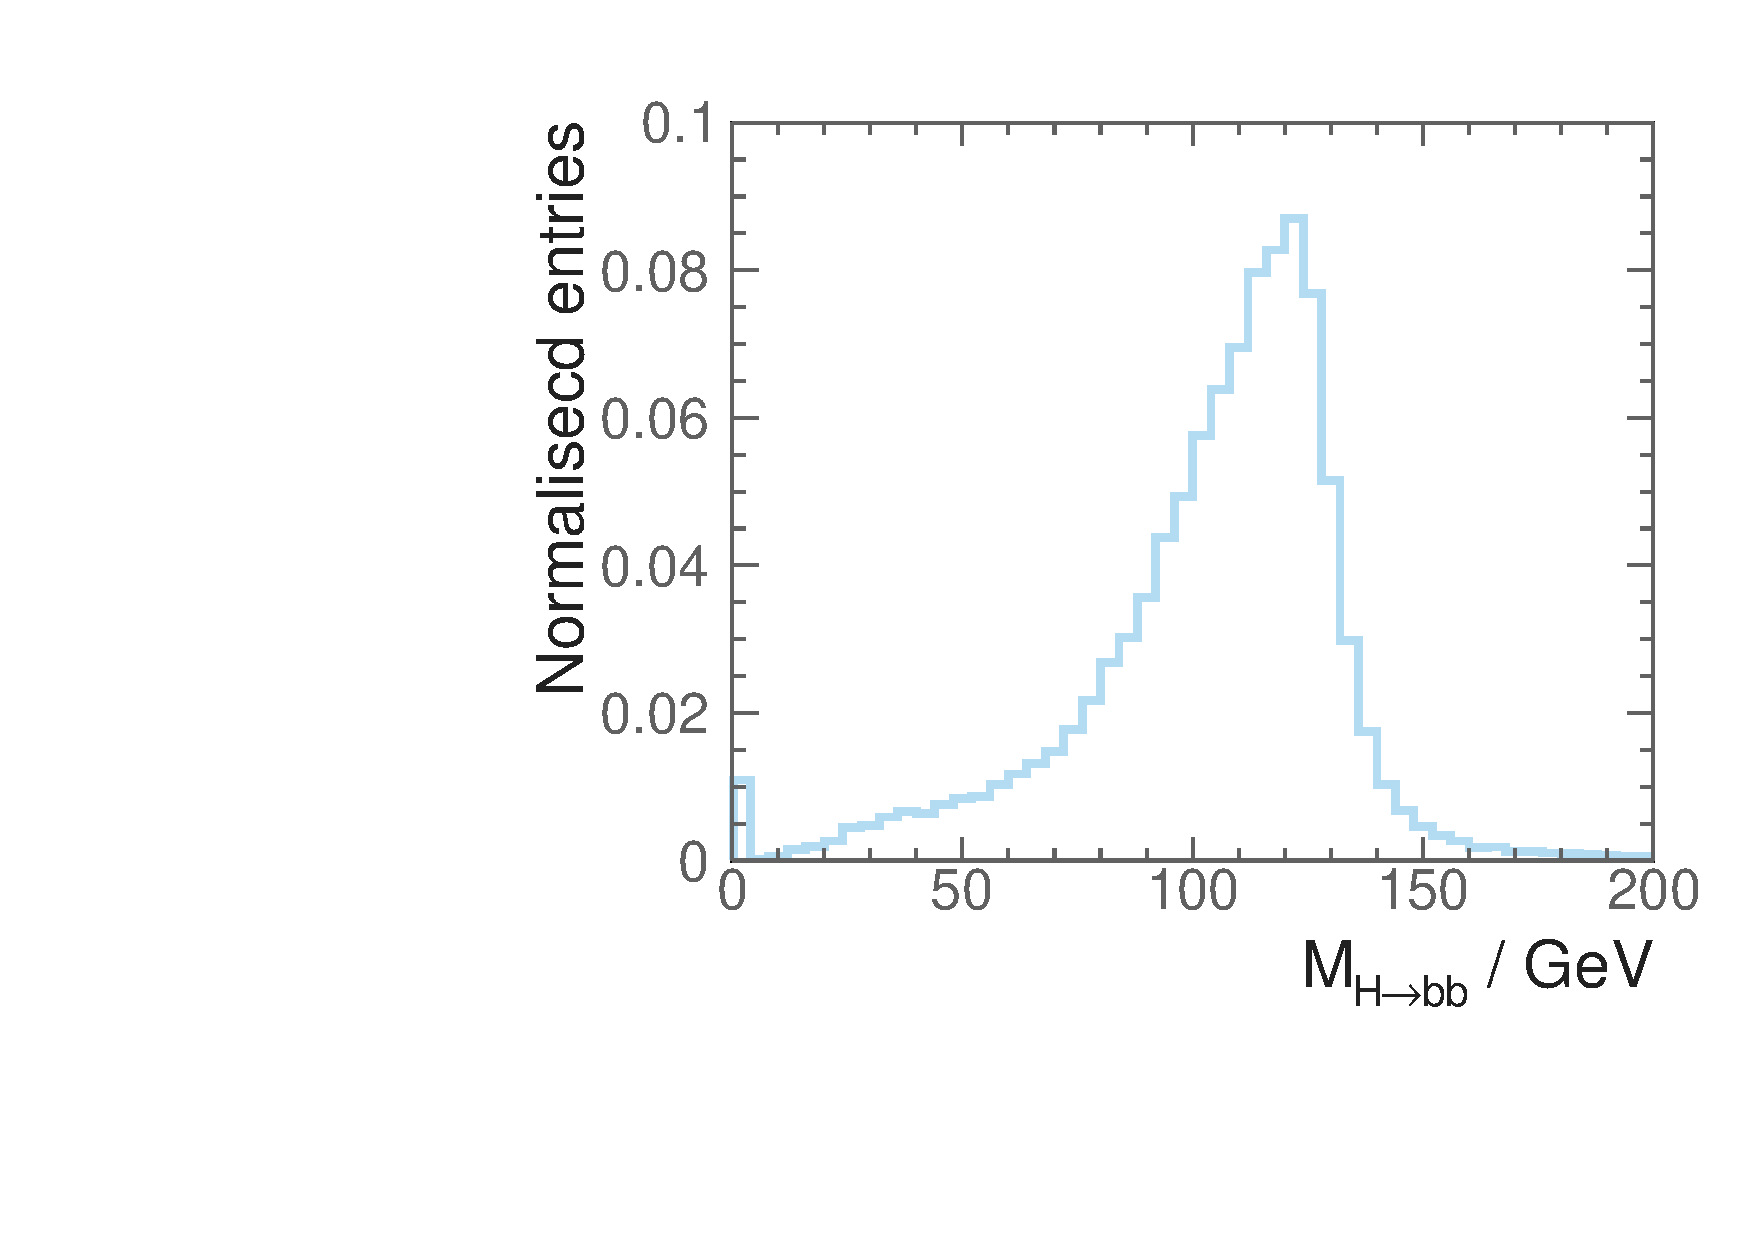
\includegraphics[width=\textwidth]{{doubleHiggs/jetPairing/nR0_7_6jet_btag2_Higgs1_M_TMVA20170223R0_7_qq_btag2_prepare}.pdf}
    \caption{Signal}
    \label{fig:doubleHiggsJetPairingSignal}
  \end{subfigure}
 \begin{subfigure}[b]{0.45\textwidth}
    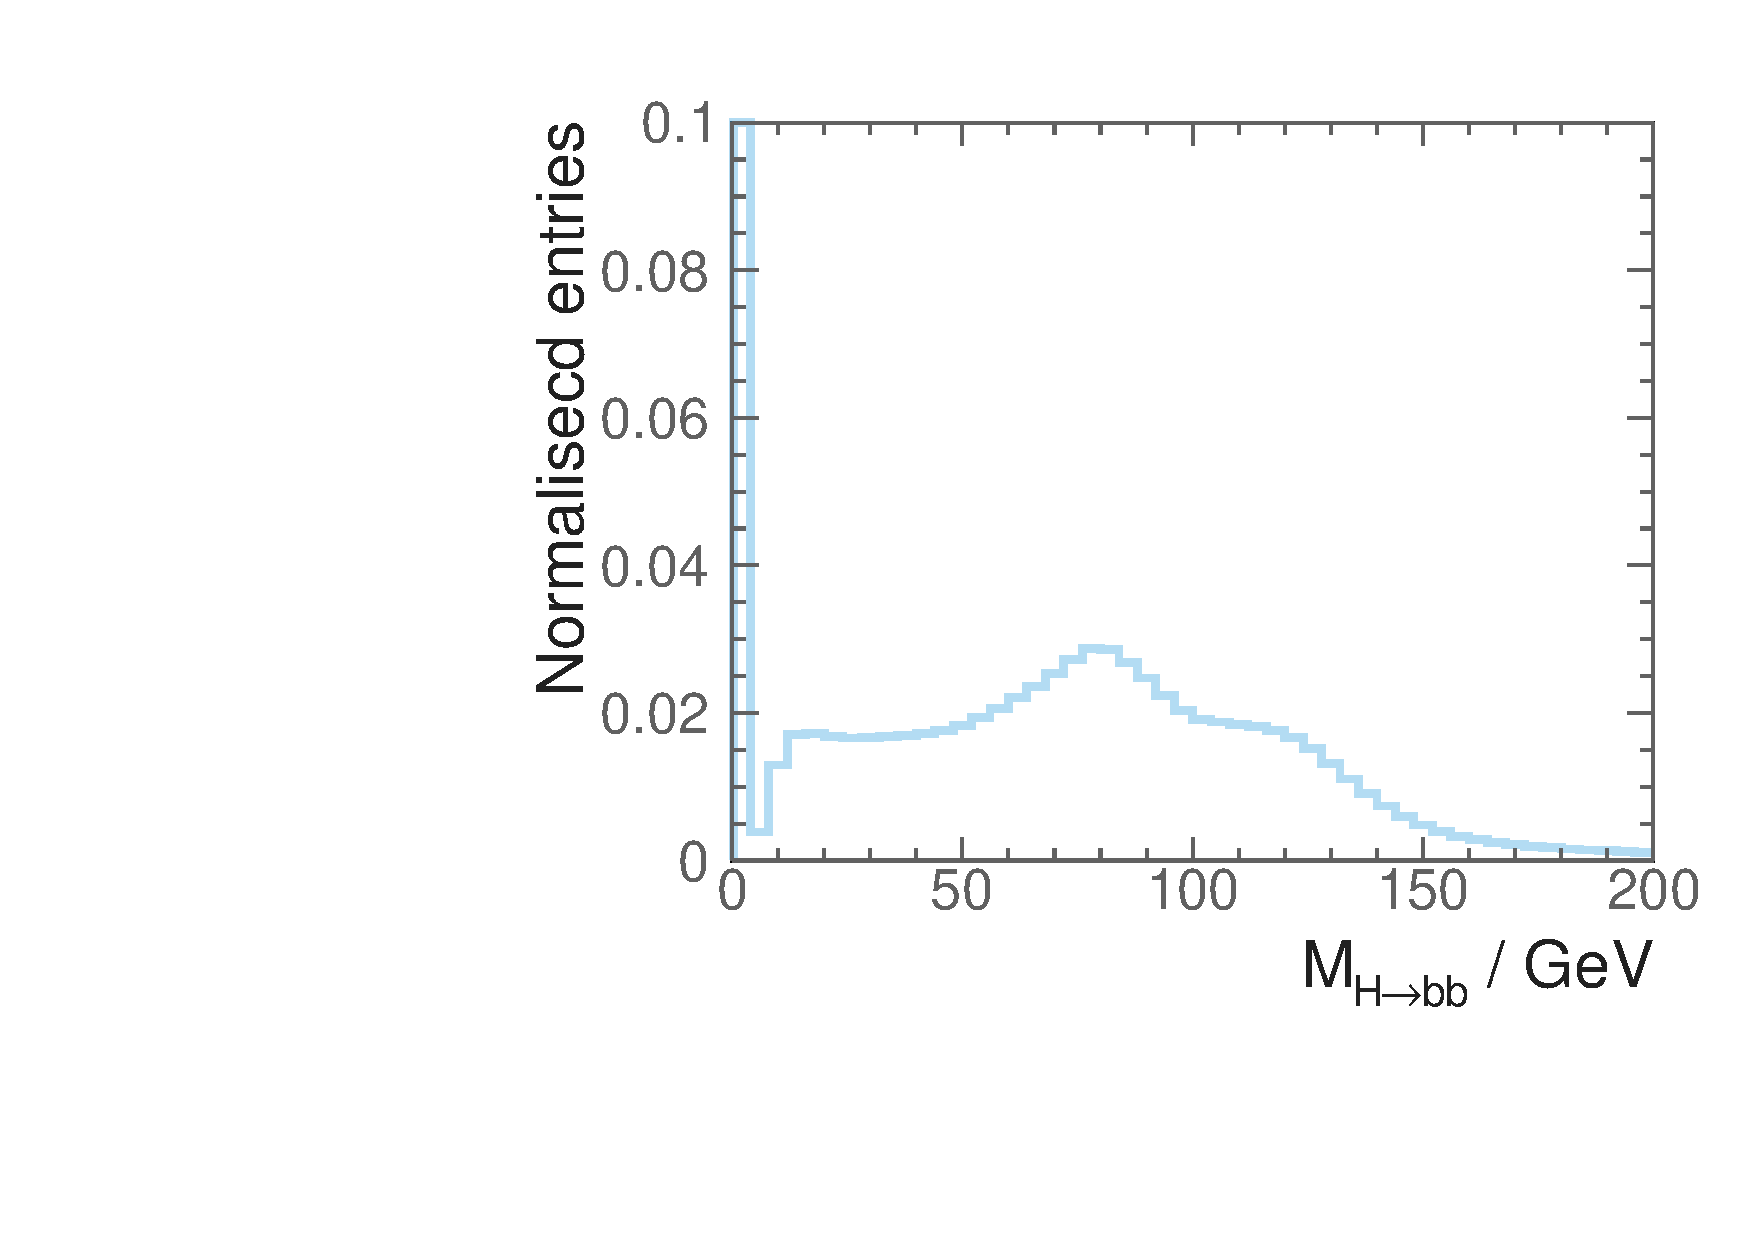
\includegraphics[width=\textwidth]{{doubleHiggs/jetPairing/nR0_7_6jet_btag2_Higgs1_M_TMVA20170223R0_7_qq_btag2_prepare_bkg}.pdf}
    \caption{Background}
   \label{fig:doubleHiggsJetPairingBackground}
  \end{subfigure}
\caption
   {The normalised distribution of $m_{\Hbb}$ after jet pairing, for a) signal channel, hadronic \WW decay of \eeToHHbbWW, b) sum of all background channels. All plots are shown for \rootS{1.4}.}
   \label{fig:doubleHiggsJetPairing}
\end{figure}


\begin{table}[!tbp]\centering
% TODO fix lumi correction for e gamma, gamma e
% TODO change some of sample cross section for  electron-photon interaction with four quarks and a neutrino final state
%\small{

\begin{tabular}{lrrrr}
\hline \hline
 \multicolumn{1}{m{3.5cm}}{Channel / Efficiency \rootS{1.4}} &  \multicolumn{1}{m{2cm}}{Expected number of events}  & \multicolumn{1}{m{1.5cm}}{Lepton evto} & \multicolumn{1}{m{1.5cm}}{Mutually exclusive} & \multicolumn{1}{m{1.5cm}}{Jet Pairing} \\
\hline
\eeToHH $\to$ \\
\HepProcess{ \Pbottom \APbottom \PWplus \PWminus \Pnue \APnue}, hadronic             &27.9& 89.7\% & 79.1\% & 78.3\%\\
\hline
\eeToHH $\to$ \\
\HepProcess{ \Pbottom \APbottom \Pbottom \APbottom \Pnue \APnue}             &67.6& 90.8\% & 18.0\% & 18.0\% \\
\eeToHH $\to$ other & 128.0 & 40.8\% & 35.8\% & 31.2\% \\
\hline
\eeTo{\qlight \qlight \PHiggs \Pnu \APnu}  & 1290 & 72.8\% & 69.7\% & 57.7\%\\
\eeTo{\Pcharm \APcharm \PHiggs \Pnu \APnu}  & 540 & 74.7\%& 59.8\%& 52.7\%\\
\eeTo{\Pbottom \APbottom \PHiggs \Pnu \APnu}  & 465 & 74.3\%& 32.2\%& 31.8\%\\

\eeTo{ \Pquark \Pquark \Pquark \Pquark}   &   1867650& 79.9\% & 64.0\%& 38.6\%\\
\eeTo{ \Pquark \Pquark \Pquark \Pquark \Plepton \Plepton}& 93150 & 8.9\%& 8.2\%& 4.7\%\\
\eeTo{ \Pquark \Pquark \Pquark \Pquark \Plepton \Pnu}& 165600 & 16.5\%& 14.6\%& 13.3\%\\
\eeTo{ \Pquark \Pquark \Pquark \Pquark \Pnu \APnu} & 34800& 87.6\%& 82.0\%& 46.8\%\\

\eeTo{ \Pquark \Pquark} &  6014250 & 81.0\%& 57.8\%& 39.0\%\\
\eeTo{ \Pquark \Pquark \Plepton \Pnu} &  6464550 & 22.5\%& 17.0\%& 10.5\%\\
\eeTo{ \Pquark \Pquark \Pl \Pl} &  4088700 & 19.4\%& 18.6\%& 12.4\%\\
\eeTo{ \Pquark \Pquark \Pnu \Pnu} & 1181550 & 91.8\%& 74.0\%& 47.3\% \\
\hline
\egamma{\Pepm}{\Pphoton}{\BS}{\Pepm \Pquark \Pquark \Pquark \Pquark} & 2606625  & 34.2\%& 33.5\%& 22.9\%\\
%\egamma{\Pem}{\Pphoton}{BS}{\Pem \Pquark \Pquark \Pquark \Pquark} & 1305787.5  & 34.0\%& 33.3\%& 22.8\%\\
%\egamma{\Pep}{\Pphoton}{BS}{\Pep \Pquark \Pquark \Pquark \Pquark} & 1300837.5 & 34.3\%& 33.6\%& 22.9\%\\
\egamma{\Pepm}{\Pphoton}{\EPA}{\Pepm \Pquark \Pquark \Pquark \Pquark} & 861000.0 & 16.4\%& 15.8\%& 10.7\%\\
%\egamma{\Pem}{\Pphoton}{EPA}{\Pem \Pquark \Pquark \Pquark \Pquark} & 430650.0 & 16.4\%& 15.8\%& 10.7\%\\
%\egamma{\Pep}{\Pphoton}{EPA}{\Pep \Pquark \Pquark \Pquark \Pquark}  & 430350.0 & 16.3\% & 15.8\%& 10.7\%\\
\egamma{\Pepm}{\Pphoton}{\BS}{\Pnu \Pquark \Pquark \Pquark \Pquark}& 178987.5  & 85.6\%& 81.3\%& 54.4\%\\
%\egamma{\Pem}{\Pphoton}{BS}{\Pnu \Pquark \Pquark \Pquark \Pquark}& 89775.0  & 85.6\%& 81.3\%& 54.7\%\\
%\egamma{\Pep}{\Pphoton}{BS}{\APnu \Pquark \Pquark \Pquark \Pquark}& 89212.5 &.85.6\% & 81.3\%& 54.0\%\\
\egamma{\Pepm}{\Pphoton}{\EPA}{\Pnu \Pquark \Pquark \Pquark \Pquark}& 52050  & 44.5\% & 42.0\%& 27.4\%\\
%\egamma{\Pem}{\Pphoton}{EPA}{\Pnu \Pquark \Pquark \Pquark \Pquark}& 26100.0  & 44.6\% & 42.1\%& 27.6\%\\
%\egamma{\Pep}{\Pphoton}{EPA}{\APnu \Pquark \Pquark \Pquark \Pquark}& 25950.0  & 44.4\%& 41.9\%& 27.2\% \\
\egamma{\Pepm}{\Pphoton}{\BS}{\Pquark \Pquark \PHiggs \Pnu} & 35437.5  & 70.7\% & 65.0\%& 55.4\%\\
%\egamma{\Pem}{\Pphoton}{BS}{\Pquark \Pquark \PHiggs \Pnu} & 17775  & 70.6\% & 64.9\%& 55.3\%\\
%\egamma{\Pep}{\Pphoton}{BS}{\Pquark \Pquark \PHiggs \Pnu} & 17662.5  & 70.7\% & 65.0\% & 55.5\%\\
\egamma{\Pepm}{\Pphoton}{\EPA}{\Pquark \Pquark \PHiggs \Pnu} & 10170  & 37.0\% & 33.8\% & 28.8\%\\
%\egamma{\Pem}{\Pphoton}{EPA}{\Pquark \Pquark \PHiggs \Pnu} & 5085  & 36.9\% & 33.7\% & 28.7\%\\
%\egamma{\Pep}{\Pphoton}{EPA}{\Pquark \Pquark \PHiggs \Pnu} & 5085   & 37.1\% & 33.9\% & 28.9\%\\
\hline
\gammagamma{\Pphoton}{\BS}{\Pphoton}{\BS}{ \Pquark \Pquark \Pquark \Pquark}& 2054951.5  & 85.6\%& 81.3\%& 54.0\%\\
\gammagamma{\Pphoton}{\BS}{\Pphoton}{\EPA}{ \Pquark \Pquark \Pquark \Pquark}& 4521037.5  &49.6\%& 48.5\%& 32.9\%\\
\gammagamma{\Pphoton}{\EPA}{\Pphoton}{\BS}{ \Pquark \Pquark \Pquark \Pquark}& 4539150 & 49.6\%& 48.5\%& 32.9\%\\
\gammagamma{\Pphoton}{\EPA}{\Pphoton}{\EPA}{ \Pquark \Pquark \Pquark \Pquark}& 1129500 & 31.0\% & 30.1\% & 20.5\%\\
\hline \hline
\end{tabular}

\caption
{Number of events and fraction of events passing lepton veto, the mutually exclusive cuts, and the jet pairing  for the signal and background events at \rootS{1.4}, assuming an integrated luminosity of 1500\,$fb^{-1}$. The selection efficiencies are presented in a ``flow'' fashion. Every selection cut contains all the cuts to the left of it.}
\label{tab:doubleHiggs1.4TeVPreslection}
\end{table}


\section{Pre-selection}
\label{sec:doubleHiggsPreSelection}

After the association of jets to candidate bosons are made under hypothesis that an event is signal, kinematic and topological variables can be calculated. A set of pre-selection cuts are placed to discard the phase space dominated by background events. Cuts on \pT, b-jet tag, and invariant mass of the double Higgs system are used.

Since both Higgs bosons are on mass shell,  the invariant mass of the double Higgs system is large. Consequently, a cut on $m_{\HH} > 150$\,GeV, as shown in \FIGURE{fig:doubleHiggs1.4PreSelmHH}, removes a small amount of signal events, but discard lots of  background events, especially  \HepProcess{\Gammagamma \to \Pquark \Pquark \Pquark \Pquark} events.

\begin{figure}[!tbp]
    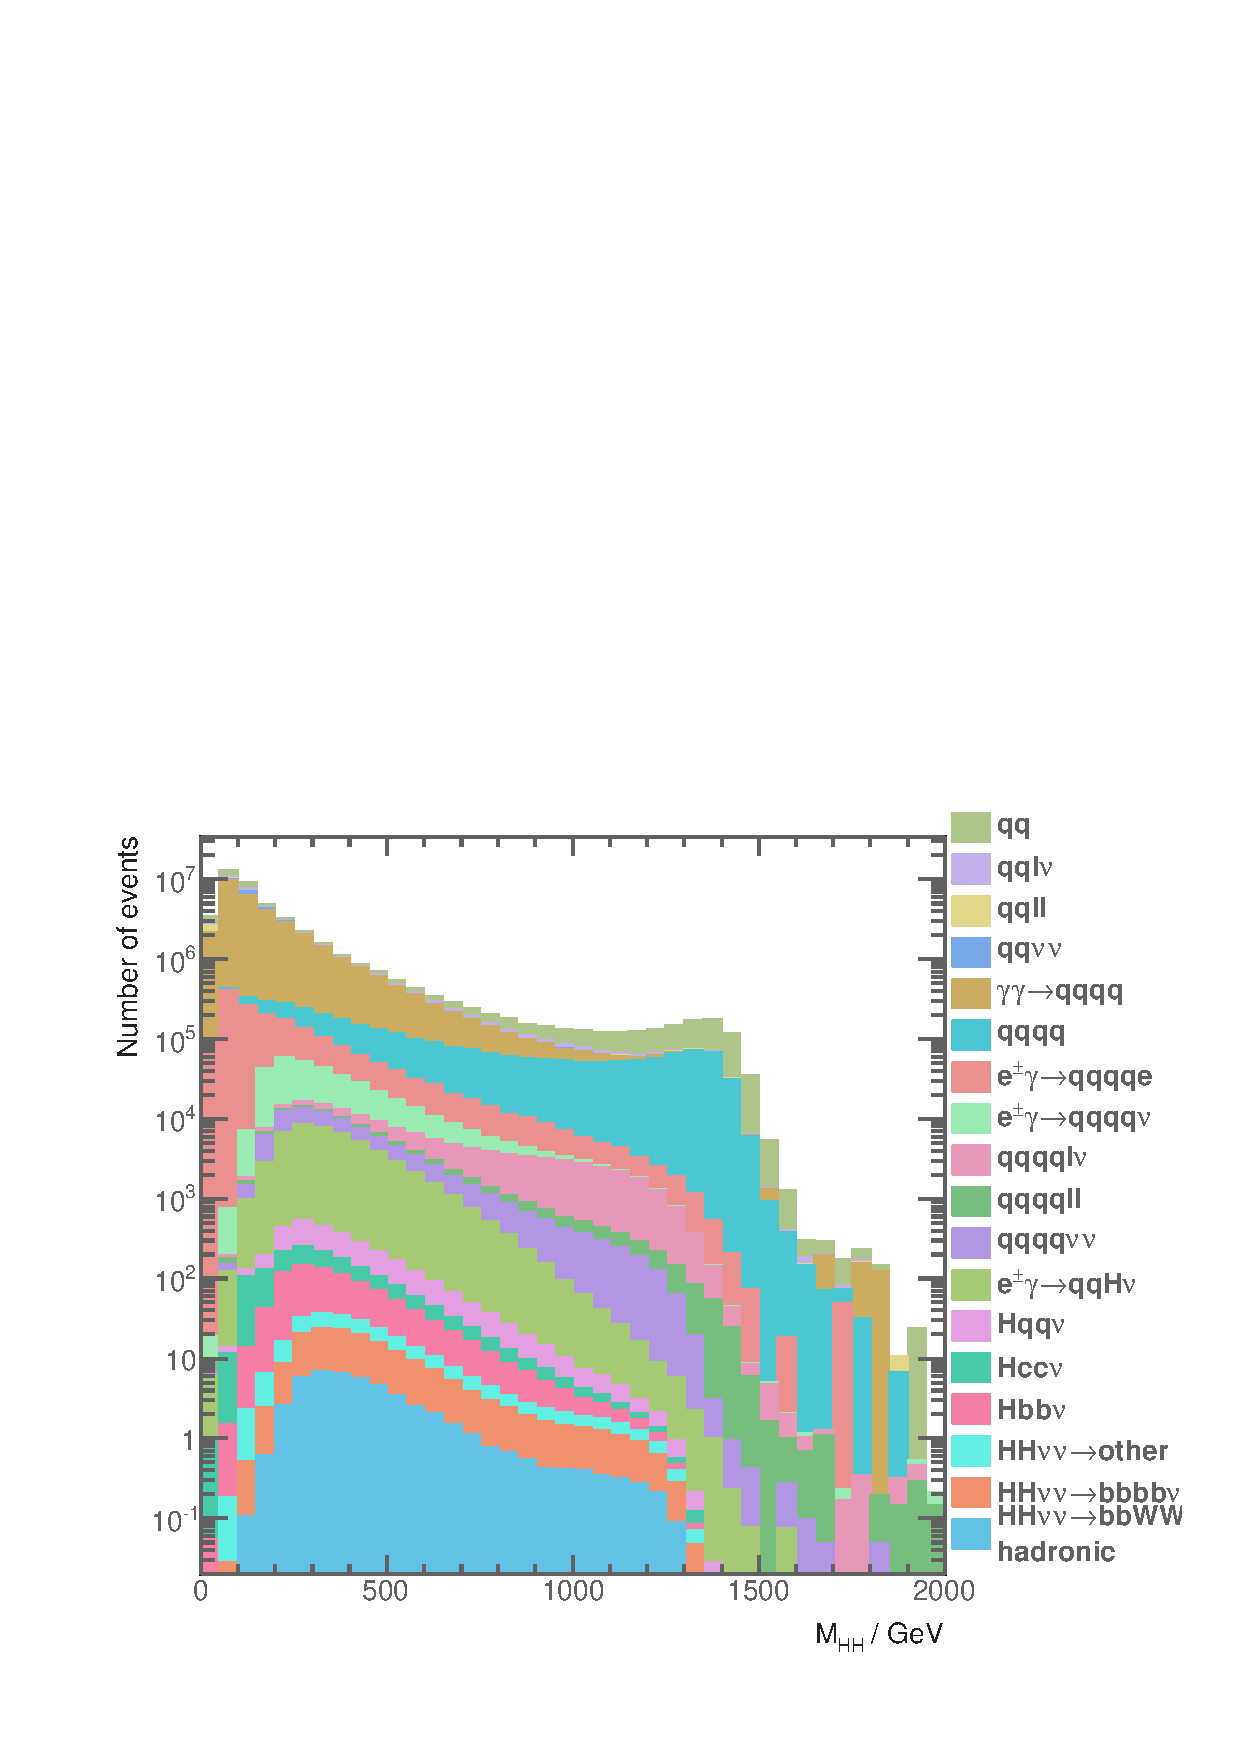
\includegraphics[width=0.95\textwidth]{{doubleHiggs/preSel/nR0_7_6jet_btag2_Higgs_all_M_TMVA20161208R0_7_qq_btag2_prepare}.pdf}
   \caption{Distributions of the invariant mass of the two Higgs system for \rootS{1.4}, assuming an intergraded luminosity of 1500\,\text{$fb^{-1}$}.}
    \label{fig:doubleHiggs1.4PreSelmHH}

\end{figure}


Many background events do not have b-quark jets in the final state. Therefore, by requiring the second highest b-jet tag value greater than 0.2, as shown in \FIGURE{fig:doubleHiggs1.4PreSelbtag},  background events with no b-jets in final states are removed.

\begin{figure}[!tbp]
    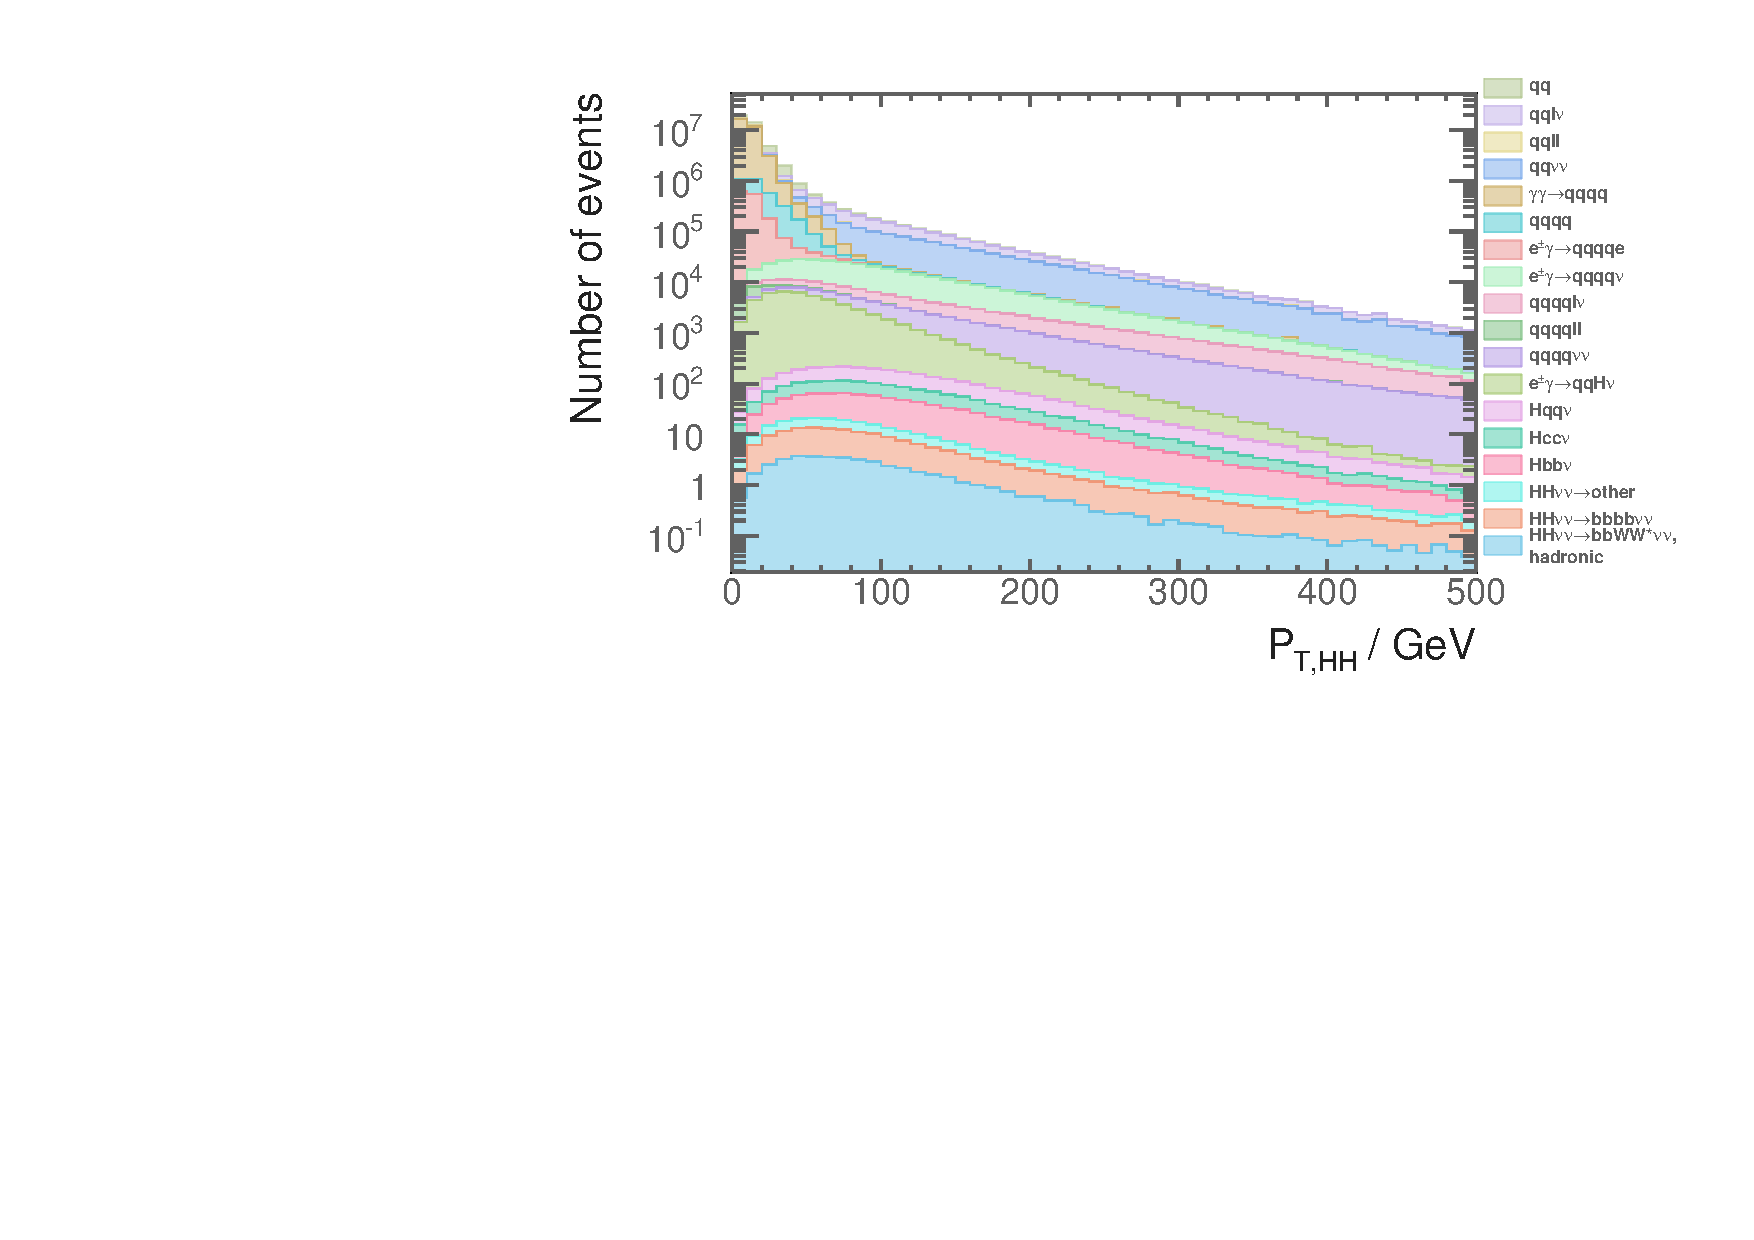
\includegraphics[width=0.95\textwidth]{{doubleHiggs/preSel/nR0_7_6jet_btag2_Higgs_all_Pt_TMVA20161208R0_7_qq_btag2_prepare}.pdf}

    \caption{Distributions of the  second highest b-jet tag value for \rootS{1.4}, assuming an intergraded luminosity of 1500\,\text{$fb^{-1}$}.}
    \label{fig:doubleHiggs1.4PreSelbtag}
\end{figure}

The signal final states have neutrinos and hence missing momentum in the events. Therefore, the transverse  momentum  of the two Higgs system is non zero. A cut of $\pT>30$\,GeV, as shown in \Figure{fig:doubleHiggs1.4PreSelpT}, is extremely effective against background channels with no neutrinos in the final state.

\begin{figure}[!tbp]
    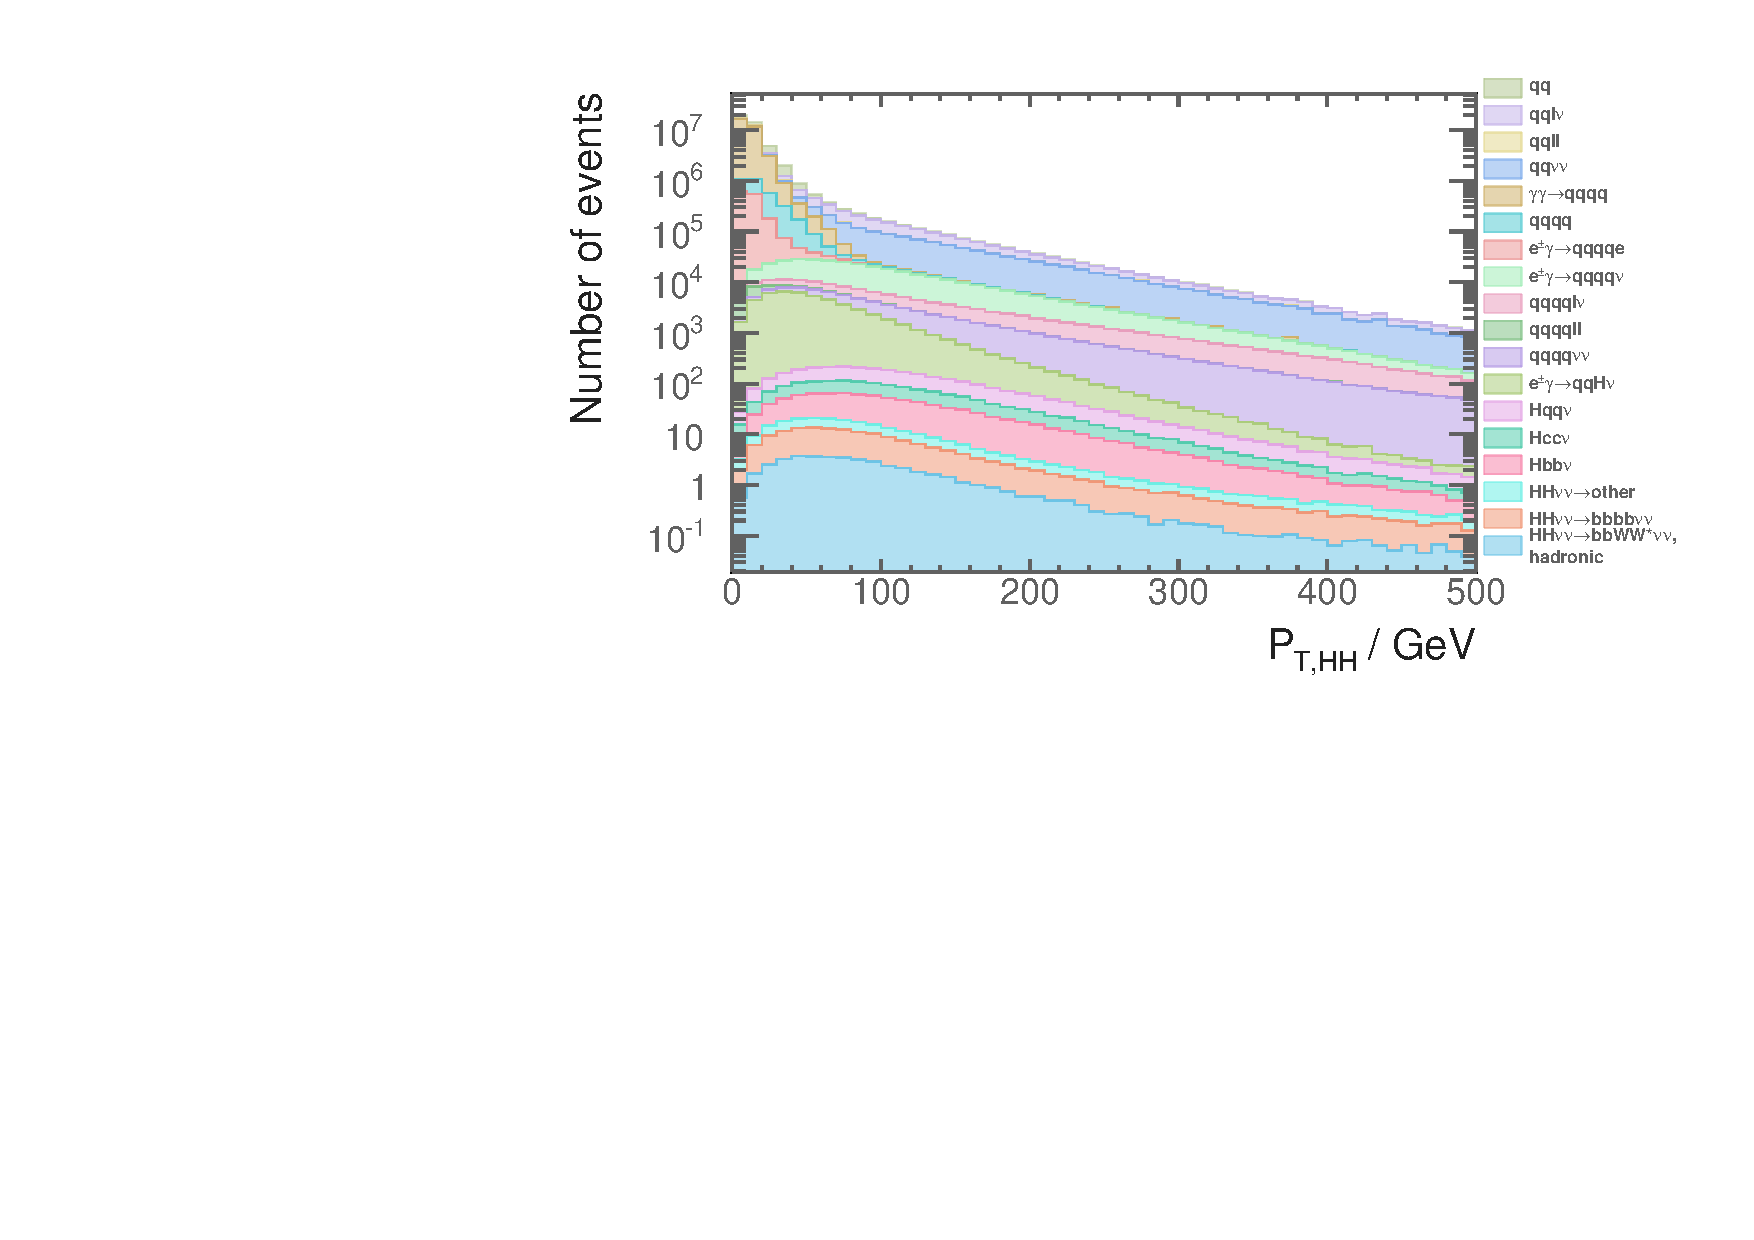
\includegraphics[width=0.95\textwidth]{{doubleHiggs/preSel/nR0_7_6jet_btag2_Higgs_all_Pt_TMVA20161208R0_7_qq_btag2_prepare}.pdf}

    \caption{Distributions of the transverse momentum  of the two Higgs system for \rootS{1.4}, assuming an intergraded luminosity of 1500\,\text{$fb^{-1}$}.}
    \label{fig:doubleHiggs1.4PreSelpT}
\end{figure}

The full list of fraction of events after each pre-selection cut can be found in \Table{tab:doubleHiggsPreslectionPart2}.

\begin{comment}
\begin{table}[!htbp]
\begin{tabular}{lr}
\hline
\hline
Pre-selection  &  \rootS{1.4}  \\
\hline
Discriminative pre-selection & \multicolumn{1}{R{0.5\textwidth}}{$m_{\HH} > 150\,GeV$, $B_2 > 0.2$,  $\pT_{\HH} > 30\,GeV$} \\
Loose cuts for MVA &  \multicolumn{1}{R{0.5\textwidth}}{$m_{\Hbb} < 500\,GeV$, $m_{\HWW} < 800\,GeV$, $m_{\PW} < 200\,GeV$, $m_{\HH} < 1400\,GeV$} \\
Mutually exclusive & \sumBtag{4} < 2.3, \y{34} < 3.7 \\
\hline
\hline
\end{tabular}
\caption
{Pre-selection cuts at \rootS{1.4}.}
\label{tab:doubleHiggsPreSel}
\end{table}
\end{comment}




\begin{table}[!tbp]\centering

\begin{tabular}{lrrr}
\hline \hline
 \multicolumn{1}{L{0.3\textwidth}}{Channel} &  \multicolumn{1}{R{0.2\textwidth}}{$m_{HH}$>150GeV}  & \multicolumn{1}{R{0.2\textwidth}}{$B_2$>0.2} & \multicolumn{1}{R{0.2\textwidth}}{\pT>30GeV}  \\
\hline
\eeToHH $\to$ \\
\HepProcess{ \Pbottom \APbottom \PWplus \PWminus \Pnue \APnue}, hadronic             & 78.1\%& 66.3\% & 59.7\% \\
\hline
\eeToHH $\to$ \\
\HepProcess{ \Pbottom \APbottom \Pbottom \APbottom \Pnue \APnue}             &17.8\%& 17.4\% & 15.4\%  \\
\eeToHH $\to$ other & 30.5\% &23.0\% & 20.5\%  \\
\hline
\eeTo{\qlight \qlight \PHiggs \Pnu \APnu}  & 56.8\% &42.3\% & 39.5\% \\
\eeTo{\Pcharm \APcharm \PHiggs \Pnu \APnu}  & 44.8\% & 34.1\% & 31.7\%\\
\eeTo{\Pbottom \APbottom \PHiggs \Pnu \APnu}  & 30.7\% &27.0\% & 25.2\%\\

\eeTo{ \Pquark \Pquark \Pquark \Pquark}   & 36.1\%  &13.2\% & 3.4\%\\
\eeTo{ \Pquark \Pquark \Pquark \Pquark \Plepton \Plepton}& 4.7\% &1.5\% & 0.3\%\\
\eeTo{ \Pquark \Pquark \Pquark \Pquark \Plepton \Pnu}& 13.2\%. &10.7\% & 9.8\%\\
\eeTo{ \Pquark \Pquark \Pquark \Pquark \Pnu \APnu} & 46.1\% &17.7\% & 16.6\%\\

\eeTo{ \Pquark \Pquark} &  8.1\% &3.7\% & 0.8\%\\
\eeTo{ \Pquark \Pquark \Plepton \Pnu} & 3.1\% & 1.2\% & 0.9\%\\
\eeTo{ \Pquark \Pquark \Pl \Pl} &  0.7\% &0.4\% & 0.1\%\\
\eeTo{ \Pquark \Pquark \Pnu \Pnu} & 9\% & 4.3\% & 4.0\%\\
\hline
\egamma{\Pepm}{\Pphoton}{\BS}{\Pepm \Pquark \Pquark \Pquark \Pquark} & 10.1\% & 4.1\%  & 0.4\%\\
%\egamma{\Pem}{\Pphoton}{BS}{\Pem \Pquark \Pquark \Pquark \Pquark} & 10.1\%  & 4.1\% 0.3\\
%\egamma{\Pep}{\Pphoton}{BS}{\Pep \Pquark \Pquark \Pquark \Pquark} & 10.1\% & 4.1\% & 0.4\%\\
\egamma{\Pepm}{\Pphoton}{\EPA}{\Pepm \Pquark \Pquark \Pquark \Pquark} & 5.1\% & 2.0\% & 0.3\%\\
%\egamma{\Pem}{\Pphoton}{EPA}{\Pem \Pquark \Pquark \Pquark \Pquark} & 5.1\% & 2.0\% & 0.2\%\\
%\egamma{\Pep}{\Pphoton}{EPA}{\Pep \Pquark \Pquark \Pquark \Pquark}  & 5.0\% & 2.0\% & 0.3\% \\
\egamma{\Pepm}{\Pphoton}{\BS}{\Pnu \Pquark \Pquark \Pquark \Pquark}& 53.0\%  & 28.0\% & 25.1\%\\
%\egamma{\Pem}{\Pphoton}{BS}{\Pnu \Pquark \Pquark \Pquark \Pquark}& 53.3\% & 28.3\%  & 25.3\%\\
%\egamma{\Pep}{\Pphoton}{BS}{\APnu \Pquark \Pquark \Pquark \Pquark}& 52.6\% & 27.7\% & 24.9\% \\
\egamma{\Pem}{\Pphoton}{\EPA}{\Pnu \Pquark \Pquark \Pquark \Pquark}& 26.7\% & 13.8\% & 12.5\% \\
%\egamma{\Pem}{\Pphoton}{EPA}{\Pnu \Pquark \Pquark \Pquark \Pquark}&  26.9\% & 13.9\% & 12.6\% \\
%\egamma{\Pep}{\Pphoton}{EPA}{\APnu \Pquark \Pquark \Pquark \Pquark}& 26.5\% & 13.6\%  & 12.3\% \\
\egamma{\Pepm}{\Pphoton}{\BS}{\Pquark \Pquark \PHiggs \Pnu} & 54.3\% & 40.3\%  & 30.6\% \\
%\egamma{\Pem}{\Pphoton}{BS}{\Pquark \Pquark \PHiggs \Pnu} & 54.2\% & 40.2\%  & 30.6\% \\
%\egamma{\Pep}{\Pphoton}{BS}{\Pquark \Pquark \PHiggs \Pnu} & 54.4\% & 40.4\% & 30.6\%  \\
\egamma{\Pem}{\Pphoton}{\EPA}{\Pquark \Pquark \PHiggs \Pnu} & 28.2\% & 20.9\% & 16.1\%  \\
%\egamma{\Pem}{\Pphoton}{EPA}{\Pquark \Pquark \PHiggs \Pnu} & 28.1\% & 20.9\% & 16.0\%  \\
%\egamma{\Pep}{\Pphoton}{EPA}{\Pquark \Pquark \PHiggs \Pnu} & 28.3\% & 20.9\%   & 16.1\%  \\
\hline
\gammagamma{\Pphoton}{\BS}{\Pphoton}{\BS}{ \Pquark \Pquark \Pquark \Pquark}& 23.1\% & 9.2\%  & 0.3\%\\
\gammagamma{\Pphoton}{\BS}{\Pphoton}{\EPA}{ \Pquark \Pquark \Pquark \Pquark}& 13.6\% & 5.4\%  &0.4\%\\
\gammagamma{\Pphoton}{\EPA}{\Pphoton}{\BS}{ \Pquark \Pquark \Pquark \Pquark}& 13.6\% & 5.4\% & 0.3\%\\
\gammagamma{\Pphoton}{\EPA}{\Pphoton}{\EPA}{ \Pquark \Pquark \Pquark \Pquark}& 8.6\% & 3.5\% & 0.3\% \\
\hline \hline
\end{tabular}
\caption[List of signal and background samples after pre-selection cuts at \rootS{1.4}.]
{List of signal and background events after each pre-selection cut at \rootS{1.4}.  The selection efficiencies are presented in a ``flow'' fashion. Every selection cut contains all the cuts to the left of it and all  cuts in \Table{tab:doubleHiggs1.4TeVPreslection} .}
\label{tab:doubleHiggsPreslectionPart2}
\end{table}


\begin{comment}
    const TCut selectionCut3000 = "tR0_7_6jet_btag2_ChiSquared<20  && TightIsoLepTauAll_nPfo < 1 && BonoForwardElectronPhotons_nPfo < 1 && \
         tR0_7_6jet_btag2_Higgs_all_M>150  && \
       tR0_7_4jet_btag2_Higgs_all_bTag < 2.3 && tR0_7_6jet_btag2_minusLogY34 < 3.7 \
       && tR0_7_6jet_btag2_bTag1 > 0.7 &&\
        tR0_7_6jet_btag2_Higgs_all_M  < 3000 &&  tR0_7_6jet_btag2_Higgs1_M < 500 &&  tR0_7_6jet_btag2_Higgs2_M < 800 &&  tR0_7_6jet_btag2_W_Onshell_M < 200";

    const TCut selectionCut1400 = "nR0_7_6jet_btag2_ChiSquared<20  && IsoLepTauAll_nPfo < 1      && BonoForwardElectronPhotons_nPfo < 1 && nR0_7_6jet_btag2_Higgs_all_M>150 && \
        nR0_7_4jet_btag2_Higgs_all_bTag < 2.3  && nR0_7_6jet_btag2_minusLogY34 < 3.6 \
        &&  nR0_7_6jet_btag2_bTag2 > 0.2 && nR0_7_6jet_btag2_Higgs_all_Pt> 30 &&\
        nR0_7_6jet_btag2_Higgs_all_M  < 1400 &&  nR0_7_6jet_btag2_Higgs1_M < 500 &&  nR0_7_6jet_btag2_Higgs2_M < 800 &&  nR0_7_6jet_btag2_W_Onshell_M < 200";
\end{comment}


\section{MVA variables}

Having extracted information about leptons, b-jets, and jet pairing, a number of variables are used to differentiate the signal and the background events. These variables are the basis of the subsequent MVA event selection. The variables used are listed in \Table{tab:doubleHiggsVaraibles}. The distributions of the four most power discriminators are show in \Figure{fig:doubleHiggs1.4var}.

\subsection{Invariant mass  variables}

Four invariant masses are used in the MVA event selection: the invariant mass of  \Hbb ($m_{\Hbb}$), the invariant mass of  \HWW ($m_{\HWW}$), the invariant mass of  \PW ($m_{\PW}$), and the invariant mass of the double Higgs system ($m_{\HH}$).

After the jet pairing under the hypothesis of the signal events, the distributions of the invariant mass of the physical bosons of the signal events have peaks around the expect masses, where the distributions of the  background events do not have such resonance structure. Shown in the \Figure{fig:doubleHiggs1.4varMHbb} (also similar plots can be found in the jet pairing section), the distributions of the invariant mass of the \Hbb is  different to the distributions of the background events. Similarly, the distributions of the invariant mass of the \HWW, shown in \Figure{fig:doubleHiggs1.4varMHWW} have different peak position to the distributions of the background events.  The invariant mass of the double Higgs system in the signal events is large due to the presence of two on-mass-shell Higgs bosons, which is also different to the distribution of the background events

\subsection{Energy and momentum variables}

Six energy and momentum variables participate in the MVA event selection: the energy of the off-mass-shell \PW ($E_{\W*}$), the energy of the missing momenta ($E_{mis}$), the transverse momentum of \Hbb ($\pT_{\Hbb}$), the transverse momentum of \HWW ($\pT_{\HWW}$), the transverse momentum of \PW ($\pT_{\PW}$), and the transverse momentum of the double Higgs system ($\pT_{\HH}$).

For the off-mass-shell \PW, the energy  is used instead of the invariant mass, as invariant mass distribution of \W* does not have a resonance structure. The energy of the missing momenta is powerful against background events with no neutrinos in the final state. The missing momenta is calculated by assuming the collision at \sqrtS and a beam crossing angle of 20\,mrad. Other momentum variables correspond to the same physical bosons or the double Higgs system used in  the invariant mass  variables, for the same reason that the distributions of these momentum variables are different for the signal events and the background events.


\subsection{Lab-frame angle variables}

Four lab-frame angle variables are in the MVA event selection: the pseudorapidity of the missing momenta ($\eta_{mis}$), the  acollinearity of the two jets associated with \Hbb ($\acolinearity{\Hbb}$),  the  acollinearity of the two jets associated with \HWW ($\acolinearity{\HWW}$), and the  acollinearity of the two Higgs bosons($\acolinearity{\HH}$).

The pseudorapidity   of the missing momenta is used instead of the polar angle is because the forward polar angles are transformed to a larger range in the pseudorapidity. The pseudorapidity of the missing momenta is defined as
\begin{equation}
\eta_{mis} \equiv  - \ln \left[ \tan \left( \frac{\theta_{mis}}{2} \right) \right],
\end{equation}
where $\theta_{mis}$ is the polar angle of the missing momenta measured in a spherical polar coordinate system.

Acollinearity is a measures the angle between the two momenta. The definition for the acollinearity for momenta $i$ and momenta $j$ is
\begin{equation}
\acolinearity{ij} = \pi - \cos^{-1}\left(\textbf{\^{p}}_i\cdot\textbf{\^{p}}_j\right),
\end{equation}
where $\textbf{\^{p}}_i$ is the unit momentum three-vector of momenta $i$. The distribution of the \acolinearity{\Hbb}, shown in \Figure{fig:doubleHiggs1.4varAcolHbb}, peaks at the value of 0 or $\pi$ for many background events, which are not the same as the signal events. For the same reason, the distributions of $\acolinearity{\HWW}$ and $\acolinearity{\HH}$ are different for the signal and the background events.

\subsection{Boosted-frame angle variables}

The MVA event selection also uses five boosted-frame angle variables: the angle between two jets associated with \Hbb in the \Hbb decay rest frame ($\cosStar{\Hbb}$), the angle between two \PW associated with \HWW in the \HWW decay rest frame ($\cosStar{\HWW}$), the angle between two jets associated with \PW in the \PW decay rest frame ($\cosStar{\PW}$), the angle between two jets associated with \W* in the \W* decay rest frame ($\cosStar{\W*}$), and the angle between two Higgs bosons in two Higgs bosons decay rest frame ($\cosStar{\HH}$).

These variables are some of the most powerful variables. For example, $\cosStar{\Hbb}$ for  the signal events has a unform distribution, shown in \Figure{fig:doubleHiggs1.4varSpinHbb}, as it is equally likely for two quarks to decay in any open angle in the \Hbb decay rest frame. For the background events, by pairing jets under the signal event hypothesis, $\cosStar{\Hbb}$ does not have a flat distribution. The  $\cosStar{\Hbb}$ for the background events peaks at 1.

\subsection{Event shape variables}

Five event shapes variables are used in the MVA event selection: the absolute value of the sphericity ($\abs{\sphericity}$), the negative logarithm of \y{23} ($-\ln(\y{23})$), the negative logarithm of \y{34} ($-\ln(\y{34})$), the negative logarithm of \y{45} ($-\ln(\y{45})$), the negative logarithm of \y{56} ($-\ln(\y{56})$).

The sphericity, \sphericity, is a measurement of the spherically symmetry of the event, which will be different for the signal and background events. The sphericity is  derived from the sphericity tensor \cite{PhysRevLett.35.1609}. The sphericity tensor is  defined as
\begin{equation}
{\bm{S}^{\alpha\beta}} = \frac{\sum_{i}p^{\alpha}_{i}p^{\beta}_{i}}{\sum_{i}\absOf{\vec{p_{i}}}^2},
\end{equation}
where $\vec{p_{i}}$ is the momentum vector of the particle $i$. Summation is over all particles in the event. $\alpha$ and $\beta$ refer to the x, y, z coordinate axis. Eigenvalues of $\bm{S}$  tensor, denoted with $\lambda_{1}$, $\lambda_{2}$, $\lambda_{3}$, can be found via diagonalisation of the matrix $\bm{S}$. The normalisation condition requires $\lambda_{1}\!\geqslant\! \lambda_{2} \! \geqslant \! \lambda_{3}$ and $ \lambda_{1} \! + \! \lambda_{2} \! + \! \lambda_{3} \! = \! 1 $. Sphericity, $S$, is defined in terms of $\lambda$,
\begin{equation}
\sphericity = \frac{3}{2}\parenths{\lambda_{1} \! + \! \lambda_{2}}.
\end{equation}
\sphericity, is 0 for a perfect pencil-like back-to-back two-jet event, and 1 for a perfect spherically symmetric event.

The \y{} parameter is a measure of the number of jets in an event.  It describes the transition of  the exclusive jet algorithm going from $N$ clustered jets to $N\!+\!1$ clustered jets. For example, $\y{23}$ would be the $d_{cut}$ value for a exclusive jet algorithm, above which the jet algorithm returns 2 jets, below which the jet algorithm returns 3 jets. Numerically the \y{} parameter is often much smaller than 1. A typically way to convert the small number to a machine acceptable range is to take the negative logarithm of the number. See \Section{sec:pandoraJetAlg} for discussion on jet algorithms and $d_{cut}$.

\subsection{\Pbottom and \Pcharm tag  variables}

Six b-jet and c-jet tag variables are used in the MVA event selection: the highest b-jet tag value of the two jets associated with \Hbb ($\btagFull{1,\Hbb}$), the lowest b-jet tag value of the two jets associated with \Hbb ($\btagFull{2,\Hbb}$), the highest b-jet tag value of the two jets associated with \PW ($\btagFull{1,\PW}$), the highest b-jet tag value of the two jets associated with \W* ($\btagFull{1,\W*}$), the highest c-jet tag value of the two jets associated with \Hbb ($\ctagFull{1,\Hbb}$), and the highest c-jet tag value of the two jets associated with \PW ($\ctagFull{1,\PW}$).

As mentioned in the flavour tagging section, these b-jet and c-jet tag variables are useful to separate the signal events from the background events which do not have b-quark jets in the final states.

\subsection{\PFOs number  variables}

The last four variables used in the MVA event selection are the \PFOs number  variables: the number of \PFOs associated with \Hbb (\Hbb), the number of \PFOs associated with \HWW (\HWW), the number of \PFOs associated with \PW (\PW), the number of \PFOs associated with \W* (\W*). These variables are effective to differentiate the signal events from the background events with fewer than six quarks in final states.

An optimal set of 32 variables are chosen for the best MVA performance, whilst no strong ($>80\%$) pair-wise correlation exists between any two variables. %shown in \Figure{fig:doubleHiggs1.4Corr}.

 \begin{table}[!tbp]\centering
\begin{tabular}{lr}
\hline
\hline
Category &  Variable \\
\hline
Invariant mass &  \multicolumn{1}{R{0.6\textwidth}}{$m_{\Hbb}$, $m_{\HWW}$, $m_{\PW}$, $m_{\HH}$} \\
Energy and momentum & \multicolumn{1}{R{0.6\textwidth}}{$E_{\W*}$, $E_{mis}$, $\pT_{\Hbb}$, $\pT_{\HWW}$, $\pT_{\PW}$, $\pT_{\HH}$} \\
Lab-frame angles & \multicolumn{1}{R{0.6\textwidth}}{$\eta_{mis}$, $\acolinearity{\Hbb}$, $\acolinearity{\PW}$, $\acolinearity{\HH}$} \\
Boosted-frame angles & \multicolumn{1}{R{0.6\textwidth}}{$\cosStar{\Hbb}$, $\cosStar{\HWW}$, $\cosStar{\PW}$, $\cosStar{\W*}$, $\cosStar{\HH}$} \\
Event shape & \multicolumn{1}{R{0.6\textwidth}}{$\abs{\sphericity}$, $-\ln(\y{23})$, $-\ln(\y{34})$, $-\ln(\y{45})$, $-\ln(\y{56})$} \\
\Pbottom and \Pcharm tag & \multicolumn{1}{R{0.6\textwidth}}{$\btagFull{1,\Hbb}$, $\btagFull{2,\Hbb}$, $\btagFull{1,\PW}$, $\btagFull{1,\W*}$, $\ctagFull{1,\Hbb}$, $\ctagFull{1,\PW}$} \\
 \PFOs number &  \multicolumn{1}{R{0.6\textwidth}}{$\npfo{\Hbb}$, $\npfo{\HWW}$, $\npfo{\PW}$, $\npfo{\W*}$} \\
\hline
\hline
\end{tabular}
\caption
{Variables used in the MVA event selection for \rootS{1.4}}
\label{tab:doubleHiggsVaraibles}
\end{table}



 \begin{figure}[!tbp]
  \begin{subfigure}[b]{0.45\textwidth}
    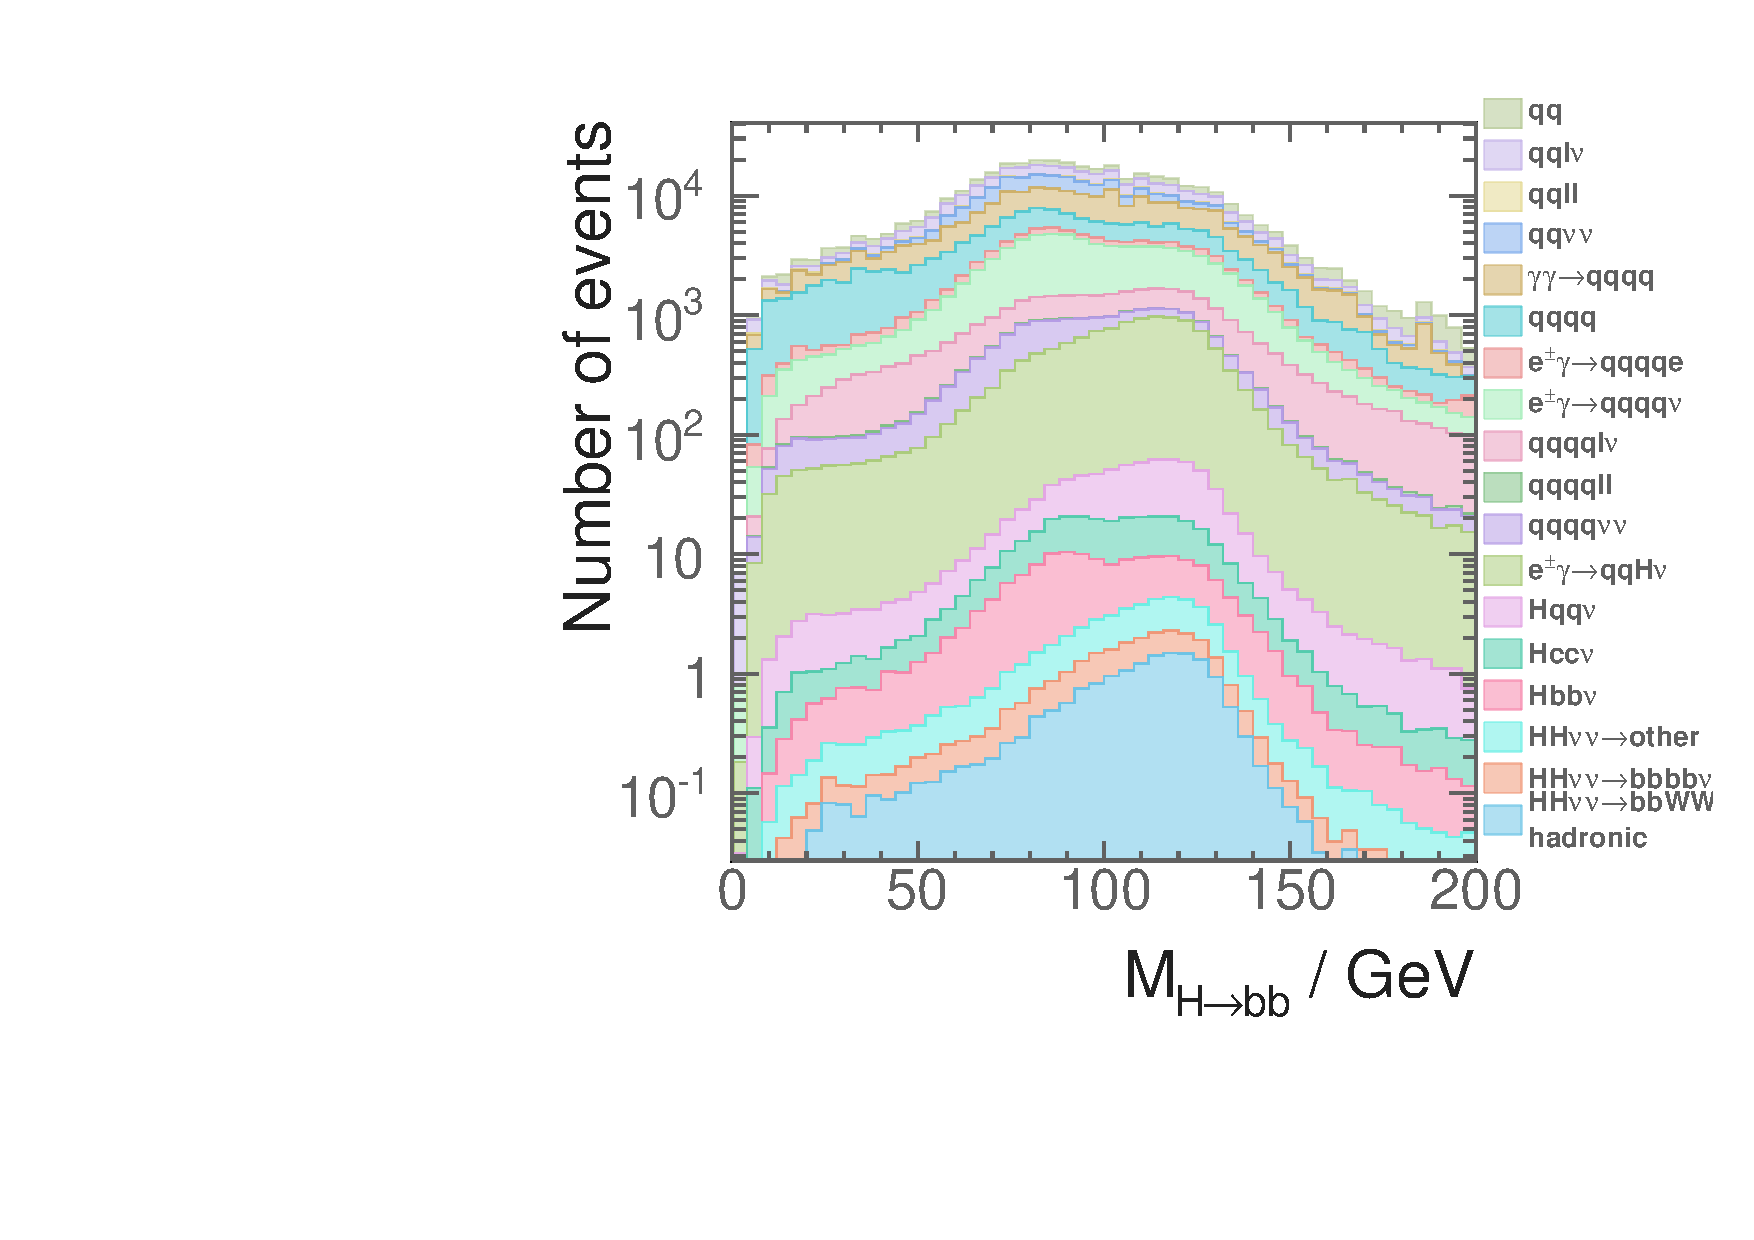
\includegraphics[width=\textwidth]{{doubleHiggs/1400var/nR0_7_6jet_btag2_Higgs1_M_TMVA20161208R0_7_qq_btag2_prepare_testNew2}.pdf}
    \caption{}
    \label{fig:doubleHiggs1.4varMHbb}
  \end{subfigure}
    \begin{subfigure}[b]{0.45\textwidth}
    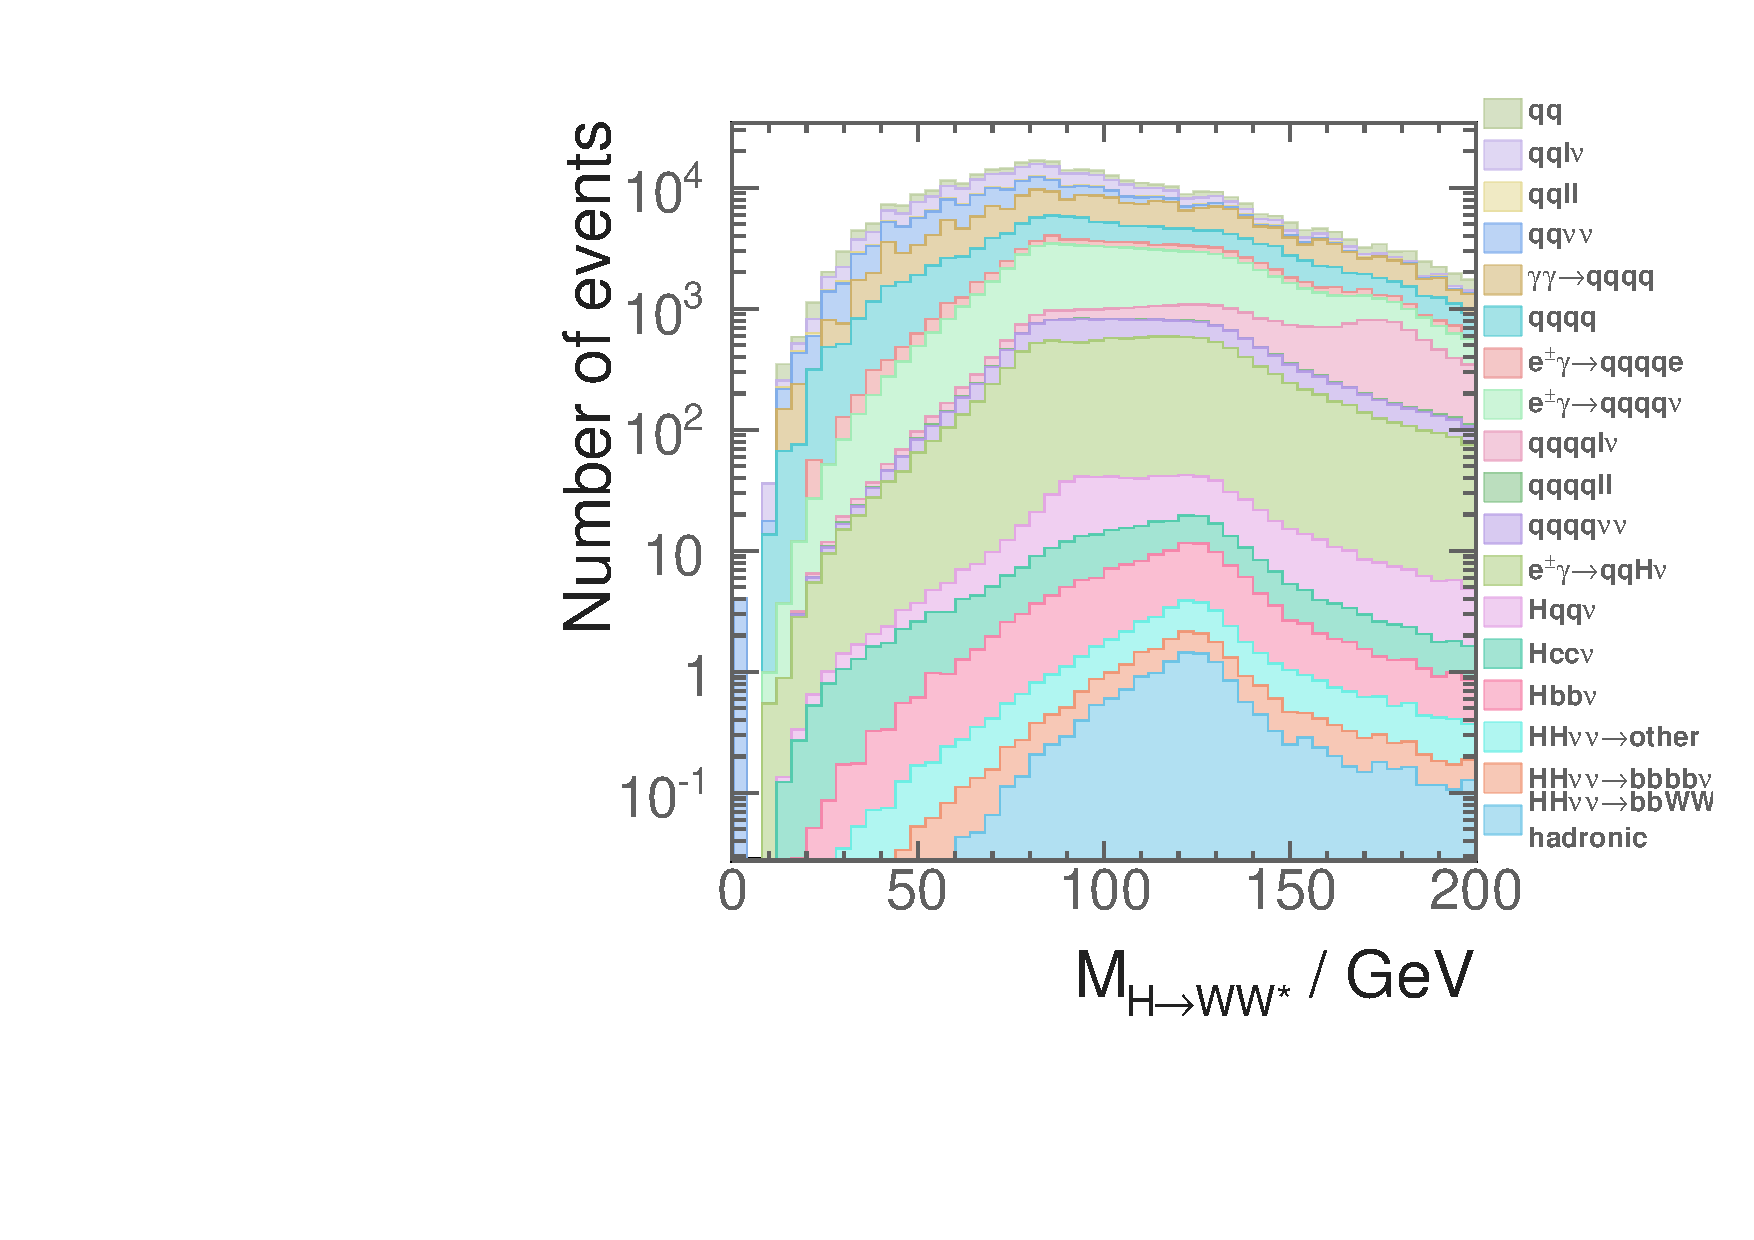
\includegraphics[width=\textwidth]{{doubleHiggs/1400var/nR0_7_6jet_btag2_Higgs2_M_TMVA20161208R0_7_qq_btag2_prepare_testNew2}.pdf}
    \caption{}
    \label{fig:doubleHiggs1.4varMHWW}
  \end{subfigure}
    \begin{subfigure}[b]{0.45\textwidth}
    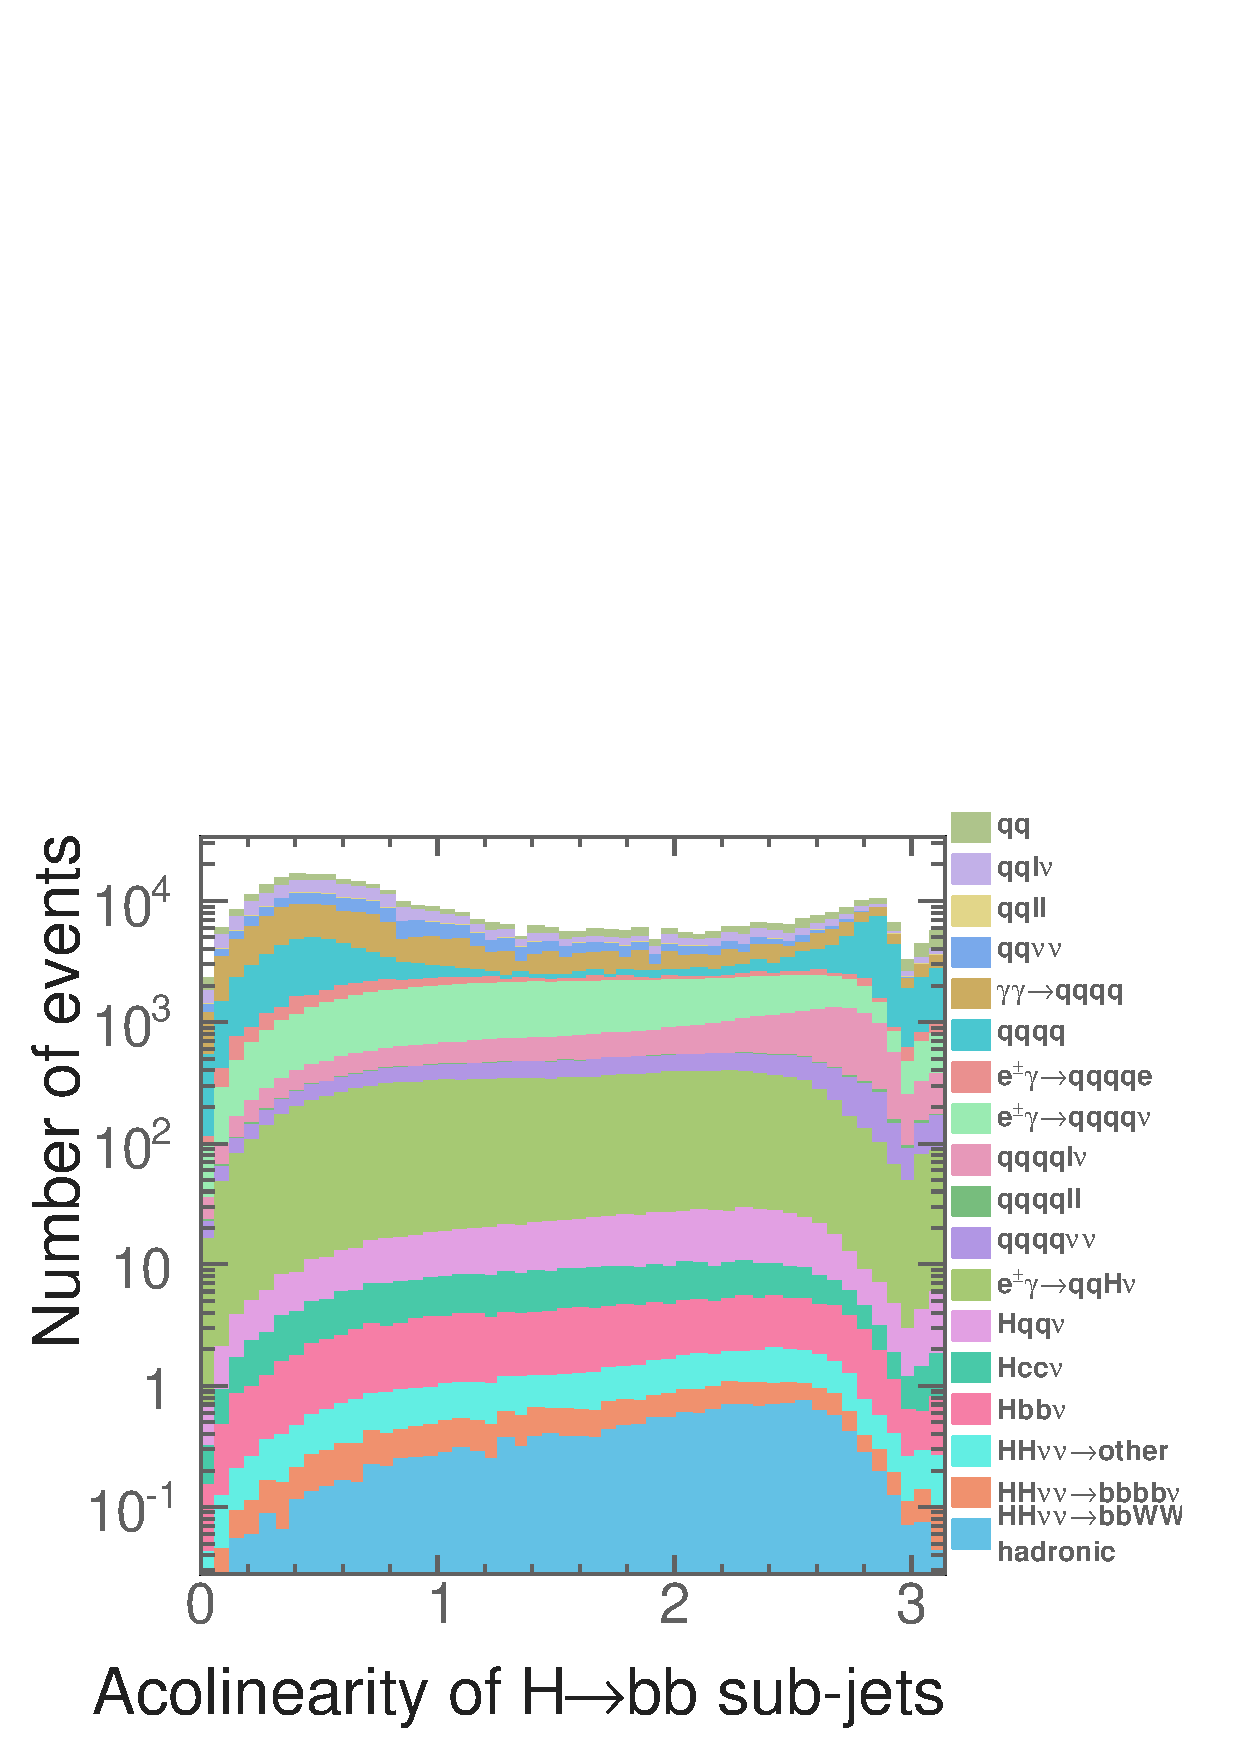
\includegraphics[width=\textwidth]{{doubleHiggs/1400var/nR0_7_6jet_btag2_Higgs1_acolinearity_TMVA20161208R0_7_qq_btag2_prepare_testNew2}.pdf}
    \caption{}
    \label{fig:doubleHiggs1.4varAcolHbb}
  \end{subfigure}
    \begin{subfigure}[b]{0.45\textwidth}
    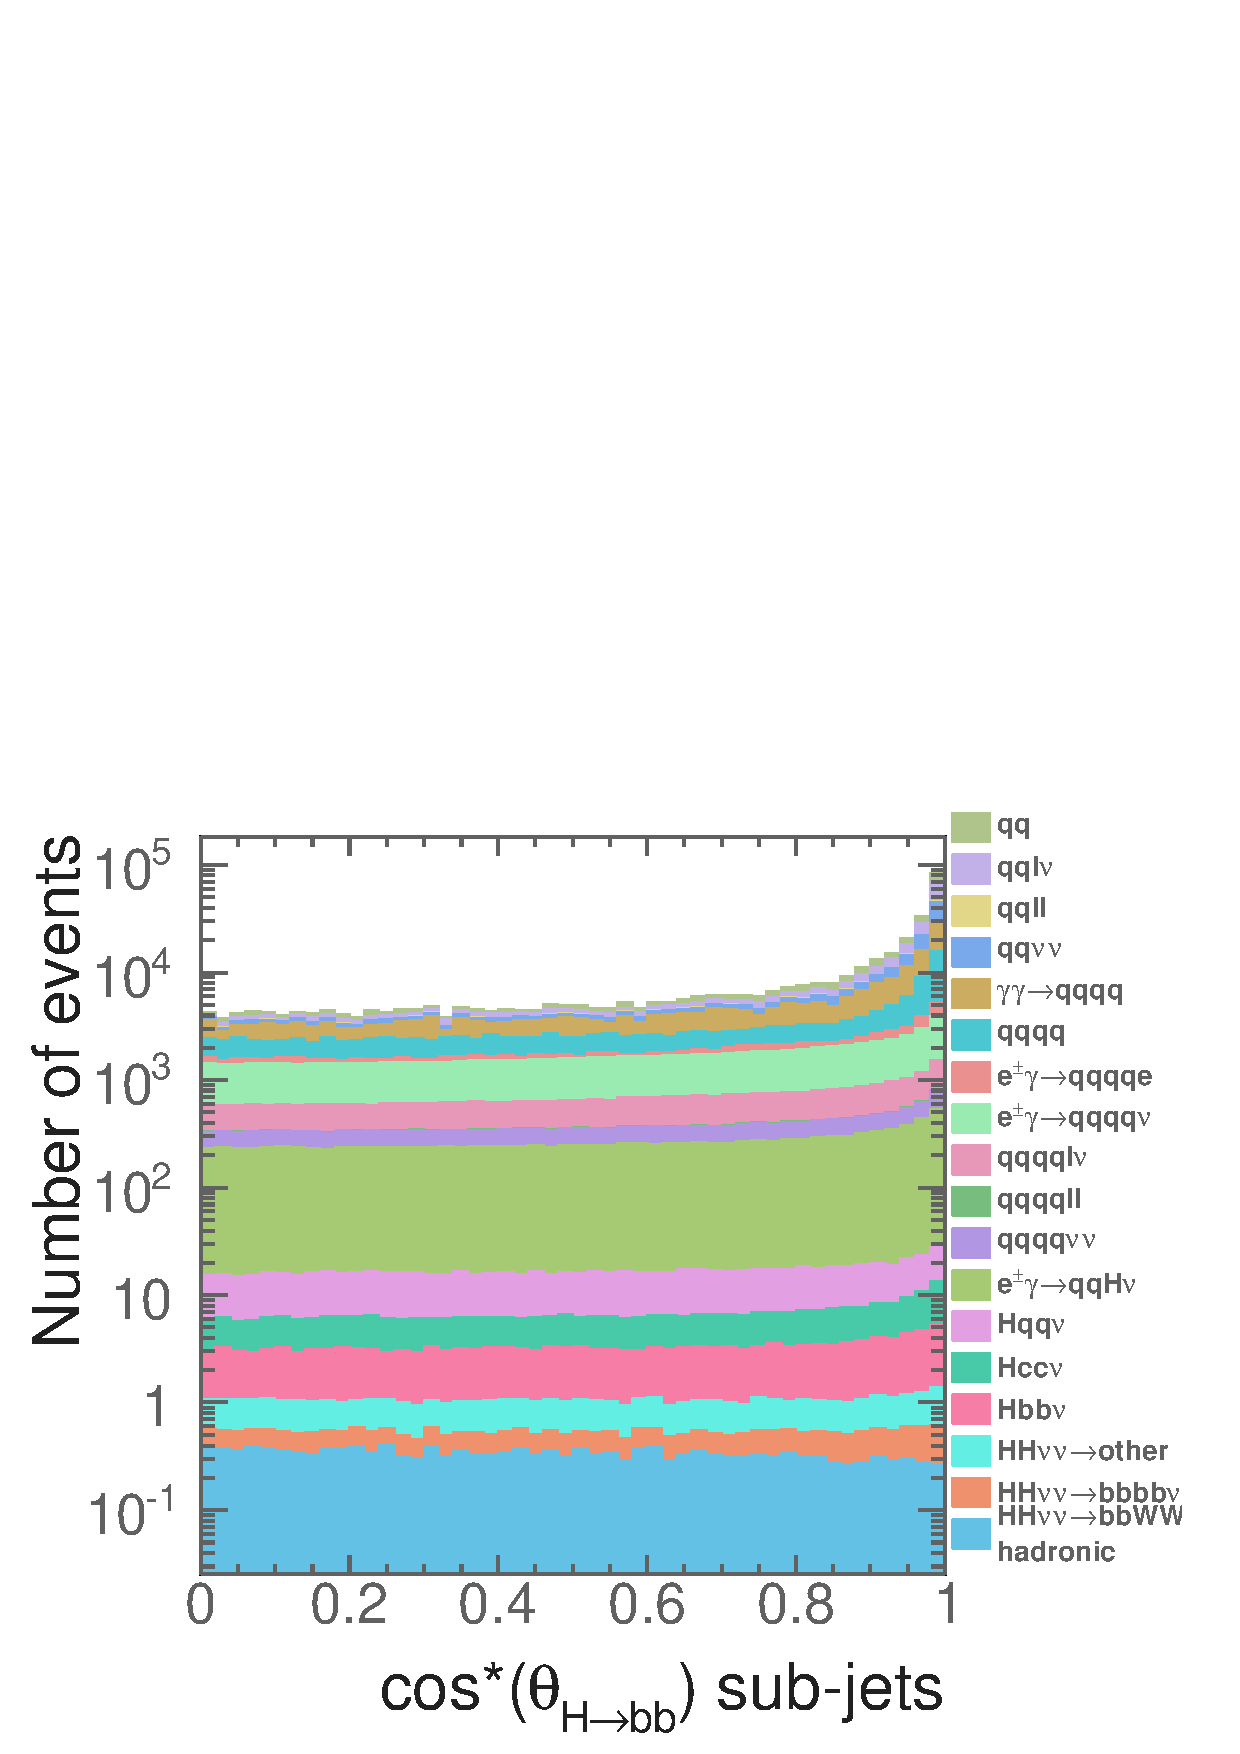
\includegraphics[width=\textwidth]{{doubleHiggs/1400var/nR0_7_6jet_btag2_Higgs1_spin_TMVA20161208R0_7_qq_btag2_prepare_testNew2}.pdf}
    \caption{}
    \label{fig:doubleHiggs1.4varSpinHbb}
  \end{subfigure}
\caption
   {Distributions of the four variables with highest discriminating power: a) the invariant mass of \Hbb, b) the invariant mas of \HWW, c) the acolinearity of the two jets associated with \Hbb, and d) the opening angles of the two jets associated with \Hbb in the decay rest frame of the \Hbb. All plots assumes an intergraded luminosity of  1500\,$fb^{-1}$ at \rootS{1.4} after all pre-selection cuts applied before the MVA.}
   \label{fig:doubleHiggs1.4var}
\end{figure}

\begin{comment}
 \begin{figure}[!tbp]
  \begin{subfigure}[b]{0.45\textwidth}
    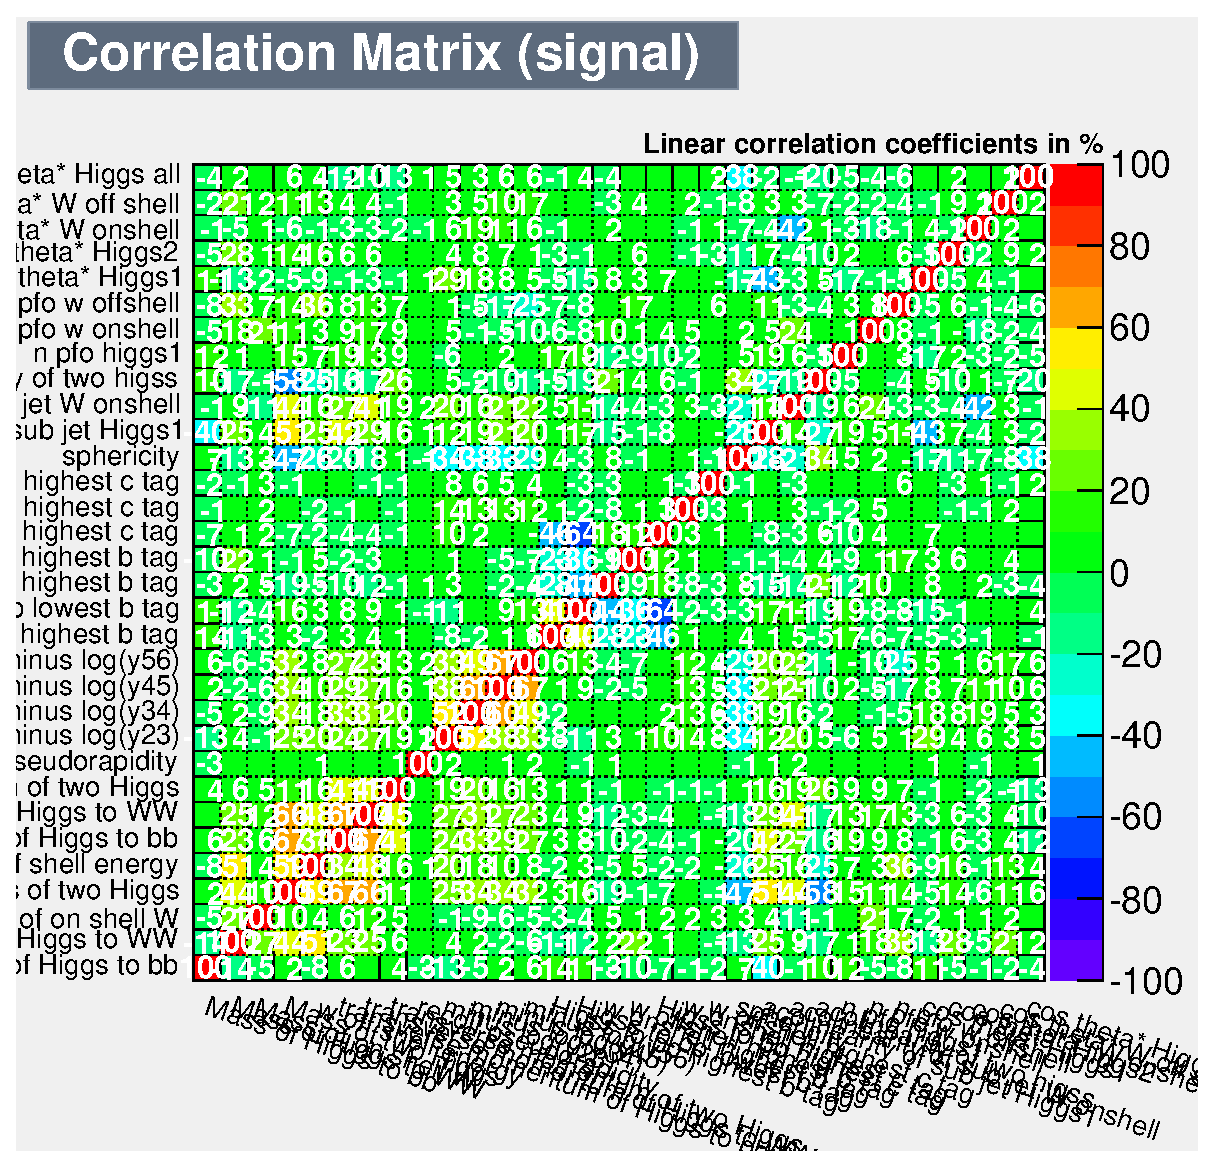
\includegraphics[width=\textwidth]{{doubleHiggs/mva/1400signalCorr}}
    \caption{}
    \label{fig:doubleHiggs1.4signalCorr}
  \end{subfigure}
    \begin{subfigure}[b]{0.45\textwidth}
    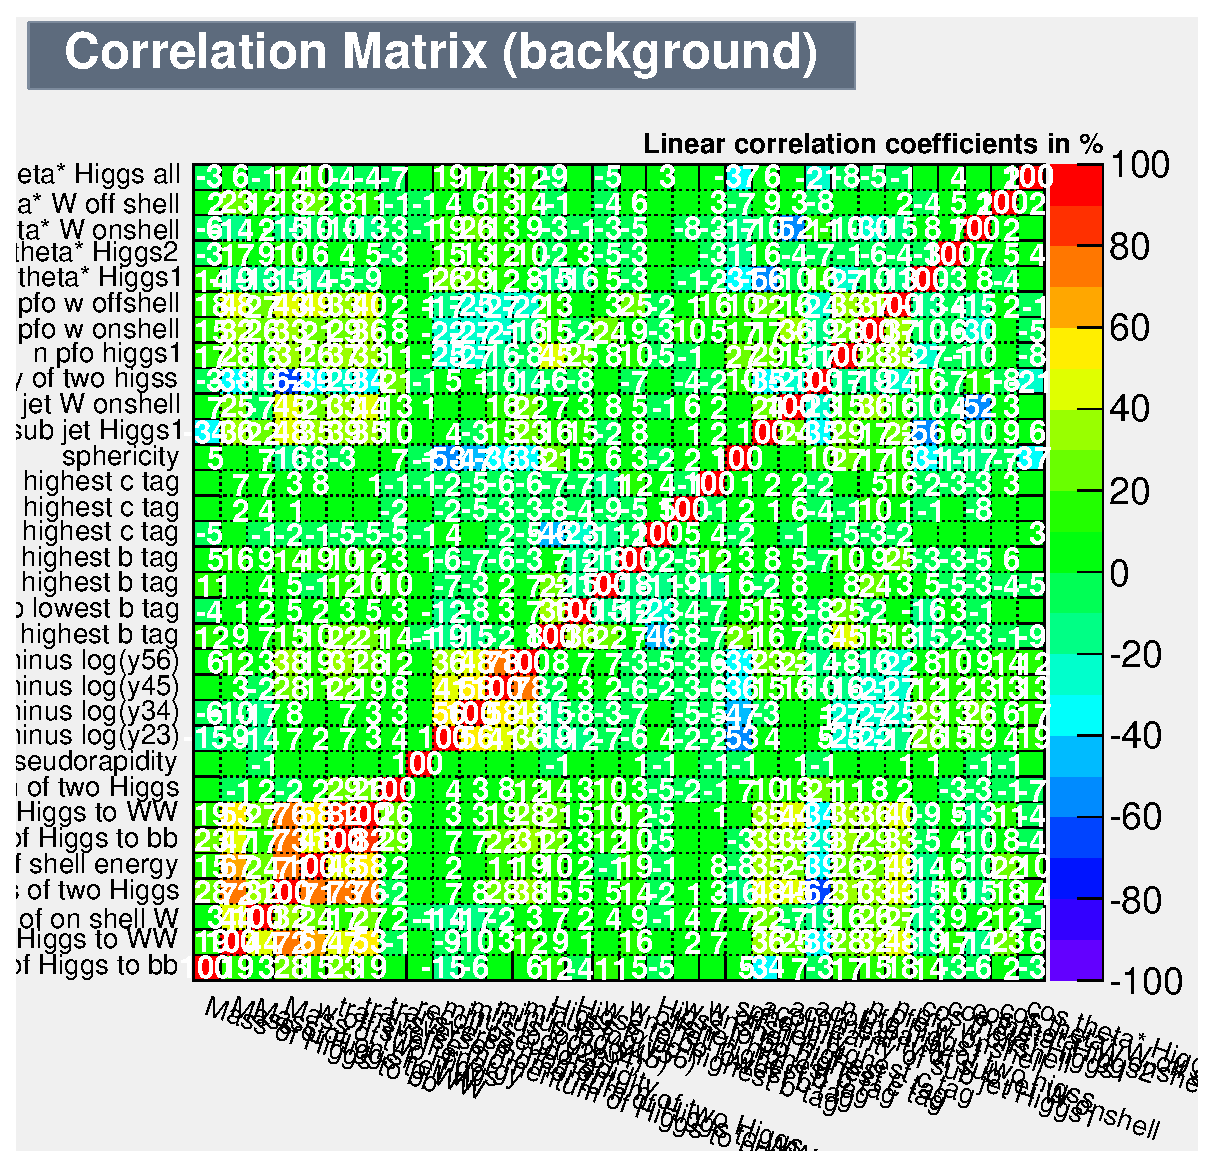
\includegraphics[width=\textwidth]{{doubleHiggs/mva/1400backgroundCorr}}
    \caption{}
    \label{fig:doubleHiggs1.4backgroundCorr}
  \end{subfigure}
\caption
   {The pair-wise correlation between discriminative variables for signal and background events at \rootS{1.4} after all pre-selection cuts.}
   \label{fig:doubleHiggs1.4Corr}
\end{figure}
\end{comment}


\subsection{Cuts to aid the MVA}

A set of cuts reduce the range of invariant masses variables in order to increase the effectiveness of the MVA event selection. (See \Section{sec:pandoraMVAbdtVar}). Occasional extreme values of the invariant masses variables skew the distributions. Therefore by limiting the range of the variables, the MVA classifier could focus on the phase spaces with high event densities. The cuts require the invariant mass of the \Hbb < 500\,GeV, the invariant mass of the \HWW < 800\,GeV, the invariant mass of the \PW < 200\,GeV, and the invariant mass of the double Higgs system < 1400\,GeV.



\section{Multivariate analysis}
\label{sec:doubleHiggsMVA}
After gathering information and applying  pre-selection cuts, signal events are selected using the multivariate analysis (MVA) with Boosted Decision Tree classifier (BDT), as implemented in the TMVA \cite{Hocker:2007ht}.. The parameters for boosted decision tree were optimised and checked for overtraining, following the strategy outlined in \Section{sec:pandoraMVA}. Half of the events were used for training, and the other half used for testing and classifier optimisation. The optimised parameters are listed in \Table{tab:doubleHiggsBDTparameters}.

After dividing all events into a training set and a testing set, in the training stage of the MVA classifier, the training signal events are the  hadronic \WW decay of the \eeToHHbbWW events in the training set. The training background events are all events without double higgs production  in the training set. However, for the extraction of the \gHHH and \gWWHH,  all events with double higgs production are sensitive to the couplings Therefore, at the applying stage of the MVA classifier, all events in the testing set are used.
%, although for example, the \eeToHHbbbb final state has a different topology to the hadronic \WW decay of the \eeToHHbbWW.


%The optimisation of the BDT follows the strategy outlined in \Section{sec:pandoraMVAbdtVar}. The optimal values are obtained by choosing the best performance without overfitting.
%at \rootS{3}. The same optimised parameters are used for \rootS{1.4} analysis.

\begin{table}[!tbp]\centering
%\small{

\begin{tabular}{lr}
\hline \hline
 Parameter &  Value \\
\hline
Depth of tree & 4 \\
Number of trees & 4000 \\
The minimum number of events in a node &  0.25\% of the total events \\
Boosting & adaptive boost \\
Learning rate of the adaptive boost & 0.5 \\
Metric for the optimal cuts & Gini Index \\
Bagging fraction & 0.5 \\
Number of bins per variables & 40 \\
End node output & x $\in [0,1]$ \\
Do-PreSelection & yes \\
\hline \hline
\end{tabular}

\caption
{Optimised parameters for the boosted decision tree classifier used in the MVA event selection. See \Section{sec:pandoraMVAbdtVar} for detailed explanations of variables.}
\label{tab:doubleHiggsBDTparameters}
\end{table}

\begin{comment}
  "!H:!V:NTrees=4000:MinNodeSize=0.25%:MaxDepth=4:BoostType=RealAdaBoost:AdaBoostBeta=0.5:UseBaggedBoost:BaggedSampleFraction=0.5:SeparationType=GiniIndex:nCuts=40:DoPreselection=True" );
\end{comment}



\section{Signal selection results}
\label{sec:doubleHiggsSignalSelResult}
%first sentence doesn't make sense. Should there be an "and" in there?

Number of events passed the MVA event selection at \rootS{1.4}, assuming a luminosity of 1500$fb^{-1}$  are listed in \Table{tab:doubleHiggs1.4TeVMVA} for individual channels. A few  background channels have non-zero events after the MVA event selection. \eeTo{\Pquark \APquark \PHiggs \Pnu \APnu} events are difficult to discard because its topology, one single Higgs plus neutrino, is very similar to the signal event topology. Similarly, \eeTo{ \Pquark \Pquark \Pquark \Pquark \Plepton \Pnu} events can be confused with the signal events when the lepton is undetected in the forward region, or the energy of the lepton is too low to be tagged. \eeTo{ \Pquark \Pquark \Pquark \Pquark \Pnu \APnu} events can also have a similar topology to the signal events. Other background channels that are not discarded after the MVA are the electron-photon and photon interactions with the same final states as the channels above.


Before interpreting the result for analysis at \rootS{1.4}, the analyses at \rootS{3} and  the semi-leptonic channel of \eeToHH $\to$ \HepProcess{ \Pbottom \APbottom \PWplus \PWminus \Pnue \APnue} are presented.





\begin{table}[!tbp]\centering
%\small{

\begin{tabular}{lrrrr}
\hline \hline
 \multicolumn{1}{m{3.5cm}}{Channel / Efficiency \rootS{1.4}} &  \multicolumn{1}{m{2cm}}{N}  & \multicolumn{1}{m{2cm}}{$\varepsilon_{presel}$} & \multicolumn{1}{m{2cm}}{$\varepsilon_{MVA}$} & \multicolumn{1}{m{2cm}}{$N_{MVA}$} \\
\hline
\eeToHH $\to$ \\
\HepProcess{ \Pbottom \APbottom \PWplus \PWminus \Pnue \APnue}, hadronic             &27.9& 59.8\% & 8.2\% & 1.29 \\
\hline
\eeToHH $\to$ \\
\HepProcess{ \Pbottom \APbottom \Pbottom \APbottom \Pnue \APnue}             &67.6& 15.4\%  & 0.5\% & 0.05\\
\eeToHH $\to$ other                             & 128.0 & 20.4\% & 1.7\% & 0.45\\
\hline
\eeTo{\qlight \qlight \PHiggs \Pnu \APnu}  & 1290 & 39.5\% & 0.05\%& 0.29\\
\eeTo{\Pcharm \APcharm \PHiggs \Pnu \APnu}  & 540 & 31.6\%& 0.1\%& 0.16\\
\eeTo{\Pbottom \APbottom \PHiggs \Pnu \APnu}  & 465 & 24.7\%& 0.3\%& 0.37\\

\eeTo{ \Pquark \Pquark \Pquark \Pquark}   &   1867650& 3.3\% & - & -\\
\eeTo{ \Pquark \Pquark \Pquark \Pquark \Plepton \Plepton}& 93150 & 0.3\%& - &  - \\
\eeTo{ \Pquark \Pquark \Pquark \Pquark \Plepton \Pnu}& 165600 & 9.8\%& 0.01\%& 2.06\\
\eeTo{ \Pquark \Pquark \Pquark \Pquark \Pnu \APnu} & 34800& 16.5\%& 0.002\% & 0.10\\

\eeTo{ \Pquark \Pquark} &  6014250 & 0.8\%& - & - \\
\eeTo{ \Pquark \Pquark \Plepton \Pnu} &  6464550 & 0.9\%&  - & - \\
\eeTo{ \Pquark \Pquark \Pl \Pl} &  4088700 & 0.08\%& - & - \\
\eeTo{ \Pquark \Pquark \Pnu \Pnu} & 1181550 & 4.0\%& - & - \\
\hline
\egamma{\Pepm}{\Pphoton}{BS}{\Pepm \Pquark \Pquark \Pquark \Pquark} & 2606625 & 0.3\%& - & -\\
%\egamma{\Pem}{\Pphoton}{BS}{\Pem \Pquark \Pquark \Pquark \Pquark} & 1305787.5  & 0.3\%& - & -\\
%\egamma{\Pep}{\Pphoton}{BS}{\Pep \Pquark \Pquark \Pquark \Pquark} & 1300837.5 & 0.4\%& -& -\\
\egamma{\Pepm}{\Pphoton}{EPA}{\Pepm \Pquark \Pquark \Pquark \Pquark} & 861000 & 0.3\%&  - &  - \\
%\egamma{\Pem}{\Pphoton}{EPA}{\Pem \Pquark \Pquark \Pquark \Pquark} & 430650.0 & 0.3\%&  - &  - \\
%\egamma{\Pep}{\Pphoton}{EPA}{\Pep \Pquark \Pquark \Pquark \Pquark}  & 430350.0 & 0.3\% & - & -\\
\egamma{\Pepm}{\Pphoton}{BS}{\Pnu \Pquark \Pquark \Pquark \Pquark}& 178987.5  & 25.7\%& 0.005\%& 2.05\\
%\egamma{\Pem}{\Pphoton}{BS}{\Pnu \Pquark \Pquark \Pquark \Pquark}& 89775.0  & 25.4\%& 0.005\%& 1.09\\
%\egamma{\Pep}{\Pphoton}{BS}{\APnu \Pquark \Pquark \Pquark \Pquark}& 89212.5 & 24.9\% & 0.004\%& 0.96\\
\egamma{\Pepm}{\Pphoton}{EPA}{\Pnu \Pquark \Pquark \Pquark \Pquark}& 52050  & 12.5\% & 0.004\% & 0.27 \\
%\egamma{\Pem}{\Pphoton}{EPA}{\Pnu \Pquark \Pquark \Pquark \Pquark}& 26100.0  & 12.6\% & - &  - \\
%\egamma{\Pep}{\Pphoton}{EPA}{\APnu \Pquark \Pquark \Pquark \Pquark}& 25950.0  & 12.4\%& 0.008\% & 0.27\\
\egamma{\Pepm}{\Pphoton}{BS}{\Pquark \Pquark \PHiggs \Pnu} & 35437.5   & 30.7\% & 0.02\% & 2.16 \\
%\egamma{\Pem}{\Pphoton}{BS}{\Pquark \Pquark \PHiggs \Pnu} & 17775   & 30.8\% & 0.02\% & 1.00 \\
%\egamma{\Pep}{\Pphoton}{BS}{\Pquark \Pquark \PHiggs \Pnu} & 17662.5  & 30.6\% & 0.02\% & 1.16 \\
\egamma{\Pepm}{\Pphoton}{EPA}{\Pquark \Pquark \PHiggs \Pnu} & 10170.0  & 16.1\% & 0.06\% & 0.95 \\
%\egamma{\Pem}{\Pphoton}{EPA}{\Pquark \Pquark \PHiggs \Pnu} & 5085  & 16.0\% & 0.04\% & 0.33 \\
%\egamma{\Pep}{\Pphoton}{EPA}{\Pquark \Pquark \PHiggs \Pnu} & 5085   & 16.2\% & 0.08\% & 0.62 \\
\hline
\gammagamma{\Pphoton}{BS}{\Pphoton}{BS}{ \Pquark \Pquark \Pquark \Pquark}& 2054951.5  & 0.2\%&  - & -\\
\gammagamma{\Pphoton}{BS}{\Pphoton}{EPA}{ \Pquark \Pquark \Pquark \Pquark}& 4521037.5  & 0.4\%& - & - \\
\gammagamma{\Pphoton}{EPA}{\Pphoton}{BS}{ \Pquark \Pquark \Pquark \Pquark}& 4539150.0 & 0.3\%&  - & - \\
\gammagamma{\Pphoton}{EPA}{\Pphoton}{EPA}{ \Pquark \Pquark \Pquark \Pquark}& 1129500.0 & 0.3\% & - & -\\
\hline \hline
\end{tabular}

\caption[Selection efficiency and number of events for signal and background at \rootS{1.4}.]%
{List of signal and background events with selection efficiency and number of events at \rootS{1.4}, assuming a luminosity of 1500$fb^{-1}$. The number of events ($N$), the selection efficiencies of pre-selection cuts ($\varepsilon_{presel}$), the selection efficiencies of MVA after pre-selection cuts ($\varepsilon_{MVA}$), and the number of events after MVA ($N_{MVA}$) are shown. - represents a number less than 0.01.}
\label{tab:doubleHiggs1.4TeVMVA}
\end{table}



\section{\rootS{3} analysis}

The the hadronic \WW decay of the \eeToHH $\to$ \HepProcess{ \Pbottom \APbottom \PWplus \PWminus \Pnu \APnu} at \rootS{3} analysis follows the same strategy as the analysis at \rootS{1.4}. Lepton finding, jet pairing and flavouring tagging have been discussed in previous sections. The differences, which have not been mentioned, will be highlighted in this section.

Cross sections of used samples are listed in \Table{tab:doubleHiggs3crossSection}. The mutually exclusive cuts to separate events into two independent sets are almost identical to the cuts used in the \rootS{1.4} analysis. \FIGURE{fig:doubleHiggs3TeVMutualPreselection} shows the sum of b-jet tag values, when the event is clustered into four jets, as a function of $-\log\parenths{\y{34}}$ for the hadronic \WW decay in \eeToHHbbWW and \eeToHHbbbb sub-channels. The optimised cuts are  $\sumBtag{4} < 2.3, \, \y{34} < 3.6$. The selection efficiencies of evens after lepton veto, the  mutually exclusive cuts  and the jet pairing for individual channel are shown in \Table{tab:doubleHiggs3TeVPreslection}.

\begin{table}[!tbp]\centering
% TODO fix lumi correction for e gamma, gamma e
% TODO change some of sample cross section for  electron-photon interaction with four quarks and a neutrino final state

%{

\begin{tabular}{lrr}
\hline \hline
Channel  &  $\sigma(\rootS{3})$ / fb   \\
\hline
\eeToHH &0.588 \\
\hline
\eeToHHbbWWFull,hadronic &0.07 \\
\eeToHHbbbbFull  &0.19 \\
\eeToHHotherFull &0.34 \\
\hline
\eeTo{\qlight \qlight \PHiggs \Pnu \APnu} & 3.06 \\
\eeTo{\Pcharm \APcharm \PHiggs \Pnu \APnu} & 1.15\\
\eeTo{\Pbottom \APbottom \PHiggs \Pnu \APnu}  & 1.78\\

\eeTo{ \Pquark \Pquark \Pquark \Pquark} & 546.5*\\
\eeTo{ \Pquark \Pquark \Pquark \Pquark \Plepton \Plepton}&169.3*\\
\eeTo{ \Pquark \Pquark \Pquark \Pquark \Plepton \Pnu} &106.6*\\
\eeTo{ \Pquark \Pquark \Pquark \Pquark \Pnu \APnu}&71.5*\\

\eeTo{ \Pquark \Pquark} &2948.9\\
\eeTo{ \Pquark \Pquark \Plepton \Pnu} &5561.1\\
\eeTo{ \Pquark \Pquark \Pl \Pl}&3319.6\\
\eeTo{ \Pquark \Pquark \Pnu \Pnu} &1317.5 \\
\hline
\egamma{\Pepm}{\Pphoton}{\BS}{\Pepm \Pquark \Pquark \Pquark \Pquark} & 2536.3*\\
%\egamma{\Pem}{\Pphoton}{BS}{\Pem \Pquark \Pquark \Pquark \Pquark} & 1268.7*\\
%\egamma{\Pep}{\Pphoton}{BS}{\Pep \Pquark \Pquark \Pquark \Pquark}  & 1267.6*\\
\egamma{\Pepm}{\Pphoton}{\EPA}{\Pepm \Pquark \Pquark \Pquark \Pquark}  & 575.7*\\
%\egamma{\Pem}{\Pphoton}{EPA}{\Pem \Pquark \Pquark \Pquark \Pquark}  & 287.9*\\
%\egamma{\Pep}{\Pphoton}{EPA}{\Pep \Pquark \Pquark \Pquark \Pquark}   & 287.8*\\
\egamma{\Pepm}{\Pphoton}{\BS}{\Pnu \Pquark \Pquark \Pquark \Pquark}  & 524.8*\\
%\egamma{\Pem}{\Pphoton}{BS}{\Pnu \Pquark \Pquark \Pquark \Pquark}  & 262.5*\\
%\egamma{\Pep}{\Pphoton}{BS}{\APnu \Pquark \Pquark \Pquark \Pquark} & 262.3*\\
\egamma{\Pepm}{\Pphoton}{\EPA}{\Pnu \Pquark \Pquark \Pquark \Pquark}  & 108.4*\\
%\egamma{\Pem}{\Pphoton}{EPA}{\Pnu \Pquark \Pquark \Pquark \Pquark}  & 54.2*\\
%\egamma{\Pep}{\Pphoton}{EPA}{\APnu \Pquark \Pquark \Pquark \Pquark}& 54.2*\\
\egamma{\Pepm}{\Pphoton}{\BS}{\Pquark \Pquark \PHiggs \Pnu}   & 117.1* \\
%\egamma{\Pem}{\Pphoton}{BS}{\Pquark \Pquark \PHiggs \Pnu}   & 58.6* \\
%\egamma{\Pep}{\Pphoton}{BS}{\Pquark \Pquark \PHiggs \Pnu}  & 58.5* \\
\egamma{\Pepm}{\Pphoton}{\EPA}{\Pquark \Pquark \PHiggs \Pnu} & 22.4* \\
%\egamma{\Pem}{\Pphoton}{EPA}{\Pquark \Pquark \PHiggs \Pnu} & 11.7* \\
%\egamma{\Pep}{\Pphoton}{EPA}{\Pquark \Pquark \PHiggs \Pnu} & 11.7* \\
\hline
\gammagamma{\Pphoton}{\BS}{\Pphoton}{\BS}{ \Pquark \Pquark \Pquark \Pquark}&13050.3*\\
\gammagamma{\Pphoton}{\BS}{\Pphoton}{\EPA}{ \Pquark \Pquark \Pquark \Pquark}&2420.6*\\
\gammagamma{\Pphoton}{\EPA}{\Pphoton}{\BS}{ \Pquark \Pquark \Pquark \Pquark}&2423.1*\\
\gammagamma{\Pphoton}{\EPA}{\Pphoton}{\EPA}{ \Pquark \Pquark \Pquark \Pquark}&402.7* \\
\hline \hline
\end{tabular}

\caption[Cross sections of samples at \rootS{3}.]
{List of signal and background samples used in the double Higgs analysis with the corresponding cross sections at \rootS{3}. \Pquark can be \Pup, \Pdown, \Pstrange, \Pbottom or \Ptop. Unless specified, \Pquark, \Plepton and \Pnu represent either particles or the corresponding anti-particles. \Pphoton(BS) represents a real photon from beamstrahlung (BS). \Pphoton(EPA) represents a ``quasi-real'' photon, simulated with the Equivalent Photon Approximation. For processes labelled with *, events are generated with the invariant mass of the total momenta of all quarks above 50\,GeV.}
\label{tab:doubleHiggs3crossSection}
\end{table}





\begin{figure}[!tbp]
  \begin{subfigure}[b]{0.45\textwidth}
    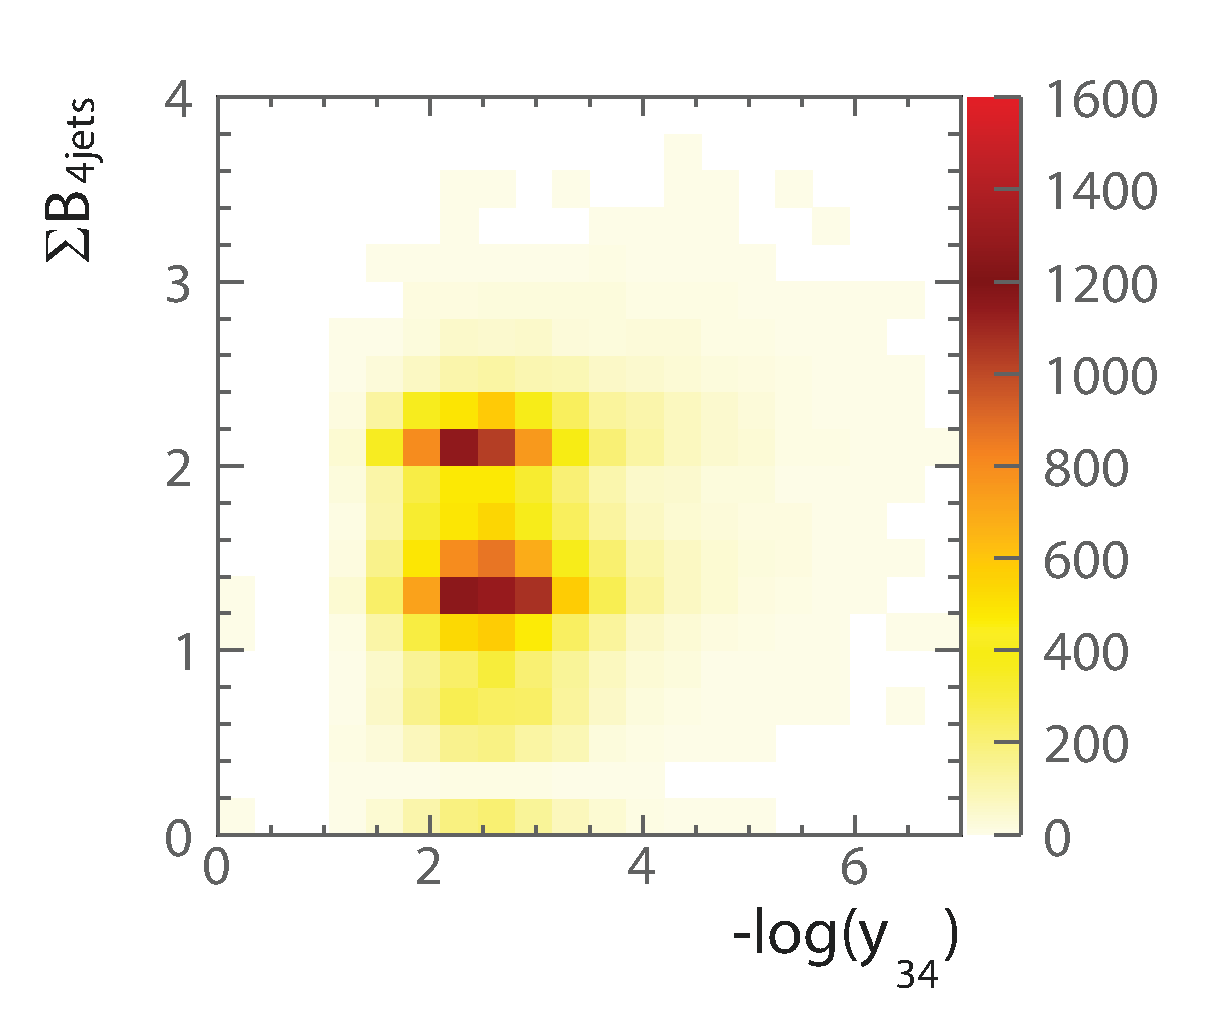
\includegraphics[width=\textwidth]{{doubleHiggs/preSel/mutual6025bbWW2}}
    \caption{\eeToHHbbWW, hadronic}
    \label{fig:doubleHiggs3MutualbbWW}
  \end{subfigure}
    \begin{subfigure}[b]{0.45\textwidth}
    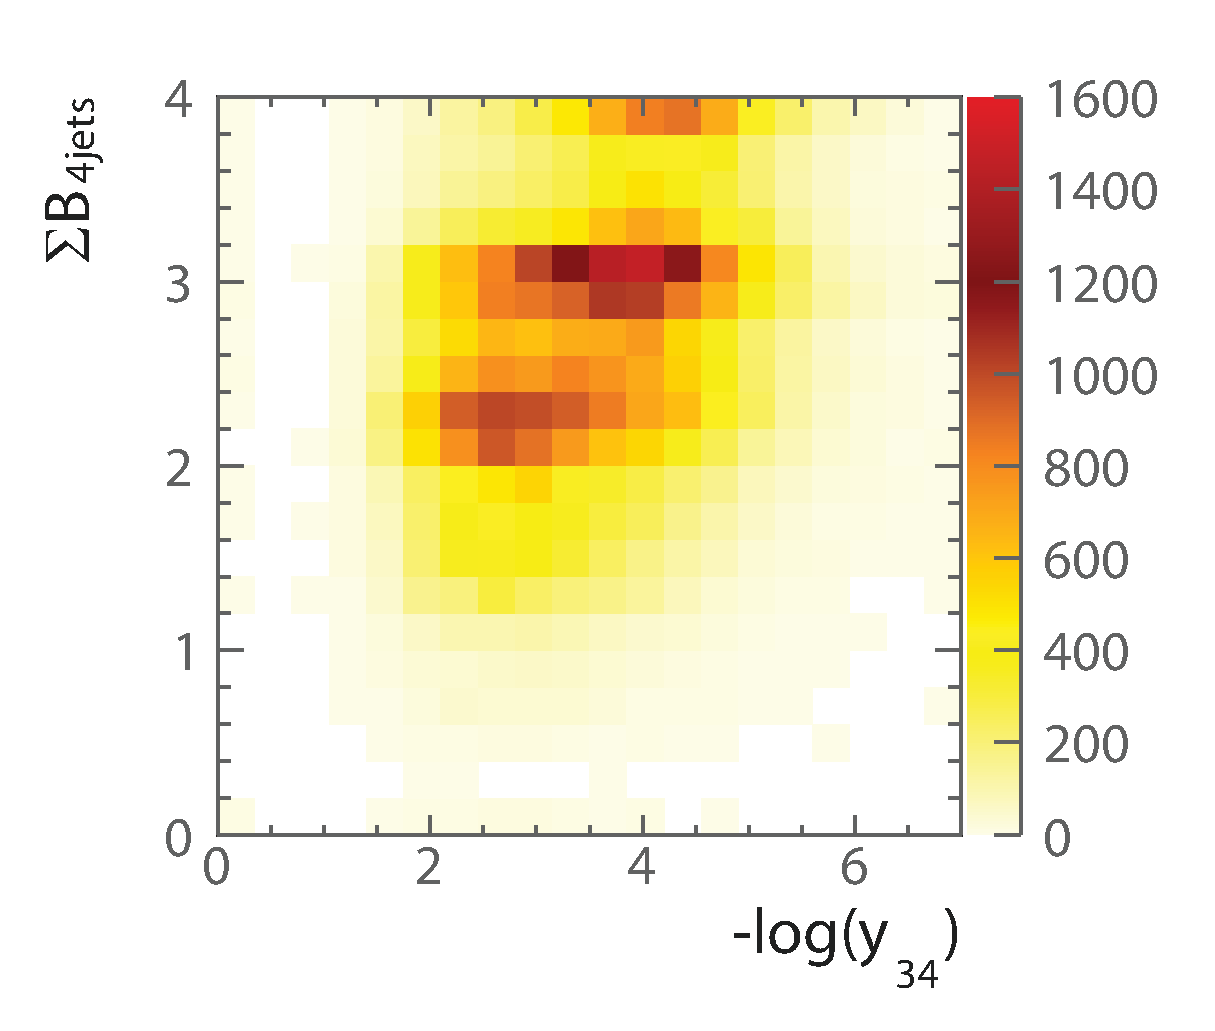
\includegraphics[width=\textwidth]{{doubleHiggs/preSel/mutual6025bbbb2}}
    \caption{\eeToHHbbbb}
    \label{fig:doubleHiggs3Mutualbbbb}
  \end{subfigure}
\caption[Sum of b-jet tag as a function of \y{34} at \rootS{3}]%
   {Sum of b-jet tag, when the event is clustered into four jets, as a function of \y{34} at \rootS{3}, shown for hadronic \WW decay of \eeToHHbbWW and \eeToHHbbbb sub-channels. }
   \label{fig:doubleHiggs3TeVMutualPreselection}
\end{figure}

The pre-selection cuts at \rootS{3} use the same cut on $m_{\HH}$. The cut on  b-jet tag is different because the performance of flavour tagging is worse at \rootS{3} in comparison to the performance at \rootS{1.4}. \FIGURE{fig:doubleHiggs3PreSelbtag} shows the distribution of the highest b-jet tag value, where the cut above 0.7 helps to reduce background events with no b-jet in final states.  \FIGURE{fig:doubleHiggs3PreSelmHH} shows the distribution of the invariant mass of the two Higgs system, where the cut above 150\,GeV is effective against samples with two-quark final states.  The fraction of events passing each pre-section cut for individual channel are listed in  \Table{tab:doubleHiggs3TeVPreslectionPart2}.


\begin{figure}[!tbp]
    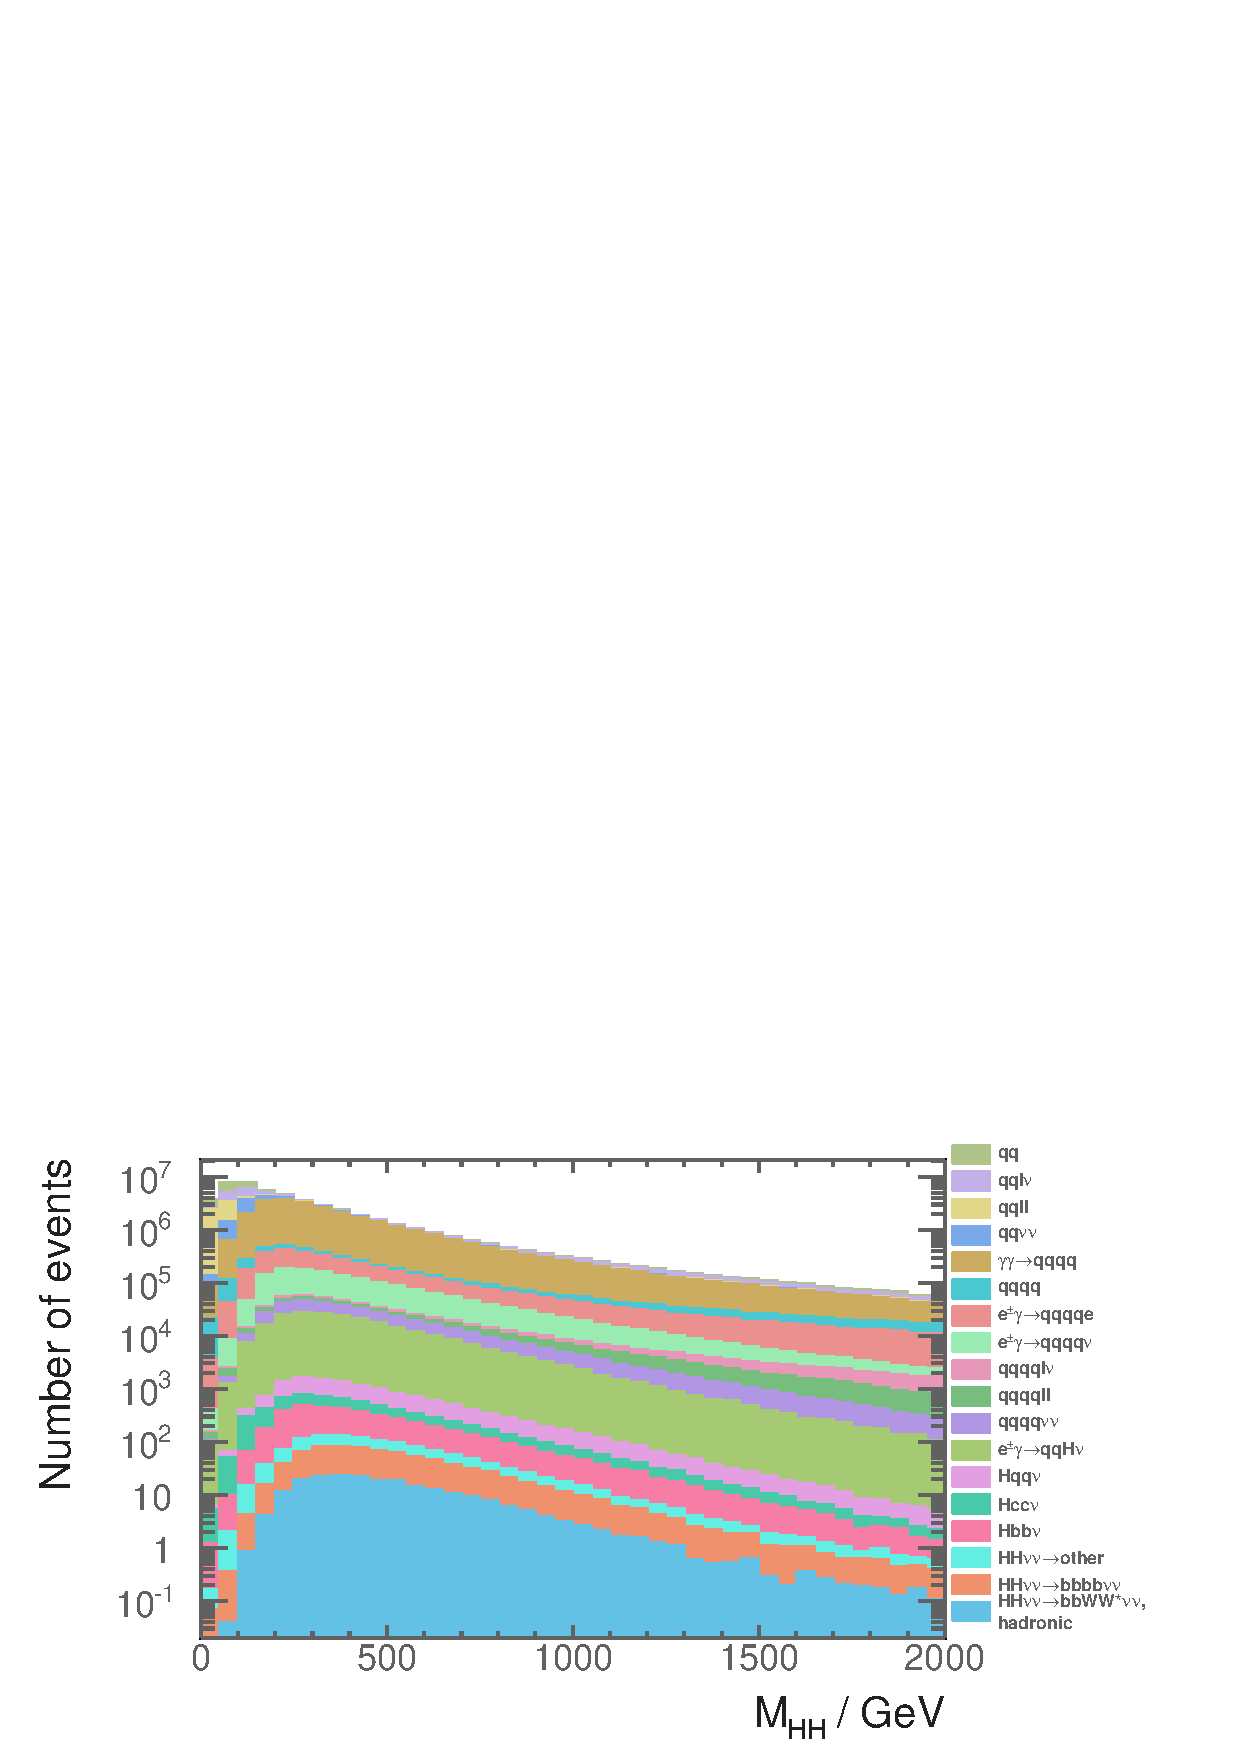
\includegraphics[width=0.85\textwidth]{{doubleHiggs/preSel/tR0_7_6jet_btag2_Higgs_all_M_TMVA201612083TeVtR0_7_qq_btag2_prepare}.pdf}
    \caption{Distributions of the invariant mass  of the two Higgs system for \rootS{3}, assuming an intergraded luminosity of 2000\,\text{$fb^{-1}$}.}
    \label{fig:doubleHiggs3PreSelmHH}
\end{figure}

\begin{figure}[!tbp]
    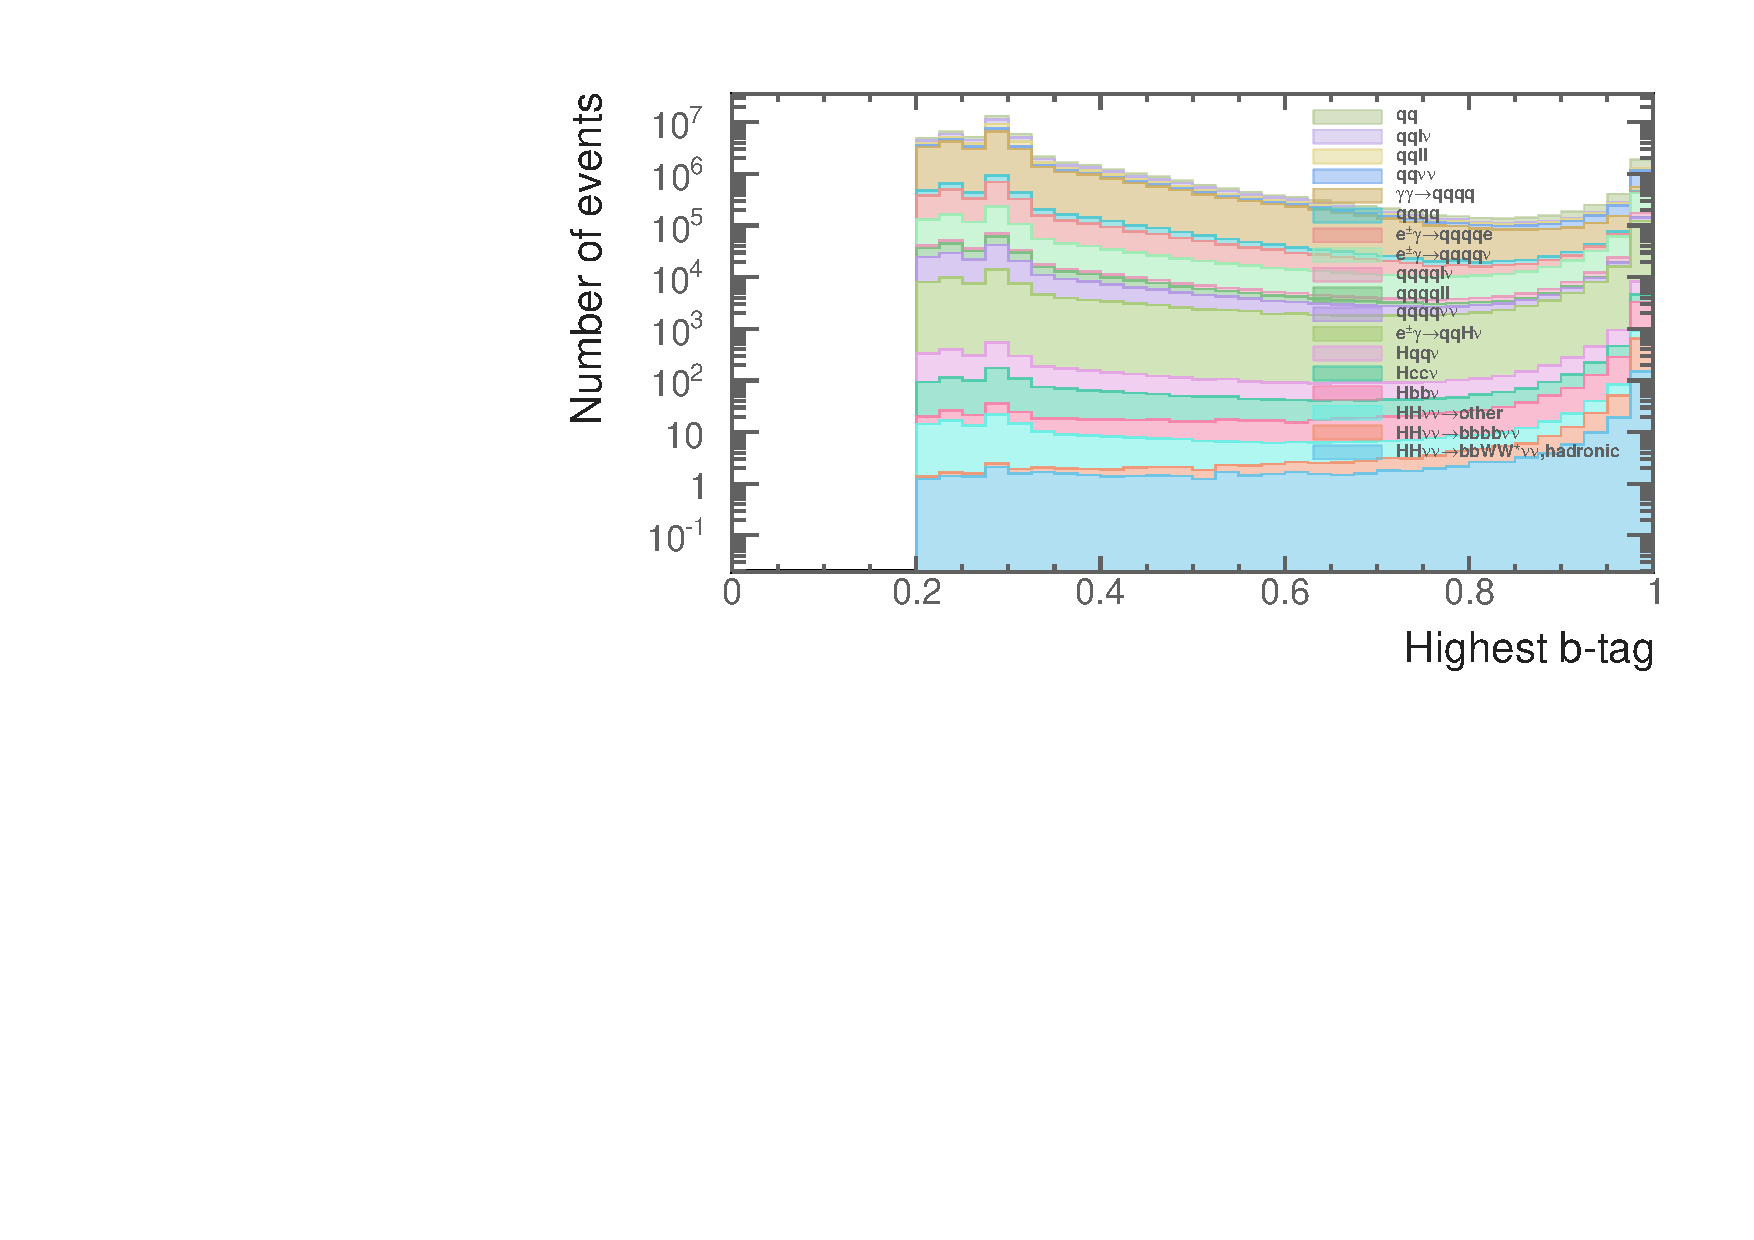
\includegraphics[width=0.85\textwidth]{{doubleHiggs/preSel/tR0_7_6jet_btag2_bTag1_TMVA201612083TeVtR0_7_qq_btag2_prepare}.pdf}
    \caption{Distributions of the highest b-jet tag value for \rootS{3}, assuming an intergraded luminosity of 2000\,\text{$fb^{-1}$}.}
    \label{fig:doubleHiggs3PreSelbtag}
\end{figure}

The cuts to aid the MVA at \rootS{3} are largely the same as the ones at \rootS{1.4}, apart from the difference on the cut of the invariant mass of \HH due to a higher \sqrtS. The cuts are  the invariant mass of the \Hbb < 500\,GeV, the invariant mass of the \HWW < 800\,GeV, the invariant mass of the \PW < 200\,GeV, and the invariant mass of the double Higgs system < 3000\,GeV.


\begin{comment}
\begin{table}[!tbp]
\begin{tabular}{lrr}
\hline
\hline
Processor / Efficiency (3\,TeV)  &  Signal  & \egamma{\Pem}{\Pphoton}{BS}{\Pem \Pquark \Pquark \Pquark \Pquark}  \\
\hline
Combined light lepton finder & 84.4\% & 72.7\%  \\
ForwardFinderProcessor & 95.9\% & 55.4\%  \\
Combined & 81.0\% &  33.4\%  \\
\hline
\hline

\end{tabular}
\caption{Very forward electron and photon finder performance on the signal and selected background samples.}
\label{tab:doubleHiggs3TeVForwardPerformance}
\end{table}
\end{comment}


% The optimal "what?" chosen is tight tightPFO?

\begin{comment}
\begin{table}[!tbp]
\begin{tabular}{lrr}
\hline
\hline
Jet Parameters  & \rootS{3}  \\
\hline
$\mu_{\Hbb}$  & $119.1_{\pm0.3}$  \\
$\sigma_{L,\Hbb}$ & $15.0_{\pm0.3}$  \\
$\sigma_{R,\Hbb}$ & $8.4_{\pm0.2}$  \\
\hline
$\mu_{\HWW}$ &  $123.0_{\pm0.3}$  \\
$\sigma_{L,\HWW}$ & $36.6_{\pm0.6}$  \\
$\sigma_{R,\HWW}$ & $7.4_{\pm0.2}$  \\
\hline
$\mu_{\PW}$  & $78.1_{\pm0.3}$ \\
$\sigma_{L,\PW}$ & $13.1_{\pm0.4}$  \\
$\sigma_{R,\PW}$ &  $9.5_{\pm0.2}$  \\
\hline
\hline
\end{tabular}
\caption
[The extracted fitted parameters of optimal jet reconstructions at \rootS{3}.] %
{The extracted fitted parameters of optimal jet reconstructions for \tightPFO with $R = 0.7$ at \rootS{3}.}
\label{tab:doubleHiggs3TeVFitParameters}
\end{table}
\end{comment}


%why have the pre-selection cuts changed?

%The cut is aggressive to compensate for the worse performance of the flavour tagging at high \sqrtS.

\begin{comment}

\begin{table}[!htbp]
\begin{tabular}{lr}
\hline
\hline
Pre-selection  &  \rootS{3}  \\
\hline
Discriminative pre-selection & \multicolumn{1}{R{0.5\textwidth}}{$m_{\HH} > 150\,GeV$, $B_1 > 0.7$,  $\pT_{\HH} > 30\,GeV$} \\
Loose cuts for MVA &  \multicolumn{1}{R{0.5\textwidth}}{$m_{\Hbb} < 500\,GeV$, $m_{\HWW} < 800\,GeV$, $m_{\PW} < 200\,GeV$, $m_{\HH} <3000\,GeV$} \\
Mutually exclusive & \sumBtag{4} < 2.3, \y{34} < 3.6 \\
\hline
\hline
\end{tabular}
\caption
{Pre-selection cuts at \rootS{3}.}
\label{tab:doubleHiggs3TeVPreSel}
\end{table}
\end{comment}
% The cut on $m_{HH}$ is effective against background with fewer number of quarks in the final states. The cut on $B_1$ is effective against final states with no b quark.





\begin{comment}
\begin{table}\centering
\begin{tabular}{llrr}
\hline
\hline
\sqrtS & $selection$ & \multicolumn{1}{m{4cm}}{\eeToHHbbqqqq Selection Efficiency} & \multicolumn{1}{m{4cm}}{\eeToHHbbbb Selection Efficiency} \\
1.4\,TeV &  \sumBtag{4} < 2.3 and \y{34} < 3.7 & 86\% & 78\% \\
3\,TeV &  \sumBtag{4} < 2.3 and \y{34} < 3.6 & 89\% & 82\% \\
\hline
\hline
\end{tabular}
\caption[Mutually exclusive cuts] %
{Mutually exclusive cuts, for full signal samples}
\label{tab:doubleHiggsMutualCuts}
\end{table}
\end{comment}

The same set of variables are used in the MVA as in the analysis at \rootS{1.4}. The optimised parameters for the Boosted Decision Tree classifier are the same. The efficiencies of the MVA event selections and the number of events after the MVA event selection are listed in \Table{tab:doubleHiggs3TeVMVA}. Background channels that are dominant after the MVA event selection are almost identical to those at \rootS{1.4}. Hence see \Section{sec:doubleHiggsSignalSelResult} for discussion.

\begin{table}[!tbp]\centering
%\small{
\small
\begin{tabular}{lrrrr}
\hline \hline
 \multicolumn{1}{m{3.5cm}}{Channel / Efficiency \rootS{3}} &  \multicolumn{1}{m{2cm}}{N}  & \multicolumn{1}{m{2cm}}{$\varepsilon_{presel}$} & \multicolumn{1}{m{2cm}}{$\varepsilon_{MVA}$} & \multicolumn{1}{m{2cm}}{$N_{MVA}$} \\

\hline
\eeToHH $\to$ \\
\HepProcess{ \Pbottom \APbottom \PWplus \PWminus \Pnue \APnue}, hadronic             &146.0& 61.7\% & 11.6\% & 9.89\\
\hline
\eeToHH $\to$ \\
\HepProcess{ \Pbottom \APbottom \Pbottom \APbottom \Pnue \APnue}             &355.0& 18.8\% & 1.5\% & 1.05 \\
\eeToHH $\to$ other                             & 675.0 & 20.0\% & 3.6\% & 4.51 \\
\hline
\eeTo{\qlight \qlight \PHiggs \Pnu \APnu}  & 6120 & 36.0\% & 0.4\% & 9.42\\
\eeTo{\Pcharm \APcharm \PHiggs \Pnu \APnu}  & 2300 & 26.3\%& 0.5\%& 3.13\\
\eeTo{\Pbottom \APbottom \PHiggs \Pnu \APnu}  & 3560 & 25.8\%& 1.2\%& 6.82\\

\eeTo{ \Pquark \Pquark \Pquark \Pquark}   &   1093000& 1.4\% & 0.01\%& 1.43\\
\eeTo{ \Pquark \Pquark \Pquark \Pquark \Plepton \Plepton}& 338600 & 0.6\%&  - & -\\
\eeTo{ \Pquark \Pquark \Pquark \Pquark \Plepton \Pnu}& 213200 & 7.3\%& 0.05\%& 8.35\\
\eeTo{ \Pquark \Pquark \Pquark \Pquark \Pnu \APnu} & 143000& 9.0\%& 0.05\%& 6.35\\

\eeTo{ \Pquark \Pquark} &  5897800 & 1.4\%&  - & - \\
\eeTo{ \Pquark \Pquark \Plepton \Pnu} &  11121800 & 0.1\%& - & - \\
\eeTo{ \Pquark \Pquark \Pl \Pl} &  6639200 & 0.4\%& - & - \\
\eeTo{ \Pquark \Pquark \Pnu \Pnu} & 2635000 & 3.1\%&  - & - \\
\hline
\egamma{\Pepm}{\Pphoton}{BS}{\Pepm \Pquark \Pquark \Pquark \Pquark} & 4007354  & 0.7\%&  - & - \\
%\egamma{\Pem}{\Pphoton}{BS}{\Pem \Pquark \Pquark \Pquark \Pquark} & 2004388.1  & 0.7\%&  - & - \\
%\egamma{\Pep}{\Pphoton}{BS}{\Pep \Pquark \Pquark \Pquark \Pquark} & 2002334.1 & 0.7\%&  - & - \\
\egamma{\Pepm}{\Pphoton}{EPA}{\Pepm \Pquark \Pquark \Pquark \Pquark} & 1151200& 0.4\%&  - & - \\
%\egamma{\Pem}{\Pphoton}{EPA}{\Pem \Pquark \Pquark \Pquark \Pquark} & 575600.0& 0.4\%&  - & - \\
%\egamma{\Pep}{\Pphoton}{EPA}{\Pep \Pquark \Pquark \Pquark \Pquark}  & 575600.0 & 0.3\% &  - & - \\
\egamma{\Pepm}{\Pphoton}{BS}{\Pnu \Pquark \Pquark \Pquark \Pquark}& 829184  & 16.4\%& 0.04\%& 61.0\\
%\egamma{\Pem}{\Pphoton}{BS}{\Pnu \Pquark \Pquark \Pquark \Pquark}& 414750.0  & 16.8\%& 0.04\%& 30.7\\
%\egamma{\Pep}{\Pphoton}{BS}{\APnu \Pquark \Pquark \Pquark \Pquark}& 414434.0 & 15.9\% & 0.05\%& 30.3\\
\egamma{\Pepm}{\Pphoton}{EPA}{\Pnu \Pquark \Pquark \Pquark \Pquark}& 216800  & 7.6\% & 0.04\%& 6.0\\
%\egamma{\Pem}{\Pphoton}{EPA}{\Pnu \Pquark \Pquark \Pquark \Pquark}& 108400.0  & 7.8\% & 0.04\%& 3.37\\
%\egamma{\Pep}{\Pphoton}{EPA}{\APnu \Pquark \Pquark \Pquark \Pquark}& 108400.0  & 7.3\%& 0.03\%& 2.63 \\
\egamma{\Pepm}{\Pphoton}{BS}{\Pquark \Pquark \PHiggs \Pnu} & 185018  & 30.2\% & 0.2\%& 121.7 \\
%\egamma{\Pem}{\Pphoton}{BS}{\Pquark \Pquark \PHiggs \Pnu} & 92588.0  & 30.2\% & 0.2\%& 67.5 \\
%\egamma{\Pep}{\Pphoton}{BS}{\Pquark \Pquark \PHiggs \Pnu} & 92430.0 & 30.3\% & 0.2\% & 54.2 \\
\egamma{\Pepm}{\Pphoton}{EPA}{\Pquark \Pquark \PHiggs \Pnu} & 46800.0 & 15.3\% & 0.2\% & 18.1 \\
%\egamma{\Pem}{\Pphoton}{EPA}{\Pquark \Pquark \PHiggs \Pnu} & 23400.0 & 15.4\% & 0.2\% & 7.88 \\
%\egamma{\Pep}{\Pphoton}{EPA}{\Pquark \Pquark \PHiggs \Pnu} & 23400.0   & 15.2\% & 0.3\% & 10.2 \\
\hline
\gammagamma{\Pphoton}{BS}{\Pphoton}{BS}{ \Pquark \Pquark \Pquark \Pquark}& 18009414  & 1.6\%&   - & - \\
\gammagamma{\Pphoton}{BS}{\Pphoton}{EPA}{ \Pquark \Pquark \Pquark \Pquark}& 3824548  & 1.0\%&  - & - \\
\gammagamma{\Pphoton}{EPA}{\Pphoton}{BS}{ \Pquark \Pquark \Pquark \Pquark}& 3828498& 1.0\%&  - & - \\
\gammagamma{\Pphoton}{EPA}{\Pphoton}{EPA}{ \Pquark \Pquark \Pquark \Pquark}& 805400 & 0.6\%&  - & - \\
\hline \hline
\end{tabular}
\caption[List of signal and background selection efficiencies and event numbers after MVA application at  \rootS{3}.]
{List of signal and background events with selection efficiency and number of events at \rootS{3}, assuming a luminosity of 2000$fb^{-1}$. The number of events ($N$), the selection efficiencies of pre-selection cuts ($\varepsilon_{presel}$), the selection efficiencies of MVA after pre-selection cuts ($\varepsilon_{MVA}$), and the number of events after MVA ($N_{MVA}$) are shown. - represents a number less than 0.01.}
\label{tab:doubleHiggs3TeVMVA}
\end{table}

\section{Semi-leptonic decay at \rootS{3} analysis}

The final analysis is the semi-leptonic \WW decay of \eeToHH $\to$ \HepProcess{ \Pbottom \APbottom \PWplus \PWminus \Pnu \APnu}  at \rootS{3}. The semi-leptonic decay analysis at \rootS{1.4} was also performed. However there are not enough signal events to have a meaningful discussion for the analysis at \rootS{1.4}. Hence, only the semi-leptonic decay analysis at \rootS{3} is presented.

The strategy of the semi-leptonic decay  analysis is very similar to the hadronic decay analysis. The main difference are that there is one lepton in the final state and the final state has four quarks instead of six. \Hbb and \PW can not be reconstructed due to the leptonic decay of one of the \PW. Hence, the signal events are selected when there is one identified lepton using the same lepton finding processors. The jet reconstruction parameters are the same as hadronic decay analysis at the \rootS{3}. There are no mutually exclusive cuts since there is no semi-leptonic analysis in the \eeToHHbbbb analysis.

The pre-selection cuts are similar to the cuts in the hadronic analysis. The invariant mass of the double Higgs system is required to be above 150\,GeV. The highest b-jet tag value is higher than 0.2. The transverse momentum of the double Higgs system is higher than 30\,GeV.

Variables used in the MVA classifier, listed in  \Table{tab:doubleHiggsVaraiblesSemiLep},  belong to  a reduced set of the variables  used in the hadronic decay analysis, as \Hbb and \PW can not be reconstructed in the semi-hadronic decay analysis. For the same reason, the cuts to aid the MVA are reduced to the invariant mass of \Hbb < 500\,GeV and the invariant mass of the double Higgs system < 3000\,GeV.



\FIGURE{tab:doubleHiggsQlv3TeVMVA} lists the  selection efficiency and number of events after the MVA event selection for individual channel at \rootS{3}, assuming a luminosity of 2000$fb^{-1}$.  Almost all background channels are non-zero after the MVA event selection. Nevertheless,  dominant background channels are almost identical to the hadronic decay analysis  at \rootS{3}. Hence discussion of the results are provided in \Section{sec:doubleHiggsSignalSelResult}.
%"dominant background channels"?
\begin{comment}
\begin{table}[!htbp]
\begin{tabular}{lr}
\hline
\hline
Pre-selection  &  \rootS{3}  \\
\hline
Discriminative pre-selection & \multicolumn{1}{R{0.5\textwidth}}{$m_{\HH} > 150\,GeV$, $B_1 > 0.2$,  $\pT_{\HH} > 30\,GeV$} \\
Loose cuts for MVA &  \multicolumn{1}{R{0.5\textwidth}}{$m_{\Hbb} < 500\,GeV$, $m_{\HH} <3000\,GeV$} \\
\hline
\hline
\end{tabular}
\caption
{Pre-selection cuts at \rootS{3} for semi-leptonic analysis.}
\label{tab:doubleHiggs3TeVPreSelSemiLep}
\end{table}
\end{comment}

 \begin{table}[!tbp]\centering
\begin{tabular}{lr}
\hline
\hline
Category &  Variable \\
\hline
Invariant mass &  \multicolumn{1}{R{0.6\textwidth}}{$m_{\Hbb}$, $m_{\PW}$, $m_{\HH}$} \\
Energy and momentum & \multicolumn{1}{R{0.6\textwidth}}{$E_{mis}$, $\pT_{\Hbb}$, $\pT_{\PW}$, $\pT_{\HH}$} \\
Lab-frame angles & \multicolumn{1}{R{0.6\textwidth}}{$\theta_{mis}$, $\acolinearity{\Hbb}$, $\acolinearity{\PW}$, $\acolinearity{\HH}$} \\
Boosted-frame frames & \multicolumn{1}{R{0.6\textwidth}}{$\cosStar{\Hbb}$, $\cosStar{\HH}$} \\
Event shape & \multicolumn{1}{R{0.6\textwidth}}{$\abs{\sphericity}$, $-\ln(\y{23})$, $-\ln(\y{34})$, $-\ln(\y{45})$, $-\ln(\y{56})$} \\
\Pbottom and \Pcharm tag & \multicolumn{1}{R{0.6\textwidth}}{$\btagFull{1,\Hbb}$, $\btagFull{2,\Hbb}$, $\btagFull{1,\PW}$, $\ctagFull{1,\Hbb}$, $\ctagFull{1,\PW}$} \\
\PFOs number &  \multicolumn{1}{R{0.6\textwidth}}{$\npfo{\Hbb}$, $\npfo{\PW}$} \\
\hline
\hline
\end{tabular}
\caption
{Variables used in the MVA event selection for the semi-leptonic \WW decay of \eeToHHbbWW analysis  at \rootS{3}.}
\label{tab:doubleHiggsVaraiblesSemiLep}
\end{table}





\begin{table}[!tbp]\centering
%\small{

\begin{tabular}{lrrrr}
\hline \hline
 \multicolumn{1}{m{3.5cm}}{Channel / Efficiency \rootS{1.4}} &  \multicolumn{1}{m{2cm}}{N}  & \multicolumn{1}{m{2cm}}{$\varepsilon_{presel}$} & \multicolumn{1}{m{2cm}}{$\varepsilon_{MVA}$} & \multicolumn{1}{m{2cm}}{$N_{MVA}$} \\
\hline
\eeToHH $\to$ \\
\HepProcess{ \Pbottom \APbottom \PWplus \PWminus \Pnue \APnue}, semi-leptonic       &96.8& 44.6\% & 21.9\% & 13.11\\
\hline
\eeToHH $\to$ \\
\HepProcess{ \Pbottom \APbottom \Pbottom \APbottom \Pnue \APnue}             &355.0& 13.3\% & 10.9\% &  5.38\\
\eeToHH $\to$ other                             & 724.2 & 13.1\% & 13.6\% &  12.75\\
\hline
\eeTo{\qlight \qlight \PHiggs \Pnu \APnu}  & 6120 & 7.4\% & 13.7\% & 62.63\\
\eeTo{\Pcharm \APcharm \PHiggs \Pnu \APnu}  & 2300 & 6.3\%& 12.1\%& 17.10\\
\eeTo{\Pbottom \APbottom \PHiggs \Pnu \APnu}  & 3560 & 15.9\%& 5.1\%& 18.03\\

\eeTo{ \Pquark \Pquark \Pquark \Pquark}   &   1093000& 0.6\% & 0.2\%& 15.04\\
\eeTo{ \Pquark \Pquark \Pquark \Pquark \Plepton \Plepton}& 338600 & 1.0\%&  0.06\% & 1.85\\
\eeTo{ \Pquark \Pquark \Pquark \Pquark \Plepton \Pnu}& 213200 & 27.6\%& 0.5\%& 270.33\\
\eeTo{ \Pquark \Pquark \Pquark \Pquark \Pnu \APnu} & 143000& 1.9\%& 1.6\%& 43.78\\

\eeTo{ \Pquark \Pquark} &  5897800 & 0.4\%&  0.3\% & 60.82 \\
\eeTo{ \Pquark \Pquark \Plepton \Pnu} &  11121800 & 0.3\%& 0.08\% & 21.24 \\
\eeTo{ \Pquark \Pquark \Pl \Pl} &  6639200 & 0.6\%& 0.2\%& 84.14\\
\eeTo{ \Pquark \Pquark \Pnu \Pnu} & 2635000 & 0.4\%&  0.9\% & 92.55 \\
\hline
\egamma{\Pepm}{\Pphoton}{\BS}{\Pepm \Pquark \Pquark \Pquark \Pquark} & 4007354  & 1.2\%&  - & - \\
%\egamma{\Pem}{\Pphoton}{BS}{\Pem \Pquark \Pquark \Pquark \Pquark} & 2004388.1  & 1.2\%&  - & - \\
%\egamma{\Pep}{\Pphoton}{BS}{\Pep \Pquark \Pquark \Pquark \Pquark} & 2002334.1 & 1.2\%&  - & - \\
\egamma{\Pepm}{\Pphoton}{\EPA}{\Pepm \Pquark \Pquark \Pquark \Pquark} & 1151200& 1.1\%&  - & - \\
%\egamma{\Pem}{\Pphoton}{EPA}{\Pem \Pquark \Pquark \Pquark \Pquark} & 575600.0& 1.1\%&  - & - \\
%\egamma{\Pep}{\Pphoton}{EPA}{\Pep \Pquark \Pquark \Pquark \Pquark}  & 575600.0 & 1.1\% &  - & - \\
\egamma{\Pepm}{\Pphoton}{\BS}{\Pnu \Pquark \Pquark \Pquark \Pquark}& 829184  & 3.6\%& 1.5\%& 452.45\\
%\egamma{\Pem}{\Pphoton}{BS}{\Pnu \Pquark \Pquark \Pquark \Pquark}& 414750.0  & 3.7\%& 1.5\%& 226.77\\
%\egamma{\Pep}{\Pphoton}{BS}{\APnu \Pquark \Pquark \Pquark \Pquark}& 414434.0 & 3.5\% & 1.6\%& 225.68\\
\egamma{\Pepm}{\Pphoton}{\EPA}{\Pnu \Pquark \Pquark \Pquark \Pquark}& 216800  & 11.0\% & 0.9\%& 200.65\\
%\egamma{\Pem}{\Pphoton}{EPA}{\Pnu \Pquark \Pquark \Pquark \Pquark}& 108400.0  & 11.2\% & 0.9\%& 107.90\\
%\egamma{\Pep}{\Pphoton}{EPA}{\APnu \Pquark \Pquark \Pquark \Pquark}& 108400.0  & 10.7\%& 0.8\%& 92.75 \\
\egamma{\Pepm}{\Pphoton}{\BS}{\Pquark \Pquark \PHiggs \Pnu} & 185018  & 7.9\% & 10.4\%& 1521.93 \\
%\egamma{\Pem}{\Pphoton}{BS}{\Pquark \Pquark \PHiggs \Pnu} & 92588.0  & 7.9\% & 10.7\%& 779.36 \\
%\egamma{\Pep}{\Pphoton}{BS}{\Pquark \Pquark \PHiggs \Pnu} & 92430.0 & 7.9\% & 10.1\% & 741.57 \\
\egamma{\Pem}{\Pphoton}{\EPA}{\Pquark \Pquark \PHiggs \Pnu} & 46800 & 22.8\% & 7.1\% & 750.85 \\
%\egamma{\Pem}{\Pphoton}{EPA}{\Pquark \Pquark \PHiggs \Pnu} & 23400.0 & 22.9\% & 6.9\% & 369.52 \\
%\egamma{\Pep}{\Pphoton}{EPA}{\Pquark \Pquark \PHiggs \Pnu} & 23400.0   & 22.7\% & 7.2\% & 381.33 \\
\hline
\gammagamma{\Pphoton}{\BS}{\Pphoton}{\BS}{ \Pquark \Pquark \Pquark \Pquark}& 18009414  & 0.4\%&   - & - \\
\gammagamma{\Pphoton}{\BS}{\Pphoton}{\EPA}{ \Pquark \Pquark \Pquark \Pquark}& 3824548 & 1.0\%&  - & - \\
\gammagamma{\Pphoton}{\EPA}{\Pphoton}{\BS}{ \Pquark \Pquark \Pquark \Pquark}& 3828498 & 1.0\%&  0.08\% & 28.85 \\
\gammagamma{\Pphoton}{\EPA}{\Pphoton}{\EPA}{ \Pquark \Pquark \Pquark \Pquark}& 805400& 1.1\%&  - & - \\
\hline \hline
\end{tabular} semi-leptonic \WW decay of \eeToHHbbWW
\caption
{List of signal and background events with selection efficiency and number of events at \rootS{3}  for semi-leptonic \WW decay of \eeToHHbbWW analysis , assuming a luminosity of 2000$fb^{-1}$. The number of events ($N$), the selection efficiencies of pre-selection cuts ($\varepsilon_{presel}$), the selection efficiencies of MVA after pre-selection cuts ($\varepsilon_{MVA}$), and the number of events after MVA ($N_{MVA}$) are shown. - represents a number less than 0.01}
\label{tab:doubleHiggsQlv3TeVMVA}
\end{table}

\section{Result interpretation}
\label{sec:doubleHiggsResults}



The results of analyses at the \rootS{1.4} and \rootS{3}  are summarised in \Table{tab:doubleHiggsResult}. For the hadronic \WW decay of \eeToHHbbWW analyses at \rootS{1.4} and \rootS{3}, numbers of the signal events passing the MVA event selection are 1.79 and 15.45, respectively; the numbers of background events passing the MVA event selection are 8.41 and 242.28, respectively. For  the semi-leptonic \WW decay of \eeToHHbbWW analyses \rootS{3}, the number of the signal events passing the MVA event selection is 31.24, whilst the  numbers of background events passing the MVA event selection is 3612.39.



The expected uncertainty on the measurement of the cross sections, which is roughly $\sqrt{N_S + N_B} / N_S$ at \rootS{1.4} and 3\,TeV, are:
\begin{equation}
\frac{\Delta\left[\sigma\left(\HHvv\right)\right]}{\sigma\left(\HHvv\right)}=
\begin{cases}
  179\%, & \mbox{at \rootS{1.4}, }  \\
  92\%, & \mbox{at \rootS{3}},
\end{cases}
\end{equation}
where $N_S$ is the number of  \eeToHH events passing the MVA event selection and $N_B$ is the number of background events passing the MVA event selection. The result at \rootS{3} combines both the hadronic and semi-leptonic decay sub-channels.

\begin{table}[!htbp]
\begin{tabular}{lrrr}
\hline
\hline
Channel  &  $N_{S}$ & $N_{B}$ & $N_S / \sqrt{N_S + N_B}$ \\
\hline
\multicolumn{1}{L{0.3\textwidth}}{\eeToHHbbWW, hadronic, \rootS{1.4}} & 1.79 & 8.41 & 0.56 \\
\multicolumn{1}{L{0.3\textwidth}}{\eeToHHbbWW, hadronic, \rootS{3}} & 15.45 & 242.28 & 0.96 \\
\multicolumn{1}{L{0.3\textwidth}}{\eeToHHbbWW, semi-leptonic, \rootS{3}} &  31.24& 3612.39 & 0.52 \\
\hline
\hline
\end{tabular}
\caption
{Number of signal and background events, and significance after MVA for all \eeToHHbbWW analyses.}
\label{tab:doubleHiggsResult}
\end{table}


As previously stated, the double Higgs production cross section is sensitive to the Higgs trilinear self coupling \gHHH. The relative uncertainty on the coupling can be related to the uncertainty on the coupling via:
\begin{equation}
\frac{\Delta\gHHH}{\gHHH}\approx \kappa \cdot \frac{\Delta\left[\sigma\left(\HHvv\right)\right]}{\sigma\left(\HHvv\right)},
\label{eqn:doubleHiggs1Dextration}
\end{equation}
$\kappa$ can be extracted by varying the \gHHH and parameterising the cross section change at a general level. \FIGURE{fig:doubleHiggsCouplingOneDRelation} shows the cross sections as a function of the coupling at generator level for \rootS{1.4} and \rootS{3}  \cite{Abramowicz:2016zbo}. The negative gradient indicates that the Feynman diagram sensitive to the \gHHH experiences destructive interferences with other SM Feynman  diagrams. At the SM \gHHH value, the $\kappa$ is 1.22 and 1.47 at \rootS{1.4} and 3\,TeV respectively.
%Since $\kappa$ is extracted from the relation at generator level, the fully simulated reconstruction selection may favour certain Feynman diagrams, therefore affecting the sensitivity to $\lambda$ .
\begin{figure}[!tbp]
    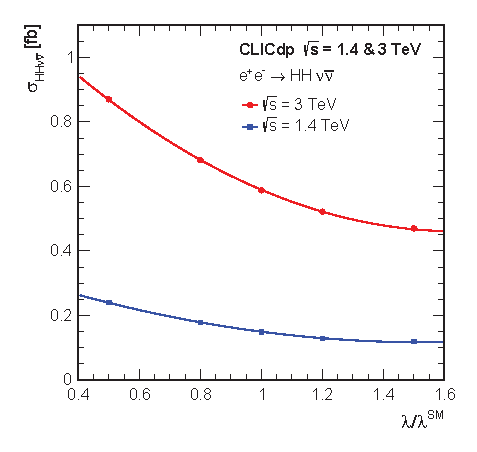
\includegraphics[width=0.45\textwidth]{{doubleHiggs/extraction/oneDrelation}}
\caption[Cross section for the \eeToHH process as a function of the ratio $\lambda/\lambda_{SM}$ ]
{Cross section for the \eeToHH process as a function of the ratio $\lambda/\lambda_{SM}$ at \rootS{1.4} and 3\,TeV, taken from \cite{Abramowicz:2016zbo}. Here $\lambda$ is the Higgs trilinear self coupling, \gHHH.}
   \label{fig:doubleHiggsCouplingOneDRelation}
\end{figure}

%Without electron polarisation,
The uncertainty on measurement of the Higgs trilinear self coupling $\lambda$, from  \eeToHH $\to$ \HepProcess{ \Pbottom \APbottom \PWplus \PWminus \Pnue \APnue} analysis is obtained via \Equation{eqn:doubleHiggs1Dextration}:
\begin{equation}
\frac{\Delta\gHHH}{\gHHH}=
\begin{cases}
  218\%, & \mbox{at \rootS{1.4}, }  \\
  135\%, & \mbox{at \rootS{3}}.
\end{cases}
\end{equation}

Since the Feynman diagrams for the double Higgs boson productions include t-channel $\HepProcess{\PW\PW}$-fusion, the cross section can be enhanced by using polarised electron beam. For $P(\Pem) = 80\%$, the uncertainty of \gHHH via \Equation{eqn:doubleHiggs1Dextration} becomes:
\begin{equation}
\frac{\Delta\gHHH}{\gHHH}=
\begin{cases}
  163\%, & \mbox{at \rootS{1.4}, }  \\
  97\%, & \mbox{at \rootS{3}}.
\end{cases}
\end{equation}
When both \sqrtS are combined, the statistical precision on \lambda increases to 99\% for the unpolarised beam, and 87\% for the polarised beam with  $P(\Pem) = 80\%$.

\section{Combined results}

When \eeToHHbbWW and \eeToHHbbbb sub-channels are combined, the expected precisions on the cross sections are:
\begin{equation}
\frac{\Delta\left[\sigma\left(\HHvv\right)\right]}{\sigma\left(\HHvv\right)}=
\begin{cases}
  44\%, & \mbox{at \rootS{1.4}, }  \\
  20\%, & \mbox{at \rootS{3}},
\end{cases}
\end{equation}

This translates to the uncertainty on the Higgs trilinear self coupling \gHHH, via \Equation{eqn:doubleHiggs1Dextration}, without electron polarisation:
\begin{equation}
\frac{\Delta\gHHH}{\gHHH}=
\begin{cases}
  54\%, & \mbox{at \rootS{1.4}, }  \\
  29\%, & \mbox{at \rootS{3}}.
\end{cases}
\end{equation}

\section{Simultaneous couplings extraction}

As stated in the beginning of the chapter the study of the double Higgs production via \WW fusion can probe the Higgs trilinear self coupling, \gHHH and quartic coupling, \gWWHH. Therefore, a simultaneous extraction on the coupling uncertainty can be performed by extending the method in the previous sections. Once a relationship between \gHHH , \gWWHH and difference in kinematic variable distributions is established, a contour of the uncertainty in \gHHH and \gWWHH two dimensional phase space can be obtained.

This two dimensional template fitting is performed at  \rootS{3}, as the precision at \rootS{1.4} is too low to support such a fitting. The integrated luminosity is assumed to be 3000$fb^{-1}$ to reflect the updated \CLIC running scenario.

The normalised cross section of the \eeToHH as a function of \gHHH and \gWWHH is shown in \Figure{fig:doubleHiggsCouplingCrossSection}. The SM cross section is normalised to 1. Around the SM coupling value, the cross section increases with the decrease of \gHHH and with the increase of \gWWHH. Hence the cross sections along the anti-diagonal are nearly constant, which would be difficult to precisely determine the statistical uncertainty on the coupling measurements.

\begin{figure}[!tbp]
    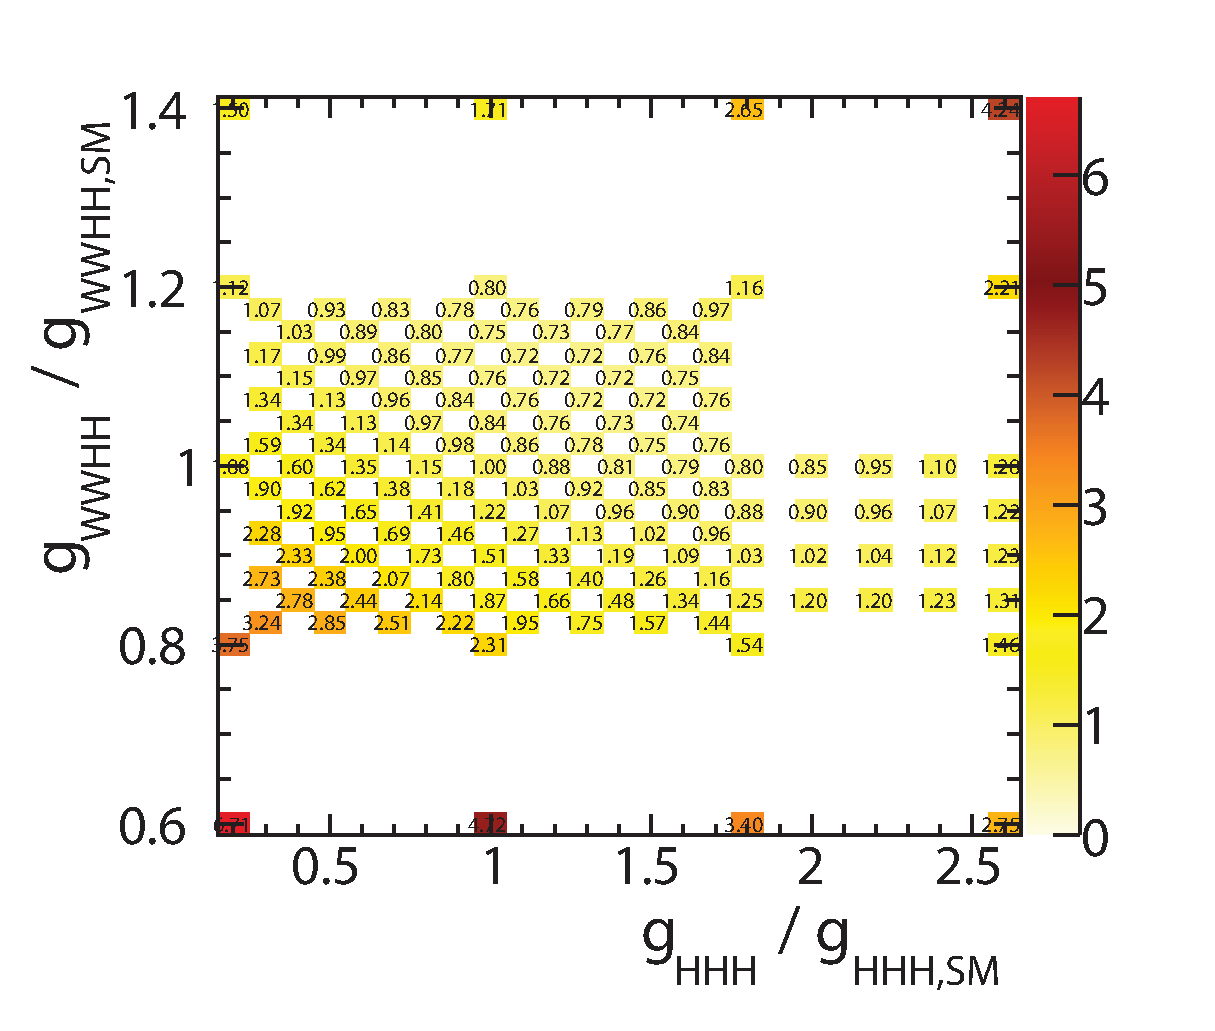
\includegraphics[width=0.85\textwidth]{{doubleHiggs/extraction/crossSectionNew2}}
\caption{Normalised cross section for the \eeToHH process as a function of the $\gHHH/\gHHH_{SM}$ and  $\gWWHH/\gWWHH_{SM}$ at \rootS{3}.}
   \label{fig:doubleHiggsCouplingCrossSection}
\end{figure}

To determine the uncertainty on the coupling measurements, the variables proposed in the generator-level study in \Section{sec:theoryHiggsBSM} are used: the invariant mass of the two Higgs system, \mhh, and the scalar sum of the two Higgs transverse momentum, \HT.  %By choosing kinematic bins, high-energy behaviour can be disentailed from the physics at threshold, allowing the extraction of the coupling strength \gWWHH and \gHHH.

Simulated events with non-SM couplings are generated and reconstructed. These events went through the analysis chain discussed in this chapter with the same cuts and the same MVA classifier.  \FIGURE{fig:doubleHiggsCouplingSignificancebbWW} shows the  signal significance of the double Higgs events with hadronic \WW decay of \eeToHHbbWW sub-channel as a function of  \gHHH and \gWWHH.

\begin{figure}[!tbp]
    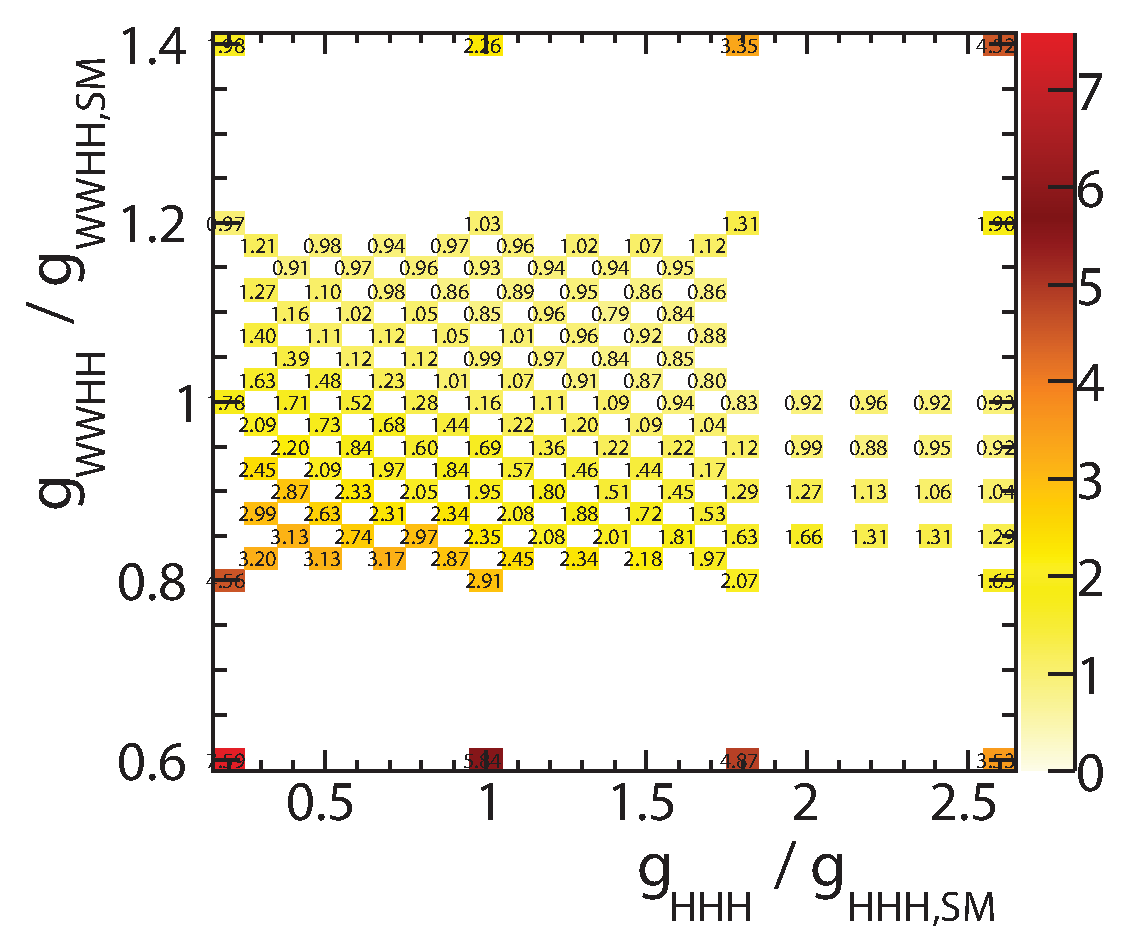
\includegraphics[width=0.8\textwidth]{doubleHiggs/extraction/SignificanceBono3}
\caption{The significance for the \eeToHH process as a function of the $\gHHH/\gHHH_{SM}$ and  $\gWWHH/\gWWHH_{SM}$ at \rootS{3}, using sub-channel hadronic \WW decay of \eeToHHbbWW, assuming an integrated luminosity of  3000$fb^{-1}$.}
   \label{fig:doubleHiggsCouplingSignificancebbWW}
\end{figure}

The selected events are divided into 8 kinematic bins. Two bins in \HT are obtained by dividing the \HT distribution at 200\,GeV. Four bins in \mhh are obtained by dividing the \mhh distribution at 400, 560, and 720\,GeV. A $\chi^2$ function is constructed to access the difference of the \mhh and \HT distributions for  non-SM coupling comparing to SM coupling sample, defined as:
\begin{equation}
\chi^2 = \sum_{i}^{bins}\frac{\parenths{N_i - N_{i,observed}}^2}{N_{i}},
\end{equation}
where $N_i$ is the number of event expected in a kinematic bin $i$ for a non-SM coupling sample. $ N_{i,observed}$ is the number of event observed in a kinematic bin $i$. Here the observed set is the SM coupling sample. The expression is summing over all kinematic bins. By construction, the SM coupling point has a $\chi^2$ of 0. \FIGURE{fig:doubleHiggsCouplingChi2Separate} shows the $\chi^2$  as a function of \gHHH and \gWWHH for two sub-channels; hadronic \WW decay of \eeToHHbbWW and \eeToHHbbbb. The $\chi^2$ values for the \eeToHHbbbb sub-channel are larger as the \eeToHHbbbb is more sensitive to the couplings.

\begin{figure}[!tbp]
  \begin{subfigure}[b]{0.45\textwidth}
    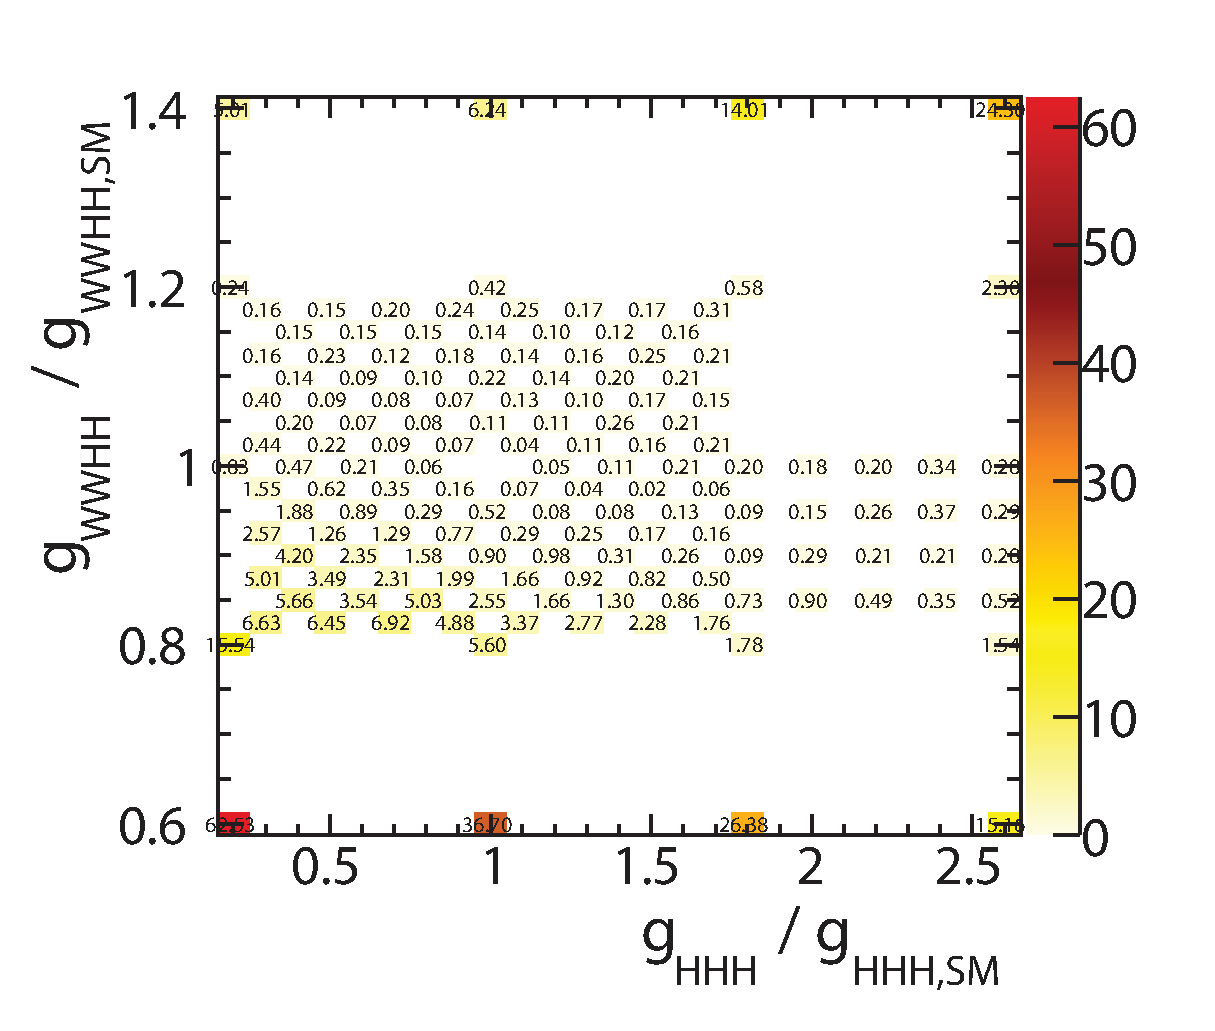
\includegraphics[width=\textwidth]{{doubleHiggs/extraction/new/chi2Bono4mhh2HT2}}
    \caption{\eeToHHbbWWHad, hadronic}
    \label{fig:doubleHiggsCouplingChi2bbWW}
  \end{subfigure}
    \begin{subfigure}[b]{0.45\textwidth}
    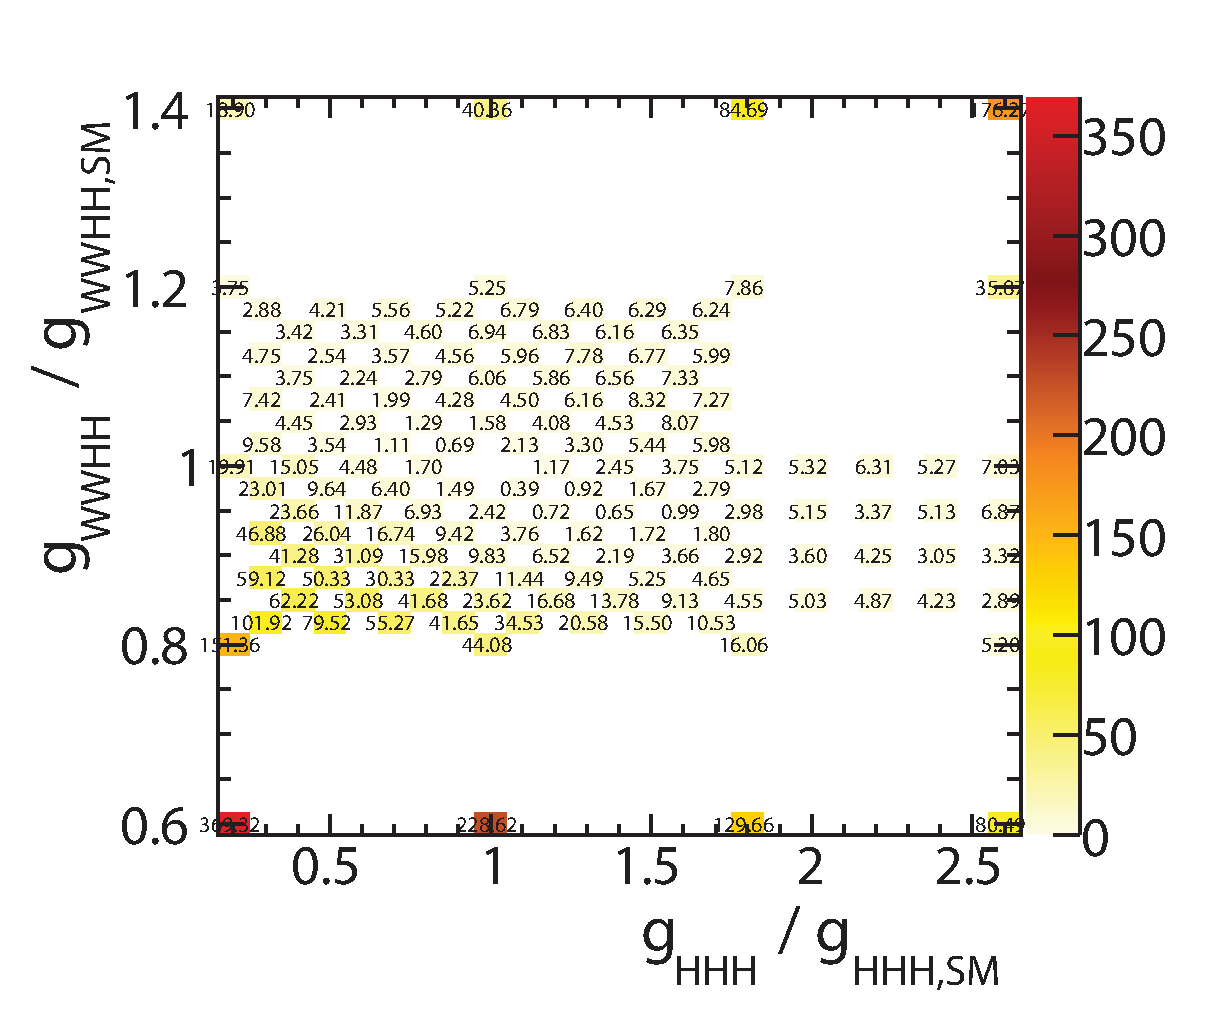
\includegraphics[width=\textwidth]{doubleHiggs/extraction/new/chi2Rosa4mhh2HT2}
    \caption{\eeToHHbbbb}
    \label{fig:doubleHiggsCouplingChi2bbbb}
  \end{subfigure}
\caption[$\chi^2$ as a function of $\gHHH/\gHHH_{SM}$ and  $\gWWHH/\gWWHH_{SM}$  at \rootS{3}]%
   {The $\chi^2$ for the \eeToHH process as a function of the $\gHHH/\gHHH_{SM}$ and  $\gWWHH/\gWWHH_{SM}$ at \rootS{3}, using sub-channel hadronic \WW decay of \eeToHHbbWW and sub-channel, assuming an integrated luminosity of  3000$fb^{-1}$.}
   \label{fig:doubleHiggsCouplingChi2Separate}
\end{figure}

Two sub-channels, hadronic \WW decay of \eeToHHbbWW and \eeToHHbbbb, are combined to increase the statistical precision on the coupling measurements.  To avoid statistical fluctuations in the sample, a toy MC experiment is performed. The SM coupling samples are treated as a data template set. 100000 data sets are generated by fluctuating the event number in each kinematic bin in the data template set according to Poisson distribution.  The $\chi^2$ is performed and summed using these generated data sets as the observed data. The summed $\chi$ is then averaged over the number of  data sets (100000) and normalised such that the $\chi^2$ at the  SM coupling is 0. Since only the difference between the non-SM and SM $\chi^2$ is used for the coupling measurements, the normalisation does not affect the measurements and helps to ease the visualisation. \FIGURE{fig:doubleHiggsCouplingChi2Ave} shows the normalised $\chi^2$ after averaging over the toy MC experiments as a function of $\gHHH/\gHHH_{SM}$ and $\gWWHH/\gWWHH_{SM}$. The $\chi^2$ changes slowly along the anti-diagonal which is similar to the cross section plot.

\begin{figure}[!tbp]
    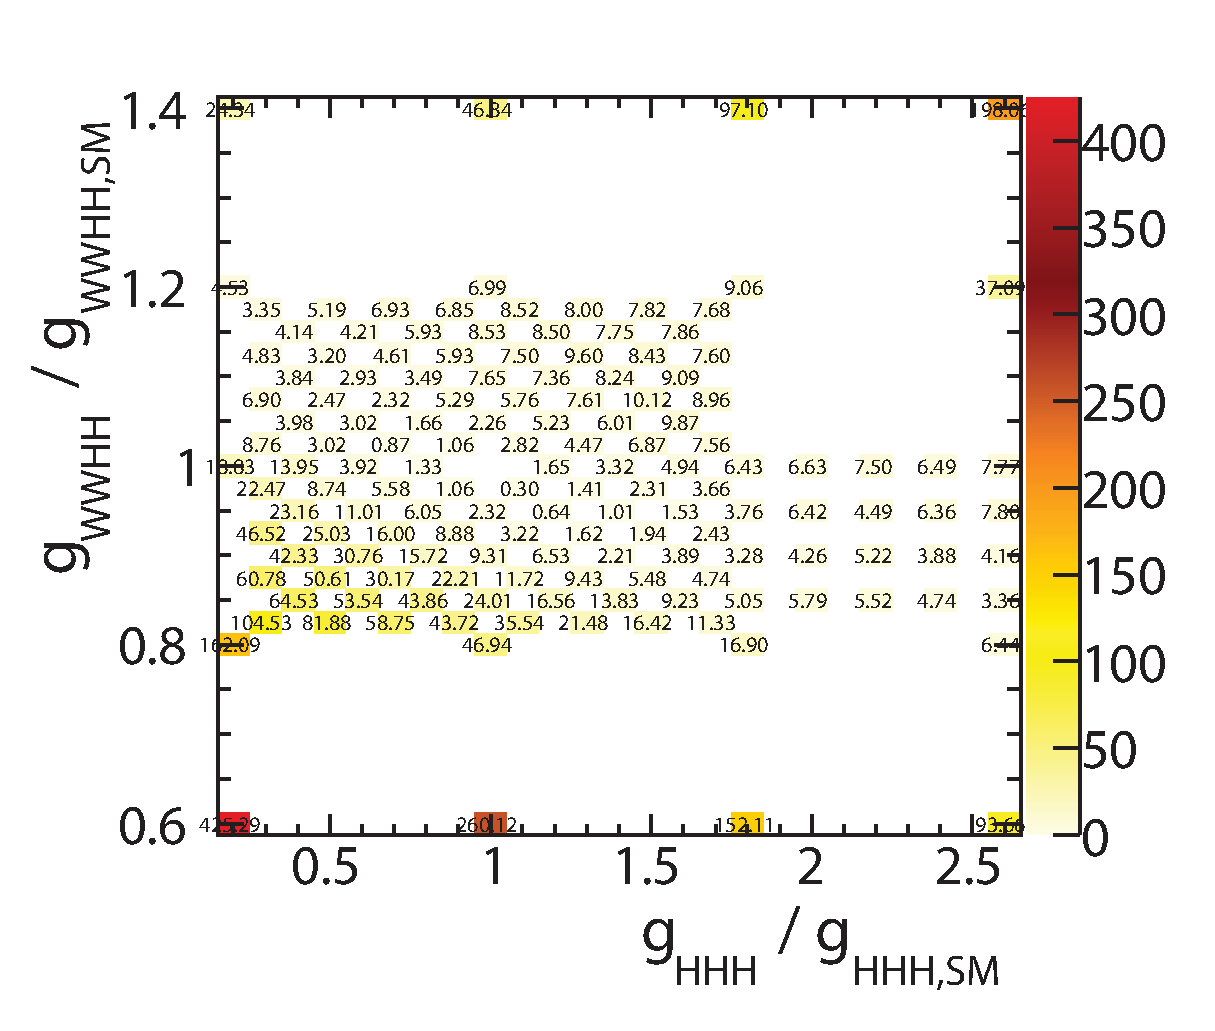
\includegraphics[width=0.85\textwidth]{{doubleHiggs/extraction/new/chi2CombineAve4mhh2HT2}}
\caption{Normalised $\chi^2$, after averaging the toy MC experiments, as a function of $\gHHH/\gHHH_{SM}$ and  $\gWWHH/\gWWHH_{SM}$, combining hadronic decay \eeToHHbbWW and \eeToHHbbbb sub-channels, assuming an integrated luminosity of  3000$fb^{-1}$.}
   \label{fig:doubleHiggsCouplingChi2Ave}
\end{figure}


\begin{figure}[!tbp]
    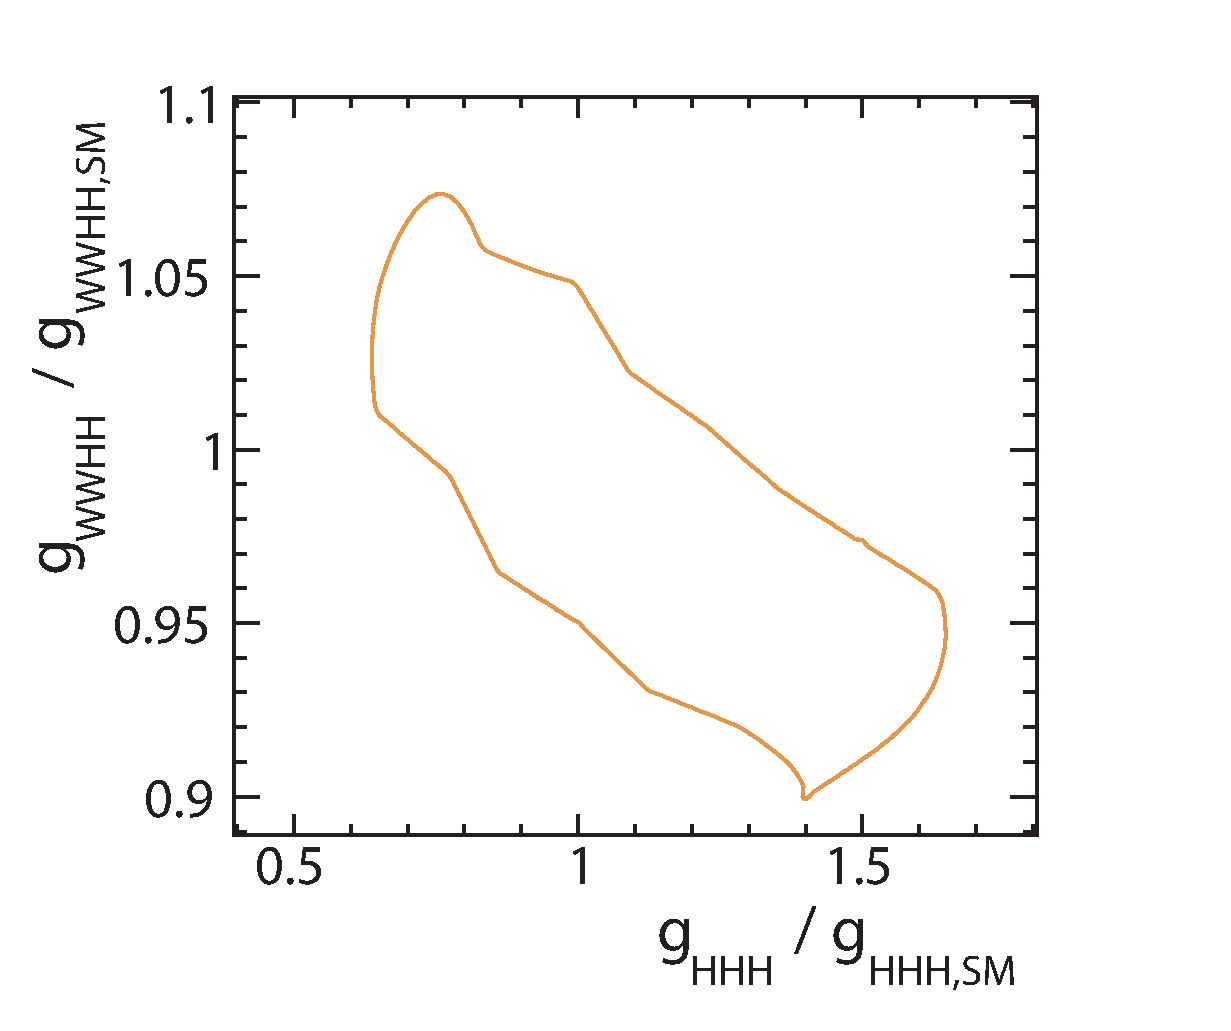
\includegraphics[width=0.85\textwidth]{doubleHiggs/extraction/new/contourCOmbineAve3}
\caption{Contour plot of 68\% confidence ($\chi^2 = 2.3$) , after averaging the toy MC experiments, as a function of $\gHHH/\gHHH_{SM}$ and  $\gWWHH/\gWWHH_{SM}$,  combining hadronic \WW  decay of \eeToHHbbWW and \eeToHHbbbb sub-channels, assuming an integrated luminosity of  3000$fb^{-1}$.}
   \label{fig:doubleHiggsCouplingChi2Countour}
\end{figure}

Since there are two couplings in this $\chi^2$ surface, the degree of freedom for this fit is 2. A contour of 68\% confidence ($\chi^2 = 2.3$) can be drawn by interpolating between points on the surface. \FIGURE{fig:doubleHiggsCouplingChi2Countour} shows the contour. The counter can be sliced one dimensionally to extract the uncertainty of one coupling for a given value of the other coupling. For example:
\begin{equation}
\frac{\Delta\gWWHH}{\gWWHH} \simeq 4.9\% \text{ for \gHHH = $\gHHH_{SM}$}
\end{equation}
\begin{equation}
\frac{\Delta\gHHH}{\gHHH} \simeq 29\% \text{ for \gWWHH = $\gWWHH_{SM}$}
\end{equation}

The statistical precisions on \gWWHH and \gHHH are much better at the \CLIC than at the current \LHC or at the high luminosity upgraded \LHC \cite{Contino:2010mh}.
